  \documentclass[english,msc,numbers]{coppe}

\usepackage{amsmath,amssymb}
\usepackage[utf8]{inputenc}
\usepackage{hyperref}
\usepackage{longtable}
\usepackage{booktabs}

\providecommand{\tightlist}{%
  \setlength{\itemsep}{0pt}\setlength{\parskip}{0pt}}

\makelosymbols
\makeloabbreviations

\begin{document}

  \title{Prediction of Petrophysical Properties Using Machine Learning and Hierarchical Multi-Task Linear Models}
  \foreigntitle{Previsão de Propriedades Petrofísicas Utilizando Modelos de Aprendizado de Máquina e Modelos Lineares Hierárquicos Multi-Task}
    \author{Marcelo}{Ramalho Albuquerque}
  

    \advisor{Prof.}{Carlos}{Eduardo Pedreira}{Ph.D}
  

    \examiner{Prof.}{Carlos Eduardo Pedreira, Ph.D}{}
    \examiner{Prof.}{Geraldo Bonorino Xexéo, D.Sc.}{}
    \examiner{Dr.}{Rodrigo Surmas, D.Sc.}{}
    \department{PESC}
  \date{09}{2020}

    \keyword{petrophysics}
    \keyword{machine learning}
    \keyword{hiearchical linear regression}
  
  \maketitle

  \frontmatter
  \dedication{I just wondered how things were put together - Claude Shannon}

    \chapter*{Agradecimentos}
  Aos meus pais, pelo cuidado e amor com que criaram todos os seus filhos.
  
  \par
  
  Ao professor Pedreira, pelo compartilhamento de conhecimento, sabedoria e orientação.
  
  \par
  
  Aos colegas de laboratório da Petrobras, pelo apoio e pelos conhecimentos compartilhados e construídos.
  
  \par
  
  À Petrobras, pela oportunidade e incentivo ao desenvolvimento dos seus funcionários e da ciência.
  
  \par
  
  À Bibi, pela paciência, carinho e amor!
 \begin{abstract}
Petrophysical characterization of reservoir rocks is a fundamental step in the evaluation of oil reservoirs, and is usually executed through laboratory experiments that incur in large costs and schedules. In this work, statistical techniques and machine learning models were evaluated fo the estimation of absolute permeability, oil-water capillary pressure and water-oil relative permeability curves, using mercury injection porosimetry, absolute permeability and porosity data. Through the exploration of several feature engineering and modeling strategies, machine learning and statistical models were assessed and compared to classical linear methods. Multi-task and hierarchical linear models were also evaluated for the estimation of special core analysis parameters from mecrcury injection porosimetry and routine core analysis data. On the evaluated dataset, hiearchical linear models were shown to have better precision, consistency and lower posterior uncertainty metrics when compared to simple linear regression models.
 \end{abstract}
  \begin{foreignabstract}
A caracterização petrofísica de rochas reservatório é uma etapa fundamental na avaliação de reservatórios de petróleo e é normalmente realizada através de ensaios laboratoriais que incorrem em custos e prazos significativos. Neste trabalho, foram avaliadas técnicas estatísticas e de aprendizado de máquina na estimativa de permeabilidade absoluta, curvas de pressão capilar óleo-água e curvas de permeabilidade relativa água-óleo, a partir de dados de porosimetria por intrusão de mercúrio, permeabilidade absoluta e porosidade. A partir da extração de diversas características das curvas de pressão capilar por intrusão de mercúrio, algoritmos de aprendizado de máquina e métodos estatísticos para a estimativa destas propriedades foram avaliados e comparados a métodos clássicos da literatura. Métodos lineares hierárquicos e multi-task foram avaliados para estimativa de curvas de pressão capilar óleo-água e permeabilidade relativa água-óleo. Foi demonstrado o efeito de regularização dos modelos lineares hierárquicos, que resultaram em modelos mais precisos, coerentes e com menor incerteza a posteriori.
  \end{foreignabstract}
  \tableofcontents
  \listoffigures

  \listoftables
  \printlosymbols
  \printloabbreviations

  \mainmatter

  \hypertarget{introduction}{%
  \chapter{Introduction}\label{introduction}}
  
  Since the beginning of the 20th century, oil and the combustion engine have transformed many aspects of modern society in fundamental ways. As a cheap and reliable energy source, oil provided the means for revolutions in transportation, manufacturing, commerce and human behavior, in general. It remains a cornerstone of our society in 2020.
  
  As knowledge of the warming effects of carbon in earth's atmosphere is further developed, conscious and economically sustainable exploitation of remaining oil reserves becomes paramount (Mackay \protect\hyperlink{ref-Mackay2009}{2009}). The high volatility of oil prices induced by supply and demand shocks in recent years further complicates the assessment of oil and gas projects.
  
  Reservoir engineering is a branch of petroleum engineering that studies fluid flow through porous hydrocarbon bearing rocks (Dake \protect\hyperlink{ref-Dake2015}{2015}). Assessment of oil and gas exploitation projects is commonly performed using numerical simulation models that incorporate geological, fluid and petrophysical information to predict oil and gas production curves. Reservoir uncertainties are particularly important at the beginning of a project, when few wells have been drilled, fluid and rock samples are scarce, and no production data is available.
  \begin{figure}
  
  {\centering 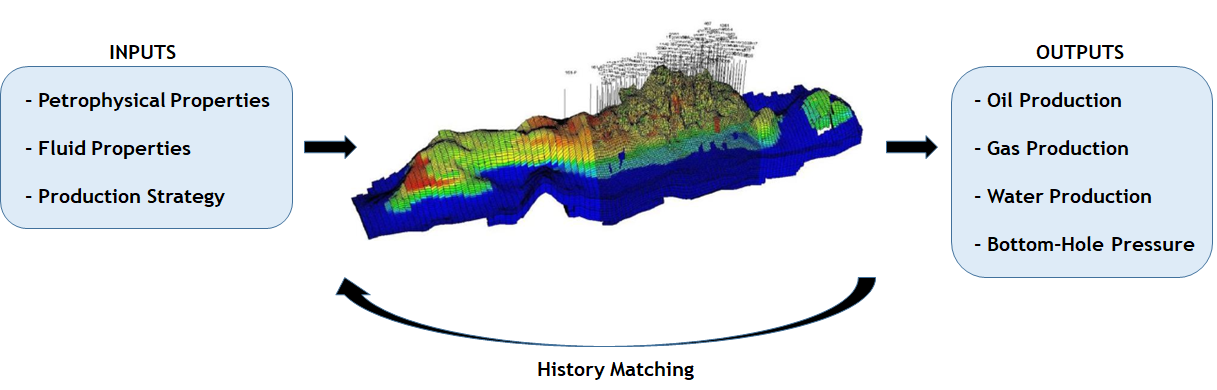
\includegraphics[width=1\linewidth]{figure/1-1-ResEng} 
  
  }
  
  \caption{Reservoir Engineering Simulation Models}\label{fig:res-eng}
  \end{figure}
  Petrophysical characterization entails the evaluation of physical and chemical properties of porous media, and its interaction with reservoir fluids. It is commonly performed through laboratory experiments, known in the petroleum industry as routine and special core analysis (Peters \protect\hyperlink{ref-Peters2012}{2012}). Routine petrophysical experiments characterize rock porosity and absolute permeability, are considered inexpensive and can be performed in little time, usually taking no more than a couple of days per sample. Special core analysis, characterize properties related to the balance of viscous and capillary forces acting at reservoir conditions and, in many situations, can be expensive and demand long experiments, which can take up to several months to be executed (Tiab and Donaldson \protect\hyperlink{ref-Tiab2004}{2004}).
  
  In this work, statistical methods were evaluated for the estimation of petrophysical properties using as input Mercury Injection Capillary Pressure (MICP) and routine core analysis data. This work is organized as follows: on chapter \ref{petrophysical-properties}, petrophysical measurement methods and properties are briefly described; on chapter \ref{kabs-regression}, black-box machine learning models for the prediction of absolute permeability from MICP data are evaluated and compared to classical linear models; on chapter \ref{hierarchical-linear-regression}, linear models for the prediction of special core analysis properties, using multi-task and hierarchical models, are studied; limitations and desirable features of the evaluated methods are further discussed on chapter \ref{conclusion}.
  
  \hypertarget{petrophysical-properties}{%
  \chapter{Measuring Petrophysical Properties}\label{petrophysical-properties}}
  
  The measurement of petrophysical properties is performed through specialized laboratory experiments, which in the petroleum industry are classified as routine or special core analysis (SCAL), depending on the experiment complexity and on its investigated properties.
  
  The analyzed rock samples may be extracted from well cores or from open borehole sidewall sampling tools, and can measure from one to several centimeters (Kennedy \protect\hyperlink{ref-Kennedy2015}{2015}). The rock samples are commonly extracted as cylindrical plugs, but can also have irregular shapes, case in which they are referred to as rock fragments.
  
  \hypertarget{routine-core-analysis}{%
  \section{Routine Core Analysis}\label{routine-core-analysis}}
  
  Experimental measurements of a rock sample pore volume \(V_p\), grain volume \(V_g\), porosity \(\phi\) and absolute permeability \(k_{abs}\) are commonly referred to as routine core analysis.
  
  Porous media can be pictorially described as being constituted of grain and pore spaces (Figure \ref{fig:porous-media}). The percentage of the total space occupied by pores is known as rock porosity. \(V_p\) and \(\phi\) measurements are important for the evaluation of hydrocarbon reserve volumes.
  \begin{figure}
  
  {\centering 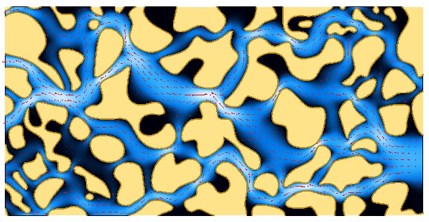
\includegraphics[width=1\linewidth]{figure/2-1-Porous-media} 
  
  }
  
  \caption{Pore media grain and pore spaces}\label{fig:porous-media}
  \end{figure}
  \begin{equation} 
    \phi = \frac{V_p}{V_p + V_g}
    \label{eq:phi}
  \end{equation}
  At reservoir conditions, porous space is filled by either water, oil or gas, each of which in a separate phase. The percentage of the porous volume occupied by water, oil or gas is known as water, oil or gas saturation, respectively.
  \begin{equation} 
    S_f = \frac{V_f}{V_p},\quad \text{for} \;f \; \text{in} \; {w, o, g}
    \label{eq:saturation}
  \end{equation}
  Darcy's law \eqref{eq:darcy} describes the linear relationship between instantaneous flow rate \(q\) and a pressure gradient \(\frac{\partial p}{\partial x}\) in laminar single-phase flow (Tiab and Donaldson \protect\hyperlink{ref-Tiab2004}{2004}). Given a stable steady-state single-phase flow, the porous media absolute permeability \(k_{abs}\) is directly proportional to the instantaneous flow rate \(q\), fluid viscosity \(\mu\), and is inversely proportional to the pressure gradient \(\frac{\partial p}{\partial x}\) and cross-sectional area \(A\).
  \begin{equation} 
    q = k_{abs}\frac{A}{\mu}\frac{\partial p}{\partial x}
    \label{eq:darcy}
  \end{equation}
  \hypertarget{special-core-analysis}{%
  \section{Special Core Analysis}\label{special-core-analysis}}
  
  Measurement of multiphase properties of porous media, on which both viscous and capillary forces may be relevant, is usually more complex and incurs in longer and costlier experiments when compared to single-phase routine core analysis measurements.
  
  \hypertarget{mercury-injection-capillary-pressure}{%
  \subsection{Mercury Injection Capillary Pressure}\label{mercury-injection-capillary-pressure}}
  
  In multi-phase porous systems, due to different interaction characteristics between fluid and solid phases, the attraction between the molecules of one of the fluid phases and the solid surfaces may be greater than that of the other fluid phase. This physical behavior is known as wettability, and it is responsible for capillary forces and related phenomena.
  
  For a given multiphase porous system, with a surface tension \(\sigma\) between fluid phases, wettability may be quantified by the contact angle \(\theta\) formed by the fluid phase boundary-solid interface, as depicted in Figure \ref{fig:contact-angle}.
  
  The Young-Laplace equation describes the capillary pressure sustained across the interface between fluids at a pore throat constriction (Tiab and Donaldson \protect\hyperlink{ref-Tiab2004}{2004}). A heterogeneous porous system is connected by pore throats of several different radii. For a system consisting of mercury and mercury vapor, with surface tension \(\sigma_{Hg-air}\) and contact angle \(\theta_{Hg-air}\) with the rock surface, the relationship between capillary pressure and pore throat radius r may be described by equation \eqref{eq:young}. Capillary forces may strongly affect the distribution of fluid phases in the porous space.
  \begin{figure}
  
  {\centering 
\includegraphics[width=0.8\linewidth]{figure/2-2-Contact-Angle} 
  
  }
  
  \caption{Contact Angle between fluid phase boundary and solid surface}\label{fig:contact-angle}
  \end{figure}
  \begin{equation} 
    P_c = \frac{2\sigma_{Hg-air} \cos{\theta_{Hg-air}}}{r}
    \label{eq:young}
  \end{equation}
  A Mercury Injection Capillary Pressure (MICP) experiment consists of pre-specified and controlled mercury injection steps in a porous medium, previously subjected to a vacuum. It is usually performed on rock fragments with around one cubic centimeter, which allows it to be executed both in well core and sidewall sample fragments. Automated acquisition systems for MICP are commercially available (Micromeritics \protect\hyperlink{ref-Micromeritics2020}{2020})(Figure \ref{fig:autopore}), making it a relatively fast and cheap experiment.
  
  A fixed pressure stabilization time and a geometric progression sequence of increasing pressure steps is defined before each MICP experiment. At each pressure step, after the pre-defined pressure stabilization time, the volume of intruded mercury in the rock sample pore space is recorded. Given calibrated mercury-mercury-vapor surface tension \(\sigma_{hg-air}\) and contact angle \(\theta_{hg-air}\), each pressure step may be associated with a pore throat radius according to equation \eqref{eq:young}. The cumulative intruded mercury volume \(V_{hg}\) at each step, thus, corresponds to the porous volume accessible by pore throats with radius equal to or smaller than the relationship given by equation \eqref{eq:young}. Mercury saturation \(S_{hg}\) at each step may be calculated using equation \eqref{eq:shg}.
  \begin{figure}
  
  {\centering 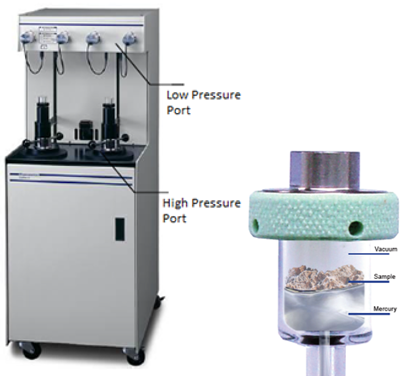
\includegraphics[width=0.5\linewidth]{figure/2-3-Autopore} 
  
  }
  
  \caption{AutoPore IV Series Mercury Porosimeter (left) and glass penetrometer (right) used in automated MICP acquisitions.}\label{fig:autopore}
  \end{figure}
  \begin{equation} 
    S_{hg} = \frac{V_{hg}}{V_T}
    \label{eq:shg}
  \end{equation}
  The total fragment volume \(V_T\) is estimated during the experimental data interpretation procedure, using the difference of the total glass bulb volume and the intruded mercury volume necessary to ``envelope'' the rock fragment and start intruding the porous space. This happens at a pressure known as entrance capillary pressure \(P_e\) The determination of the exact value of this entrance capillary pressure may introduce uncertainty on experimental results, particularly for very irregular shaped or vuggy rock samples.
  
  The recorded capillary pressure \(P_c\) and mercury saturation \(S_{hg}\) values form a capillary pressure curve, whose format is directly related to the distribution of accessible pore volume in the porous medium of the rock sample. Figure \ref{fig:pc-curves} shows several capillary pressure curves acquired in MICP experiments.
  
  A widely used transformation of capillary pressure curves is described by equation \eqref{eq:pdf} (Lenormand \protect\hyperlink{ref-Lenormand2003}{2003}), which constructs a probability distribution of accessible pore volume as a function of the logarithm of the associated pore throat radius \(r\). Figure \ref{fig:pdf-curves} shows pore volume probability distribution curves \(p(\log{r})\), for the same MICP experiments depicted in Figure \ref{fig:pc-curves}.
  \begin{equation} 
    p(\log{r}) = \frac{dS_{hg}}{d \log{P_c}}
    \label{eq:pdf}
  \end{equation}
  \begin{figure}
  
  {\centering 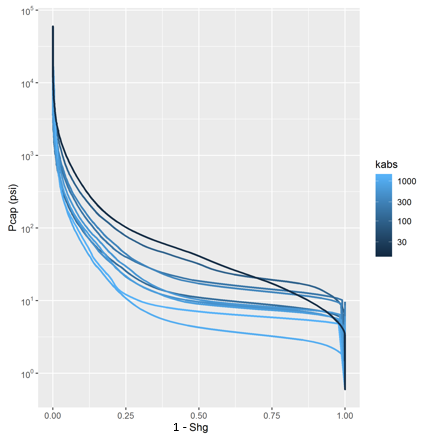
\includegraphics[width=0.9\linewidth]{figure/2-4-Pc-curves} 
  
  }
  
  \caption{Mercury Injection Capillary Pressure Curves for several rock samples, colored by absolute permeability.}\label{fig:pc-curves}
  \end{figure}
  \begin{figure}
  
  {\centering 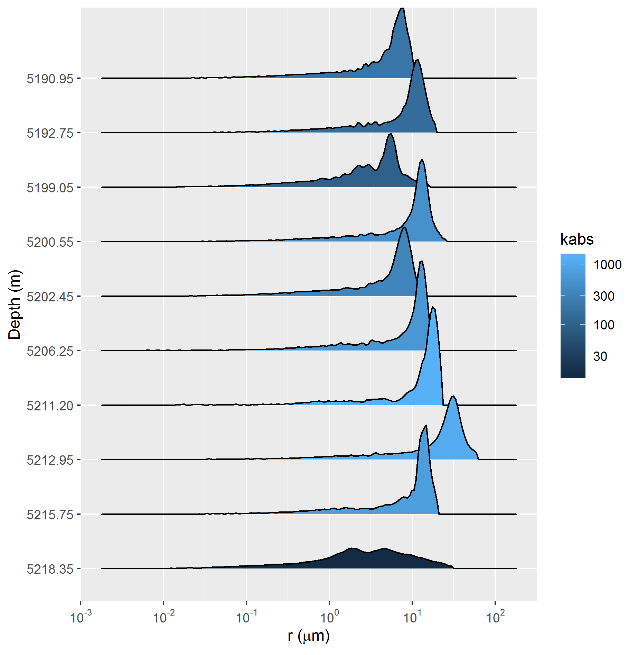
\includegraphics[width=0.9\linewidth]{figure/2-5-pdf-curves} 
  
  }
  
  \caption{Accessible pore volume probability distribution curves p(log r), for the same MICP experiments depicted in Figure 2.4.}\label{fig:pdf-curves}
  \end{figure}
  Several authors have proposed correlations between capillary pressure curve features and absolute permeability (Kolodzie \protect\hyperlink{ref-Kolodzie1980}{1980}; Pittman \protect\hyperlink{ref-Pittman1992}{1992}; Purcell \protect\hyperlink{ref-Purcell1949}{1949}; Swanson \protect\hyperlink{ref-Swanson1981}{1981}), among others. These correlations will be further explorer on chapter \ref{kabs-regression}.
  
  In this work, a dataset of 2324 MICP curves acquired on rock fragments of sandstone and carbonate reservoirs from several Brazilian reservoirs was compiled. Routine and special core analysis results, performed on core sample plugs and sidewall samples extracted from the same well depths as the rock fragments were incorporated in the dataset.
  
  Given that the size of the rock fragments utilized for MICP measurements were in many cases many times smaller than the size of the corresponding core sample plugs and sidewall samples, where routine and special core analysis were performed, it is very likely that, for many samples, the rock fragments may not constitute a representative volume of the porous space (Blunt \protect\hyperlink{ref-Blunt2017}{2017}). Indeed, as illustrated in Figure \ref{fig:heterogeneity}, it is possible to assess that heterogeneous reservoirs display many more outlier samples on correlations between MICP and core analysis data, when compared to more homogeneous reservoirs.
  \begin{figure}
  
  {\centering 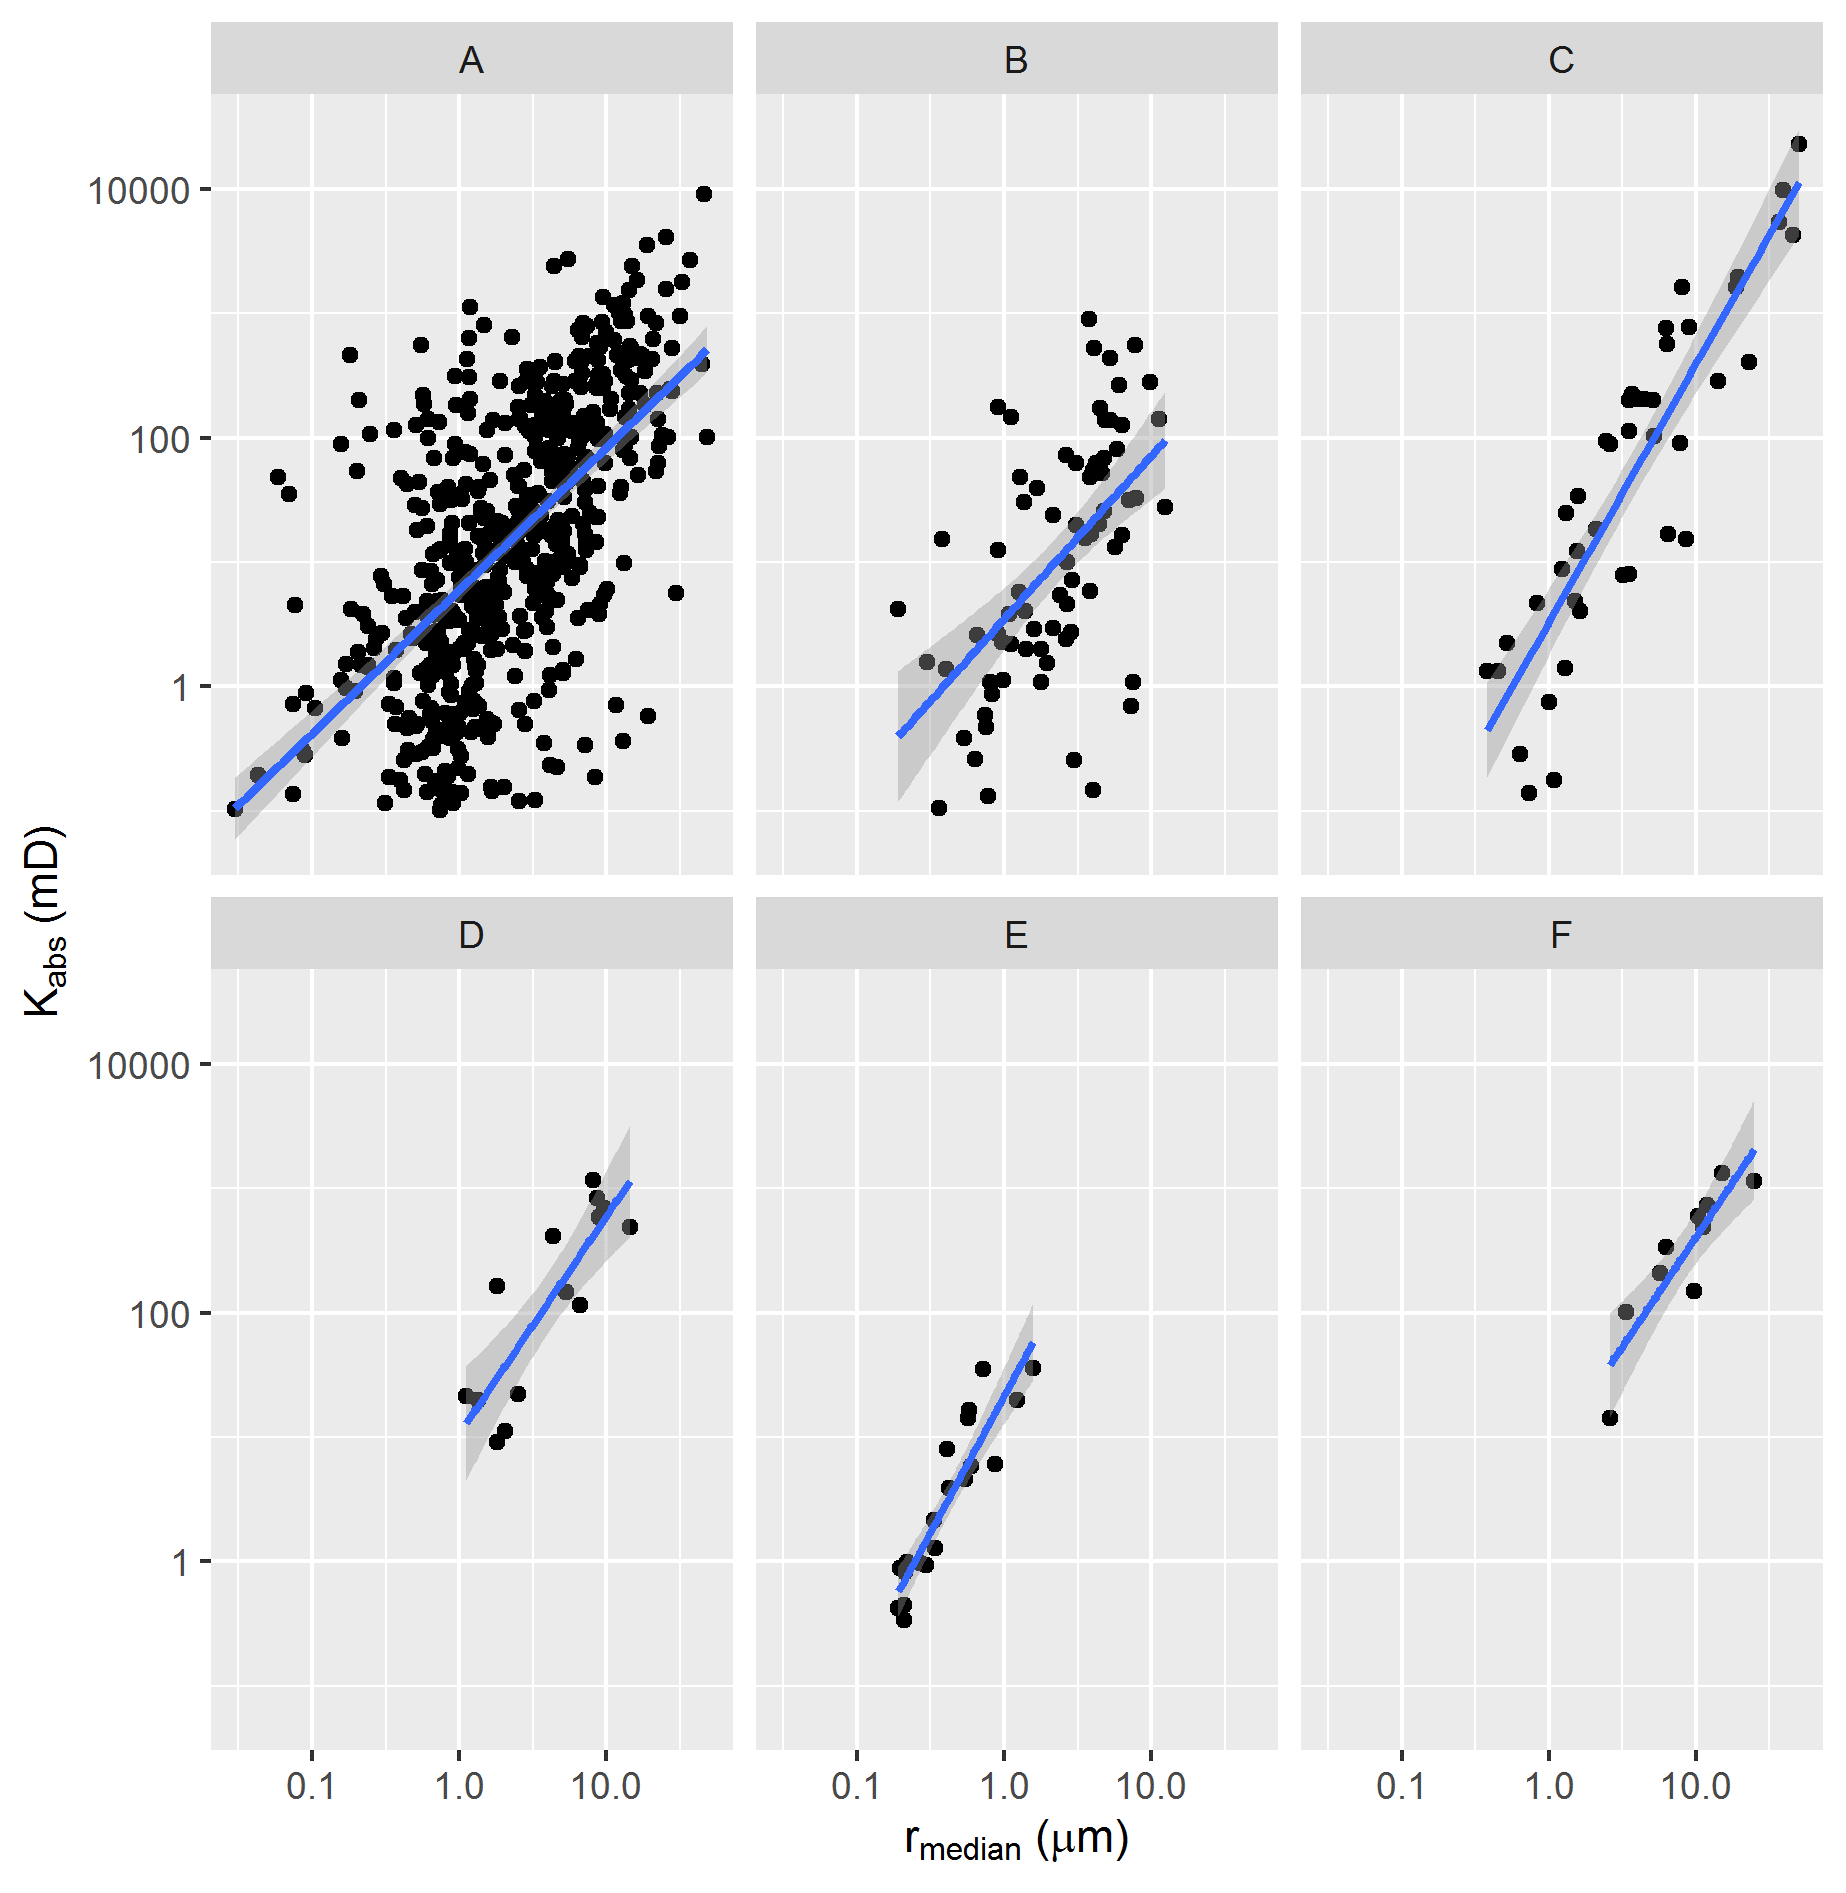
\includegraphics[width=0.85\linewidth]{figure/2-6-heterogeneity} 
  
  }
  
  \caption{Relationship between median pore throat radius and absolute permeability of several different reservoirs, from most to least heterogeneous}\label{fig:heterogeneity}
  \end{figure}
  \hypertarget{centrifuge-capillary-pressure}{%
  \subsection{Centrifuge Capillary Pressure}\label{centrifuge-capillary-pressure}}
  
  The centrifuge method is a standard technique for capillary pressure curve estimation of porous media. The method consists of imposing a capillary pressure profile on a rotating rock sample through centrifugal acceleration imposition in increasing rotation speed steps, and recording the average sample saturation at each step (Tiab and Donaldson \protect\hyperlink{ref-Tiab2004}{2004}). The fundamental equations that describe the method were developed by Hassler and Brunner (Hassler and Brunner \protect\hyperlink{ref-Hassler1945}{1945}):
  \begin{figure}
  
  {\centering 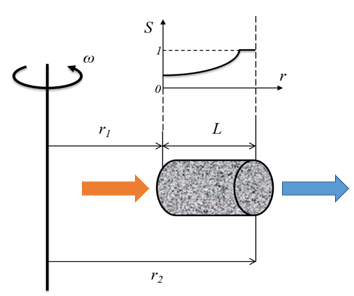
\includegraphics[width=0.6\linewidth]{figure/2-7-centrifuge-geometry} 
  
  }
  
  \caption{Drainage Oil-Water Centrifuge capillary pressure experiment geometry.}\label{fig:centrifuge-geometry}
  \end{figure}
  \begin{equation} 
    P_c = \frac{1}{2}\omega^2\Delta \rho (r^2-r_{2}^{2})
    \label{eq:pc}
  \end{equation}
  \begin{equation} 
    B = 1 - (\frac{r_1}{r_2})^2
    \label{eq:B}
  \end{equation}
  \begin{equation} 
    S_w = \frac{V_w}{V_p} = \frac{V_w}{V_w + V_o}
    \label{eq:Sw}
  \end{equation}
  \begin{equation} 
    \overline{S_w}(P_c)=\frac{(1+\sqrt{1-B})}{2}\int_0^1{\frac{S_w(xP_c)}{\sqrt{1-Bx}}} dx
    \label{eq:meansw}
  \end{equation}
  where \(\omega\) is the centrifuge rotation speed, \(\Delta \rho\) is the difference in density between the displacing and displaced fluids, \(L\) is the rock sample length, \(r\) is the radius to the centrifuge rotation center, \(r_1\) and \(r_2\) are the radial distances to the sample extremities, \(V_p\), \(V_w\) and \(V_o\) are the sample pore, water and oil volumes, \(S_w (P_c)\) is the water saturation at a given point in the sample subjected to a \(P_c\) capillary pressure, and \(\overline{S_w}\) is the sample average water saturation.
  
  Several methods have been proposed for the estimation of capillary pressure curves from centrifuge experiments. These methods may be classified as direct or inverse according to how they solve the centrifuge saturation equation. Direct methods use several proposed differential and integral approximations of the saturation equation to directly estimate capillary-pressure curves from centrifuge experiment measurements at discrete capillary-pressure steps (Forbes \protect\hyperlink{ref-Forbes1994}{1994}; Hassler and Brunner \protect\hyperlink{ref-Hassler1945}{1945}; Skuse, Flroozabadl, and Ramey Jr. \protect\hyperlink{ref-Skuse1992}{1992}). Inverse methods parameterize capillary-pressure curves and solve the saturation equation using non-linear regression (Bentsen \protect\hyperlink{ref-Bentsen1977}{1977}) or linear regression with spline basis functions (Nordtvedt and Kolltvelt \protect\hyperlink{ref-Nordtvedt1991}{1991}).
  \begin{figure}
  
  {\centering 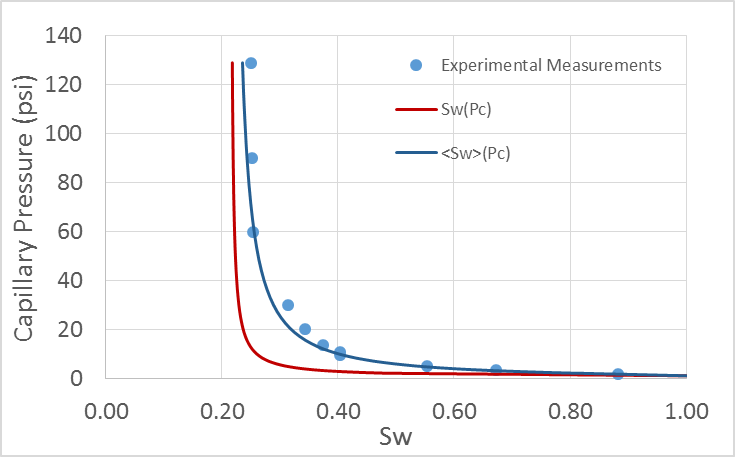
\includegraphics[width=0.7\linewidth]{figure/2-8-centrifuge-experiment} 
  
  }
  
  \caption{Estimation of capillary pressure curve from centrifuge measurements.}\label{fig:centrifuge-experiment}
  \end{figure}
  In this work, a dataset of 135 capillary pressure curves estimated from centrifuge experiments was compiled. Using the parameterization \eqref{eq:albu}, proposed in (Albuquerque et al. \protect\hyperlink{ref-Albuquerque2018}{2018}), each of the capillary pressure curves was fitted using a least-squares minimization procedure, with parameters \(S_{wi}\), \(P_e\), \(\alpha\) and \(\beta\).
  \begin{equation} 
    S_w(P_c, S_{wi}, \alpha, \beta, P_w) = \frac{1+\alpha S_{wi}(P_c - P_e)^\beta}{(1+\alpha (P_c - P_e)^\beta}
    \label{eq:albu}
  \end{equation}
  \begin{figure}
  
  {\centering 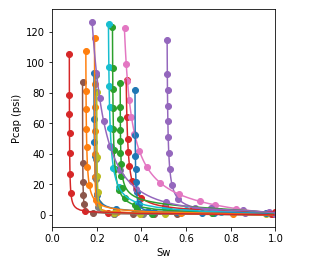
\includegraphics[width=0.7\linewidth]{figure/2-9-pcc-dataset} 
  
  }
  
  \caption{Sample of the experimental capillary pressure curve dataset (points) and fitted capillary pressure model (lines).}\label{fig:pcc-dataset}
  \end{figure}
  This parameterization is such that for high values of capillary pressure, water saturation \(S_w\) approaches \(S_{wi}\), a parameter thus named irreducible water saturation. In a drainage capillary pressure model, the smallest pressure at which the saturation of the sample can be reduced from one hundred per cent is termed ``entrance'' capillary pressure (Peters \protect\hyperlink{ref-Peters2012}{2012}), modeled by parameter \(P_e\) in equation \eqref{eq:albu}. The remainder parameters \(\alpha\) and \(\beta\) are associated with the capillary pressure curve steepness and shape.
  \begin{equation} 
    \lim_{P_c \to +\infty} S_w = S_{wi}
    \label{eq:lim-swi}
  \end{equation}
  \begin{equation} 
    P_c(S_{w}=1) = P_e
    \label{eq:lim-pe}
  \end{equation}
  Considering a transformation analogous to the one utilized for mercury injection capillary pressure curves \eqref{eq:pdf}, pore volume probability distribution curves \(p(\log r)\) may be estimated from the fitted centrifuge capillary pressure curve parameters, as described by equation \eqref{eq:pdf-pcc}.
  \begin{equation} 
    p(\log r) = \frac{dS_w}{d \log{P_c}} = \frac{\alpha \beta S_{wi} (S_w - S_{wi})(P_c - P_e)^{\beta - 1}}{1 + \alpha (P_c - P_e)^\beta}
    \label{eq:pdf-pcc}
  \end{equation}
  \begin{figure}
  
  {\centering 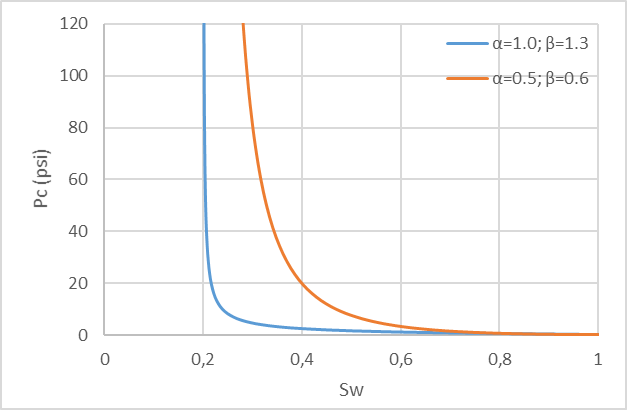
\includegraphics[width=0.7\linewidth]{figure/2-10a-pcc-params-curves} 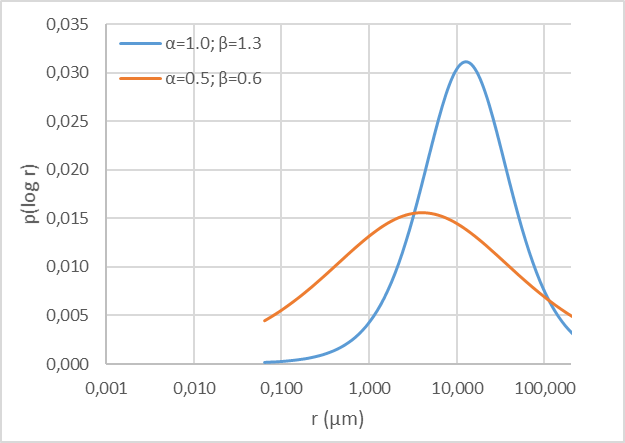
\includegraphics[width=0.7\linewidth]{figure/2-10b-pcc-params-pdf} 
  
  }
  
  \caption{Sample centrifuge capillary pressure curves, parameterized by equation (2.11), and corresponding pore volume probability distribution curves p(log r).}\label{fig:pcc-params}
  \end{figure}
  As graphically displayed in Figure \ref{fig:pcc-params}, the parameter \(\alpha\) can be shown to be associated with the location of the distribution \(p(\log{r})\) and the parameter \(\beta\) can be shown to be associated with its scale or dispersion.
  
  A dataset combining the fitted centrifuge capillary pressure curve parameters and several MICP features, detailed on chapter \ref{kabs-regression}, of rock fragments extracted from corresponding core locations was assembled. As exemplified in Figure \ref{fig:pcc-pchg}, associated pore volume distributions of corresponding centrifuge capillary pressure and MICP curves often display similar distributions, though to varying degrees as MICP curves may have been measured in rock fragments which may or may not be representative of its associated core sample pore volume. MICP experiments also cover a larger range of pore throat radius sizes and display significantly more detail, as a much tighter pressure and corresponding pore throat radius experimental grid is sampled.
  \begin{figure}
  
  {\centering 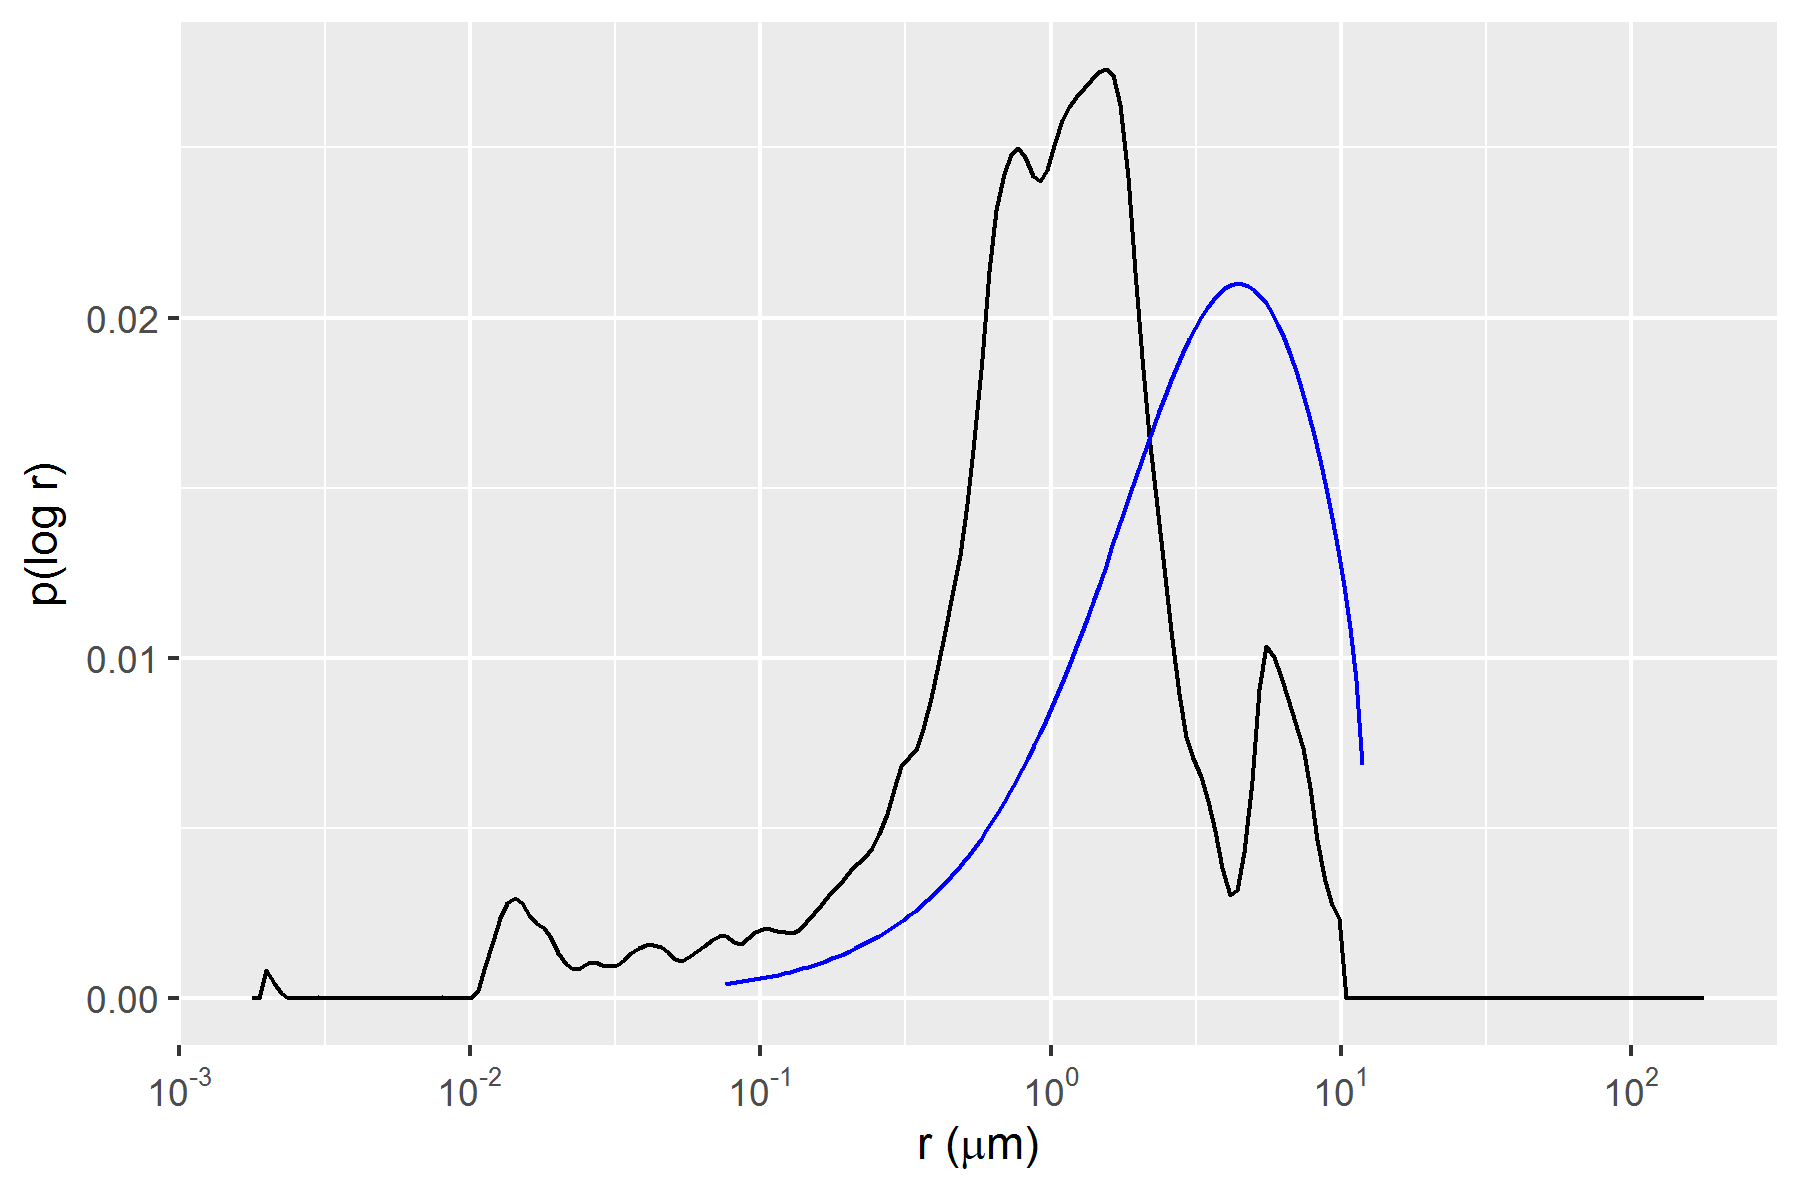
\includegraphics[width=0.9\linewidth]{figure/2-11-pcc-pchg-pdf} 
  
  }
  
  \caption{Associated pore volume distributions p(log r) of correspondent Centrifuge Capillary Pressure (blue curve) and MICP (black curve) samples.}\label{fig:pcc-pchg}
  \end{figure}
  In Figure \ref{fig:pchg-correlations}, it is possible to identify significant correlations between corresponding centrifuge capillary pressure curves \(\alpha\), \(S_{wi}\) and MICP median pore throat radius \(r_{median}\) parameters. Both \(\alpha\) and \(S_{wi}\) parameters can be seen, thus, as correlated with the location of the distribution \(p(\log{r})\).
  \begin{figure}
  
  {\centering 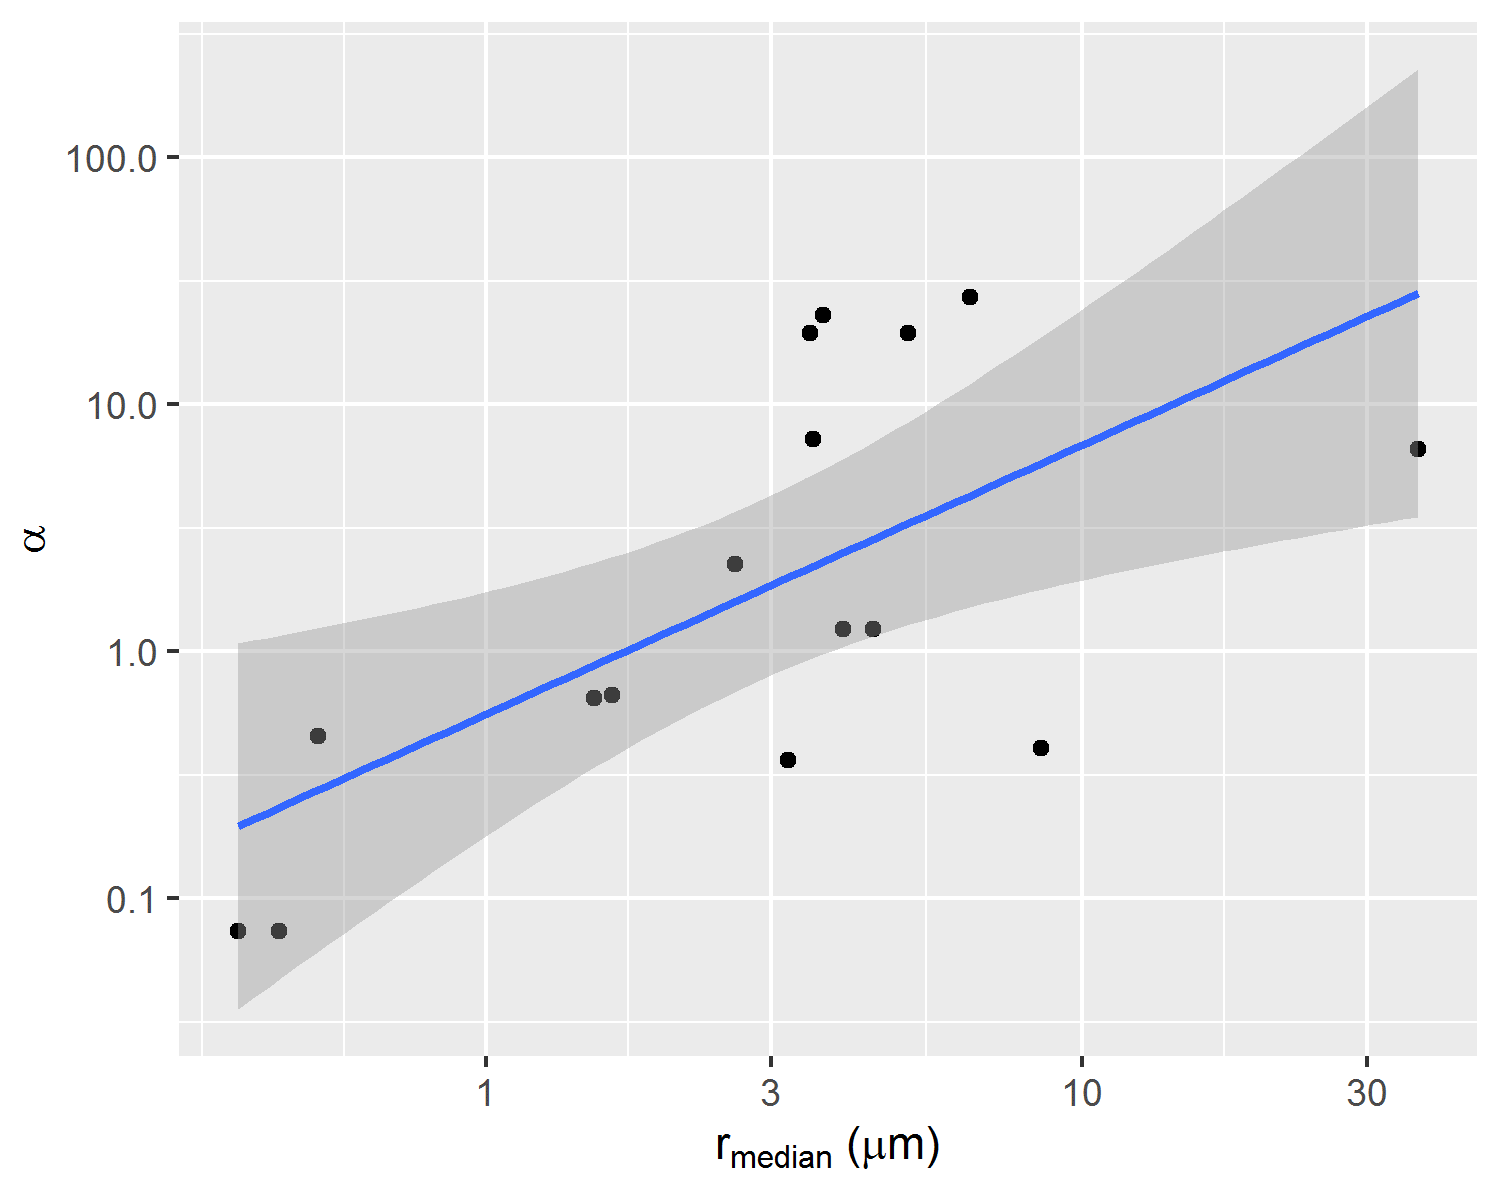
\includegraphics[width=0.45\linewidth]{figure/2-12a-correlations-pchg} 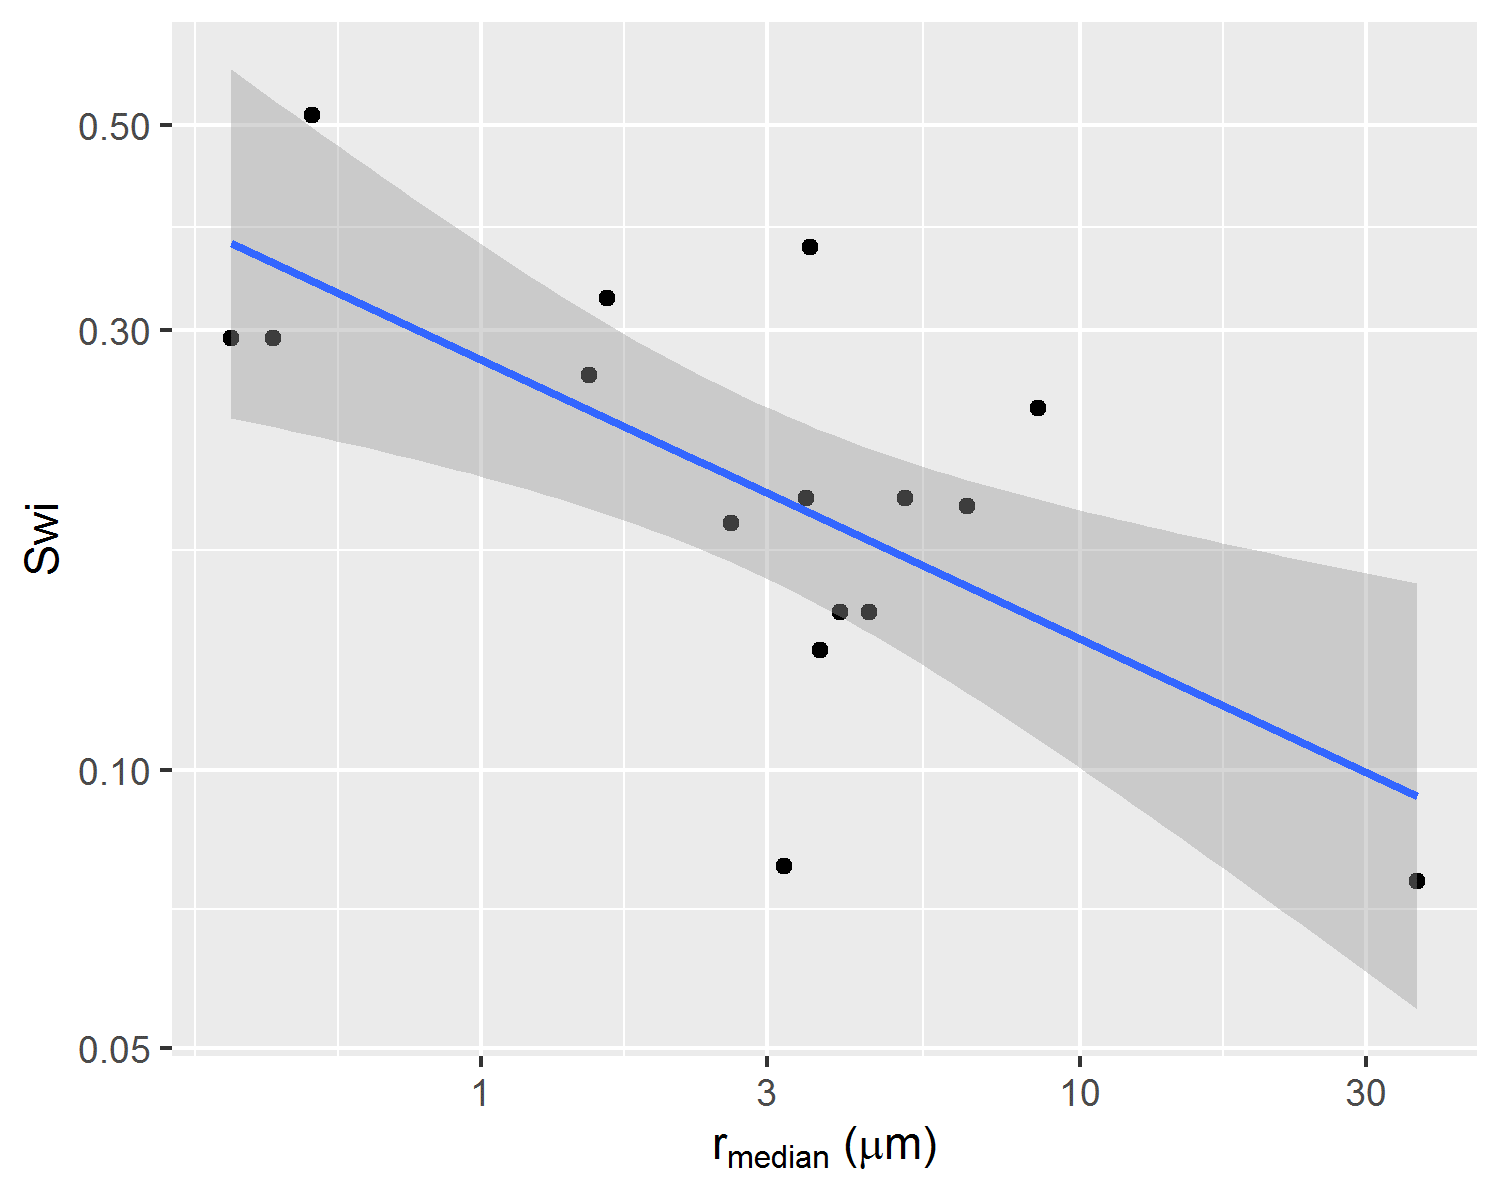
\includegraphics[width=0.45\linewidth]{figure/2-12b-correlations-pchg} 
  
  }
  
  \caption{Correlations between parameters alpha, Swi and median pore throat radius of correspondent rock fragment p(log r) distribution.}\label{fig:pchg-correlations}
  \end{figure}
  \hypertarget{relative-permeability}{%
  \subsection{Relative Permeability}\label{relative-permeability}}
  
  In porous media multiphase flow, relative permeability describes the linear proportion by which each fluid flow is penalized when compared to Darcy's law \eqref{eq:darcy}. For a water-oil two-phase flow, the following relations describe oil (\(k_{ro}\)) and water (\(k_{rw}\)) relative permeability, and the their associated fractionary water flow (\(f_{w}\)).
  \begin{equation} 
    q_o(S_w) = k_{ro}(S_w) \frac{k_{abs}A}{\mu_o L} \Delta p
    \label{eq:kro}
  \end{equation}
  \begin{equation} 
    q_w(S_w) = k_{rw}(S_w) \frac{k_{abs}A}{\mu_w L} \Delta p
    \label{eq:krw}
  \end{equation}
  \begin{equation} 
    f_w = \frac{\frac{k_{rw}}{\mu_w}}{\frac{k_{rw}}{\mu_w} + \frac{k_{ro}}{\mu_o}}
    \label{eq:fw}
  \end{equation}
  The most widely used experimental setup for water-oil relative permeability determination is the unsteady-state water-oil relative permeability experiment. In a unsteady-state water-oil relative permeability experiment, a sample initially satured at irreducible water saturation \(S_{wi}\) condition is subjected to a constant rate water injection, simulating reservoir secondary recovery water injection.
  
  During the experiment, water injection flow rate \(q_{w_{inj}}\) and exit pressure \(P_{out}\) are kept constant, and cumulative oil production \(N_p\) and pressure differential \(\Delta p\) are recorded.
  \begin{figure}
  
  {\centering 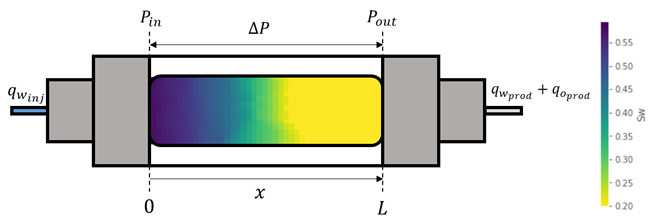
\includegraphics[width=1\linewidth]{figure/2-13-krel-experiment} 
  
  }
  
  \caption{Unsteady-state relative permeability experimental setup.}\label{fig:krel-experiment}
  \end{figure}
  \begin{equation} 
    q_{w_{inj}} = cte 
    \label{eq:qwinj}
  \end{equation}
  \begin{equation} 
    P_{out} = cte 
    \label{eq:pout}
  \end{equation}
  Unsteady state water-oil relative permeability experiments are usually interpreted using either the JBN method (Johnson, Bossler, and Naumann \protect\hyperlink{ref-Johnson1959}{1959}) or using history matched numerical simulated solutions (Lenormand and Lenormand \protect\hyperlink{ref-Lenormand2016}{2016}). Figure \ref{fig:krel-Np-dP} displays an example of recorded and history matched cumulative oil production \(N_p\) and pressure differential \(\Delta p\), obtained using maximum likelihood estimation of the relative permeability parameters that best fit the recorded experimental data.
  \begin{figure}
  
  {\centering 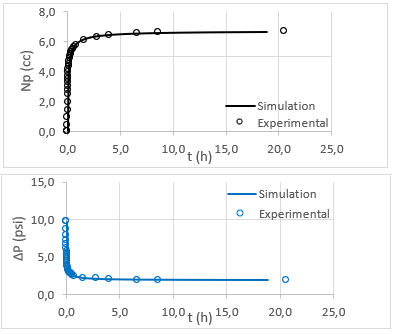
\includegraphics[width=0.7\linewidth]{figure/2-14-krel-Np-dP} 
  
  }
  
  \caption{Example of history matched experimental data.}\label{fig:krel-Np-dP}
  \end{figure}
  \begin{figure}
  
  {\centering 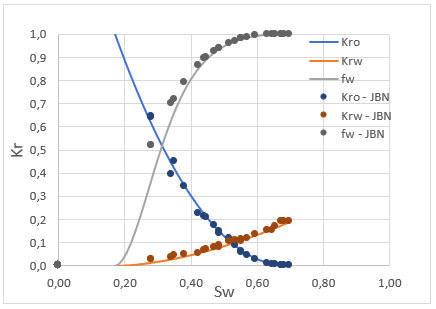
\includegraphics[width=0.7\linewidth]{figure/2-15-krel-JBN} 
  
  }
  
  \caption{Example of history matched relative permeability and fractionary flow curves compared to analytic JBN interpreted experimental results.}\label{fig:krel-JBN}
  \end{figure}
  History matching is usually performed using parametric relative permeability models and finite difference partial differential equations simulation. The Corey model (Corey \protect\hyperlink{ref-Corey1954}{1954}), given by equations \eqref{eq:swd}\eqref{eq:kro-corey}\eqref{eq:krw-corey}, is a widely used power-law model for relative permeability curves, whose parameters \(n_o\) and \(n_w\) are commonly referred to as Corey exponents.
  \begin{equation} 
    S_{wD} = \frac{S_w - S_{wi}}{1 - S_{wi} - S_{or}} 
    \label{eq:swd}
  \end{equation}
  \begin{equation} 
    k_{ro}(S_w) = k_{ro@S_{wi}}(1-S_{wD})^{n_o}
    \label{eq:kro-corey}
  \end{equation}
  \begin{equation} 
    k_{rw}(S_w) = k_{rw@S_{or}}(S_{wD})^{n_w}
    \label{eq:krw-corey}
  \end{equation}
  The LET model (Lomeland, Ebeltoft, and Thomas \protect\hyperlink{ref-Lomeland2005}{2005}), given by equations \eqref{eq:kro-let}\eqref{eq:krw-let}, was developed with six shape parameters \(L_o\), \(E_o\), \(T_o\), \(L_w\), \(E_w\), \(T_w\), and can accommodate much more flexible relative permeability curves. It is commonly used in reservoir simulation models, especially for history matching procedures that demand flexible representations of relative permeability models.
  \begin{equation} 
    k_{ro}(S_w) = k_{ro@S_{wi}}\frac{(1-S_{wD})^{L_o}}{(1-S_{wD})^{L_o} + E_o(S_{wD})^{T_o}}
    \label{eq:kro-let}
  \end{equation}
  \begin{equation} 
    k_{rw}(S_w) = k_{rw@S_{or}}\frac{(S_{wD})^{L_w}}{(S_{wD})^{L_w} + E_w(1-S_{wD})^{T_w}}
    \label{eq:krw-let}
  \end{equation}
  In this work, a dataset of 226 unsteady-state water-oil relative permeability curves was assembled. LET parameters for each of the 226 curves were fit using maximum likelihood estimation (DeGroot and Schervish \protect\hyperlink{ref-DeGroot2012}{2012}). Multivariate and multi-task linear regression models built using this dataset are described on chapter \ref{hierarchical-linear-regression}.
  
  \hypertarget{kabs-regression}{%
  \chapter{Absolute Permeability Regression}\label{kabs-regression}}
  
  Several authors have studied the use of MICP curves to estimate absolute permeability. Many of the proposed regression models use linear correlations between the logarithm of absolute permeability \(\log{k_{abs}}\) and many different proposed capillary pressure curve features (Kolodzie \protect\hyperlink{ref-Kolodzie1980}{1980}; Pittman \protect\hyperlink{ref-Pittman1992}{1992}; Purcell \protect\hyperlink{ref-Purcell1949}{1949}; Swanson \protect\hyperlink{ref-Swanson1981}{1981}).
  
  Comparison of linear regression and machine learning models for the estimation of absolute permeability using MICP data has been performed on datasets from middle-east reservoirs by several authors (Al Khalifah, Glover, and Lorinczi \protect\hyperlink{ref-AlKhalifah2020}{2020}; Nooruddin, Anifowose, and Abdulraheem \protect\hyperlink{ref-Nooruddin2013}{2013}), showing promising results for non-linear machine learning models.
  
  In this work, a comparison of linear regression and machine learning models for the estimation of absolute permeability using MICP data is performed on a dataset of 2324 MICP curves acquired on rock fragments of sandstone and carbonate reservoirs from several Brazilian reservoirs.
  
  \hypertarget{pchg-feat-eng}{%
  \section{Mercury Porosimetry Feature Engineering}\label{pchg-feat-eng}}
  
  Several feature engineering and regression techniques were evaluated on the assembled MICP dataset, exploring both linear correlation features as well as non-linear transformations. The following sections describe each of the feature extraction procedures and the choice and training of the selected regression models.
  
  \hypertarget{statistical-features}{%
  \subsection{Statistical Features}\label{statistical-features}}
  
  For each capillary pressure curve and associated pore volume probability distribution \(p(\log{r})\), mean pore throat radius \(r_{mean}\) and median pore throat radius \(r_{median}\) were calculated. Quantiles ranging from the 15th to the 90th pore throat radius values were estimated \{\(r_{15},r_{20},...,r_{85},r_{90}\)\}. As a proxy for distribution heterogeneity, the interquartile-range \(iqr\), given by the difference of pore-throat radius associated with the 25th and 75th quartiles of the \(p(\log{r})\) distribution was estimated.
  \begin{equation} 
    iqr = r_{25} - r_{75}
    \label{eq:iqr}
  \end{equation}
  \hypertarget{linear-features}{%
  \subsection{Linear Features}\label{linear-features}}
  
  The following features, whose main authors are listed on Table \ref{tab:linear-feat} as feature names, were calculated for each one of the datasets MICP curves. Each of these features is associated with a linear equation, proposed by its authors as regression models for \(\log{k_{abs}}\).
  \begin{longtable}[]{@{}ccc@{}}
  \caption{\label{tab:linear-feat} Classical MICP linear correlation features}\tabularnewline
  \toprule
  \begin{minipage}[b]{0.27\columnwidth}\centering
  Feature Name\strut
  \end{minipage} & \begin{minipage}[b]{0.31\columnwidth}\centering
  Feature\strut
  \end{minipage} & \begin{minipage}[b]{0.33\columnwidth}\centering
  Linear Equation\strut
  \end{minipage}\tabularnewline
  \midrule
  \endfirsthead
  \toprule
  \begin{minipage}[b]{0.27\columnwidth}\centering
  Feature Name\strut
  \end{minipage} & \begin{minipage}[b]{0.31\columnwidth}\centering
  Feature\strut
  \end{minipage} & \begin{minipage}[b]{0.33\columnwidth}\centering
  Linear Equation\strut
  \end{minipage}\tabularnewline
  \midrule
  \endhead
  \begin{minipage}[t]{0.27\columnwidth}\centering
  Swanson \newline (Swanson 1981)\strut
  \end{minipage} & \begin{minipage}[t]{0.31\columnwidth}\centering
  \((\frac{S_{hg}\phi}{P_c})_{max}\)\strut
  \end{minipage} & \begin{minipage}[t]{0.33\columnwidth}\centering
  \(\log{k_{abs}}=a+b.(\frac{S_{hg}\phi}{P_c})_{max}\)\strut
  \end{minipage}\tabularnewline
  \begin{minipage}[t]{0.27\columnwidth}\centering
  Purcell \newline (Purcell 1949)\strut
  \end{minipage} & \begin{minipage}[t]{0.31\columnwidth}\centering
  \(\int_0^1{\frac{dS_{hg}}{P_c^2}}\)\strut
  \end{minipage} & \begin{minipage}[t]{0.33\columnwidth}\centering
  \(\log{k_{abs}}=a+b.\int_0^1{\frac{dS_{hg}}{P_c^2}}\)\strut
  \end{minipage}\tabularnewline
  \begin{minipage}[t]{0.27\columnwidth}\centering
  Winland \newline (Kolodzie 1980)\strut
  \end{minipage} & \begin{minipage}[t]{0.31\columnwidth}\centering
  \(r_{35}\)\strut
  \end{minipage} & \begin{minipage}[t]{0.33\columnwidth}\centering
  \(\log{k_{abs}}=a + b . r_{35}\)\strut
  \end{minipage}\tabularnewline
  \begin{minipage}[t]{0.27\columnwidth}\centering
  Pittman \newline (Pittman 1992)\strut
  \end{minipage} & \begin{minipage}[t]{0.31\columnwidth}\centering
  \(r_{apex}\)\strut
  \end{minipage} & \begin{minipage}[t]{0.33\columnwidth}\centering
  \(\log{k_{abs}}=a+b.r_{apex}\)\strut
  \end{minipage}\tabularnewline
  \begin{minipage}[t]{0.27\columnwidth}\centering
  Dastidar \newline (Dastidar 2007)\strut
  \end{minipage} & \begin{minipage}[t]{0.31\columnwidth}\centering
  \(r_{WGM}=[\prod_{i=1}^nr_i^{w_i}]^{1/\sum{w_i}}\)\strut
  \end{minipage} & \begin{minipage}[t]{0.33\columnwidth}\centering
  \(\log{k_{abs}}=a+b.\phi +c.r_{WGM}\)\strut
  \end{minipage}\tabularnewline
  \bottomrule
  \end{longtable}
  \hypertarget{pore-throat-size-class-distribution}{%
  \subsection{Pore Throat Size Class Distribution}\label{pore-throat-size-class-distribution}}
  
  Pore throat size ternary class distributions were calculated for each \(p(\log{r})\) distribution, assigning classes micro, meso and macro to the percentage of the pore volume associated with pore throat sizes bellow 0.5 \(\mu m\), between 0.5 \(\mu m\) and 2.5 \(\mu m\), and above 2.5 \(\mu m\), respectively.
  
  Figure \ref{fig:pchg-classes} displays examples of ternary plots for micro, meso and macro pore volume percentage for \(p(\log{r})\) distributions of samples from reservoirs of two Brazilian fields A and B.
  \begin{figure}
  
  {\centering 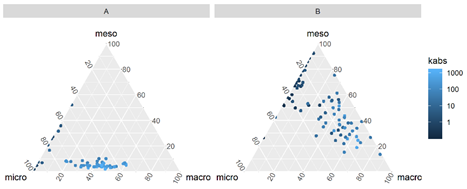
\includegraphics[width=0.75\linewidth]{figure/3-1-pchg-classes} 
  
  }
  
  \caption{Pore-throat class distribution for two sample reservoirs (A and B).}\label{fig:pchg-classes}
  \end{figure}
  \hypertarget{gauss-mixture-fit-feat}{%
  \subsection{Gaussian Mixture Fit Features}\label{gauss-mixture-fit-feat}}
  
  Following the methodology proposed by (Xu and Torres-Verdín \protect\hyperlink{ref-Xu2013}{2013}), bimodal gaussian mixture distributions, with parameters \(\mu_1\), \(\mu_2\), \(\sigma_1\), \(\sigma_2\), \(\lambda_1\) and \(\lambda_2\), were fitted to each MICP associated pore volume distributions \(p(\log{r})\), using the following approximation.
  \begin{equation} 
    p(\log{r}) \approx \lambda_1 \frac{1}{\sqrt{2\pi}\sigma_1}\exp{\frac{-(\log{r}-\mu_1)}{2\sigma_1^2}} + \lambda_2 \frac{1}{\sqrt{2\pi}\sigma_2}\exp{\frac{-(\log{r}-\mu_2)}{2\sigma_2^2}}
    \label{eq:gauss-mixture}
  \end{equation}
  \begin{equation} 
    \lambda_1 + \lambda_2 = 1 
    \label{eq:gauss-mixture-partition}
  \end{equation}
  The parameters \(\mu_1\), \(\mu_2\), \(\sigma_1\), \(\sigma_2\), \(\lambda_1\) and \(\lambda_2\), provide a compact representation of the MICP associated pore volume distributions \(p(\log{r})\), as exemplified in Figures \ref{fig:gauss-mixture-1} and \ref{fig:gauss-mixture-2}.
  \begin{figure}
  
  {\centering 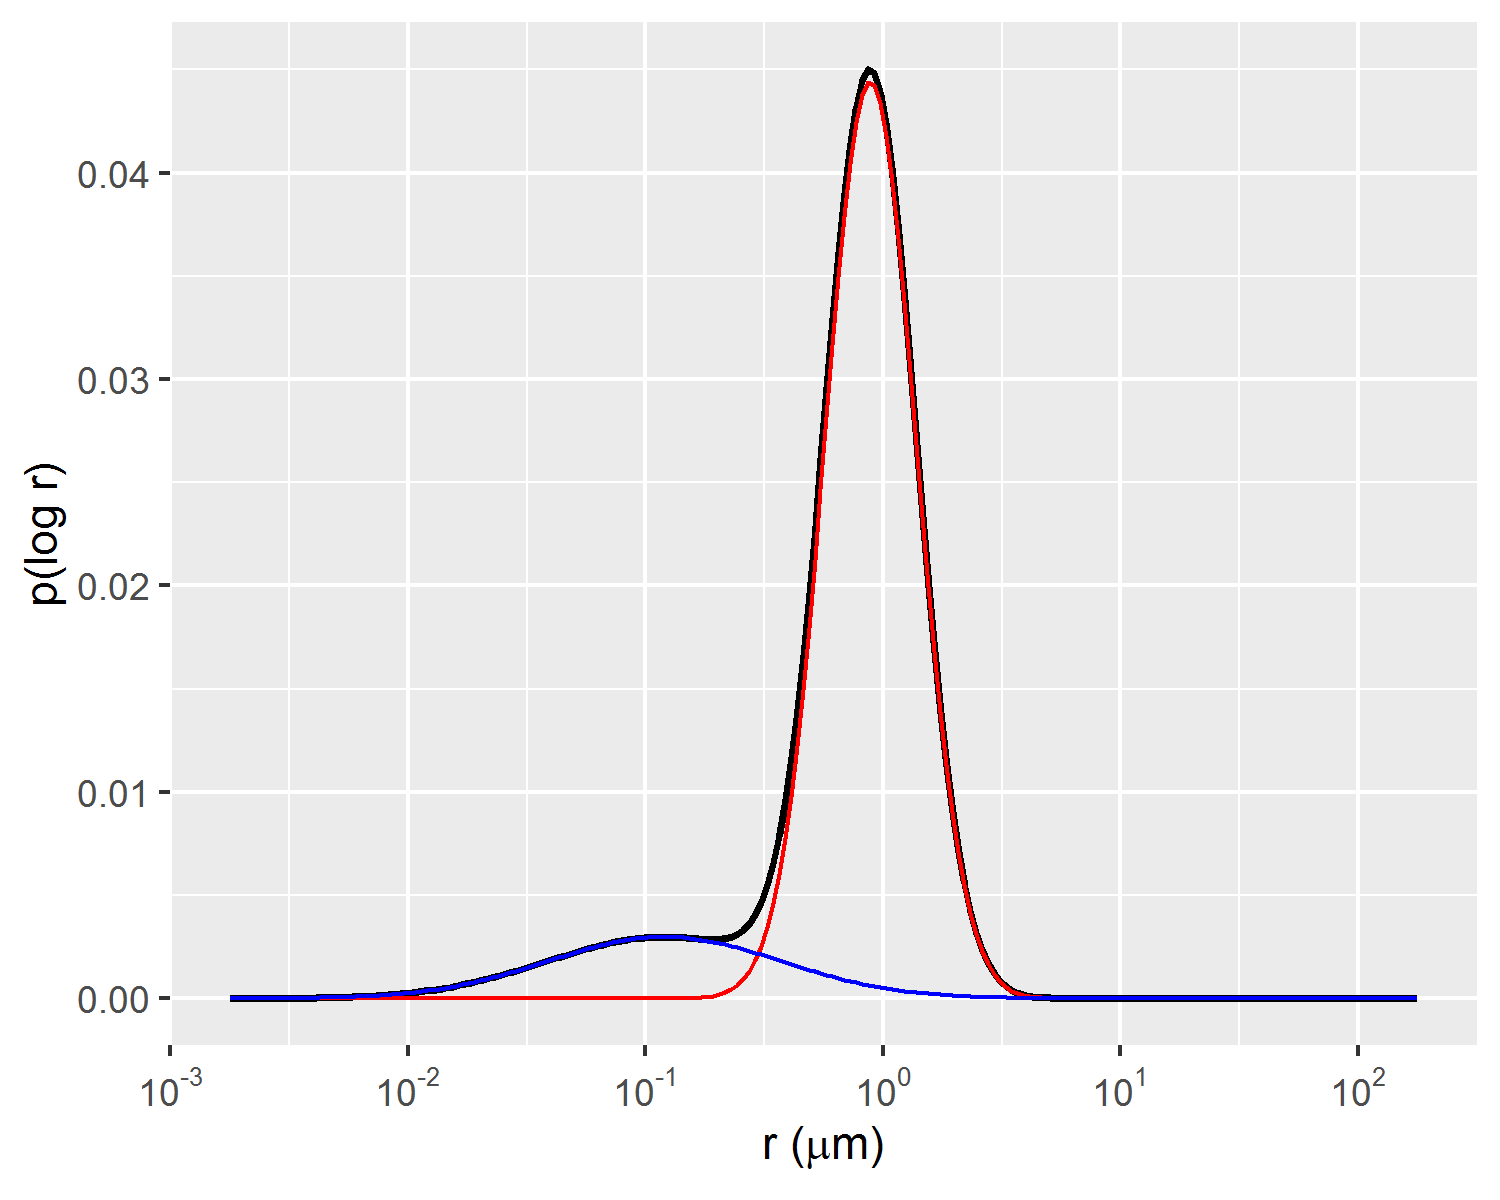
\includegraphics[width=0.75\linewidth]{figure/3-2-pchg-gauss-mixture-1} 
  
  }
  
  \caption{Example of bimodal gaussian mixture fit of p(log r) distribution.}\label{fig:gauss-mixture-1}
  \end{figure}
  \begin{figure}
  
  {\centering 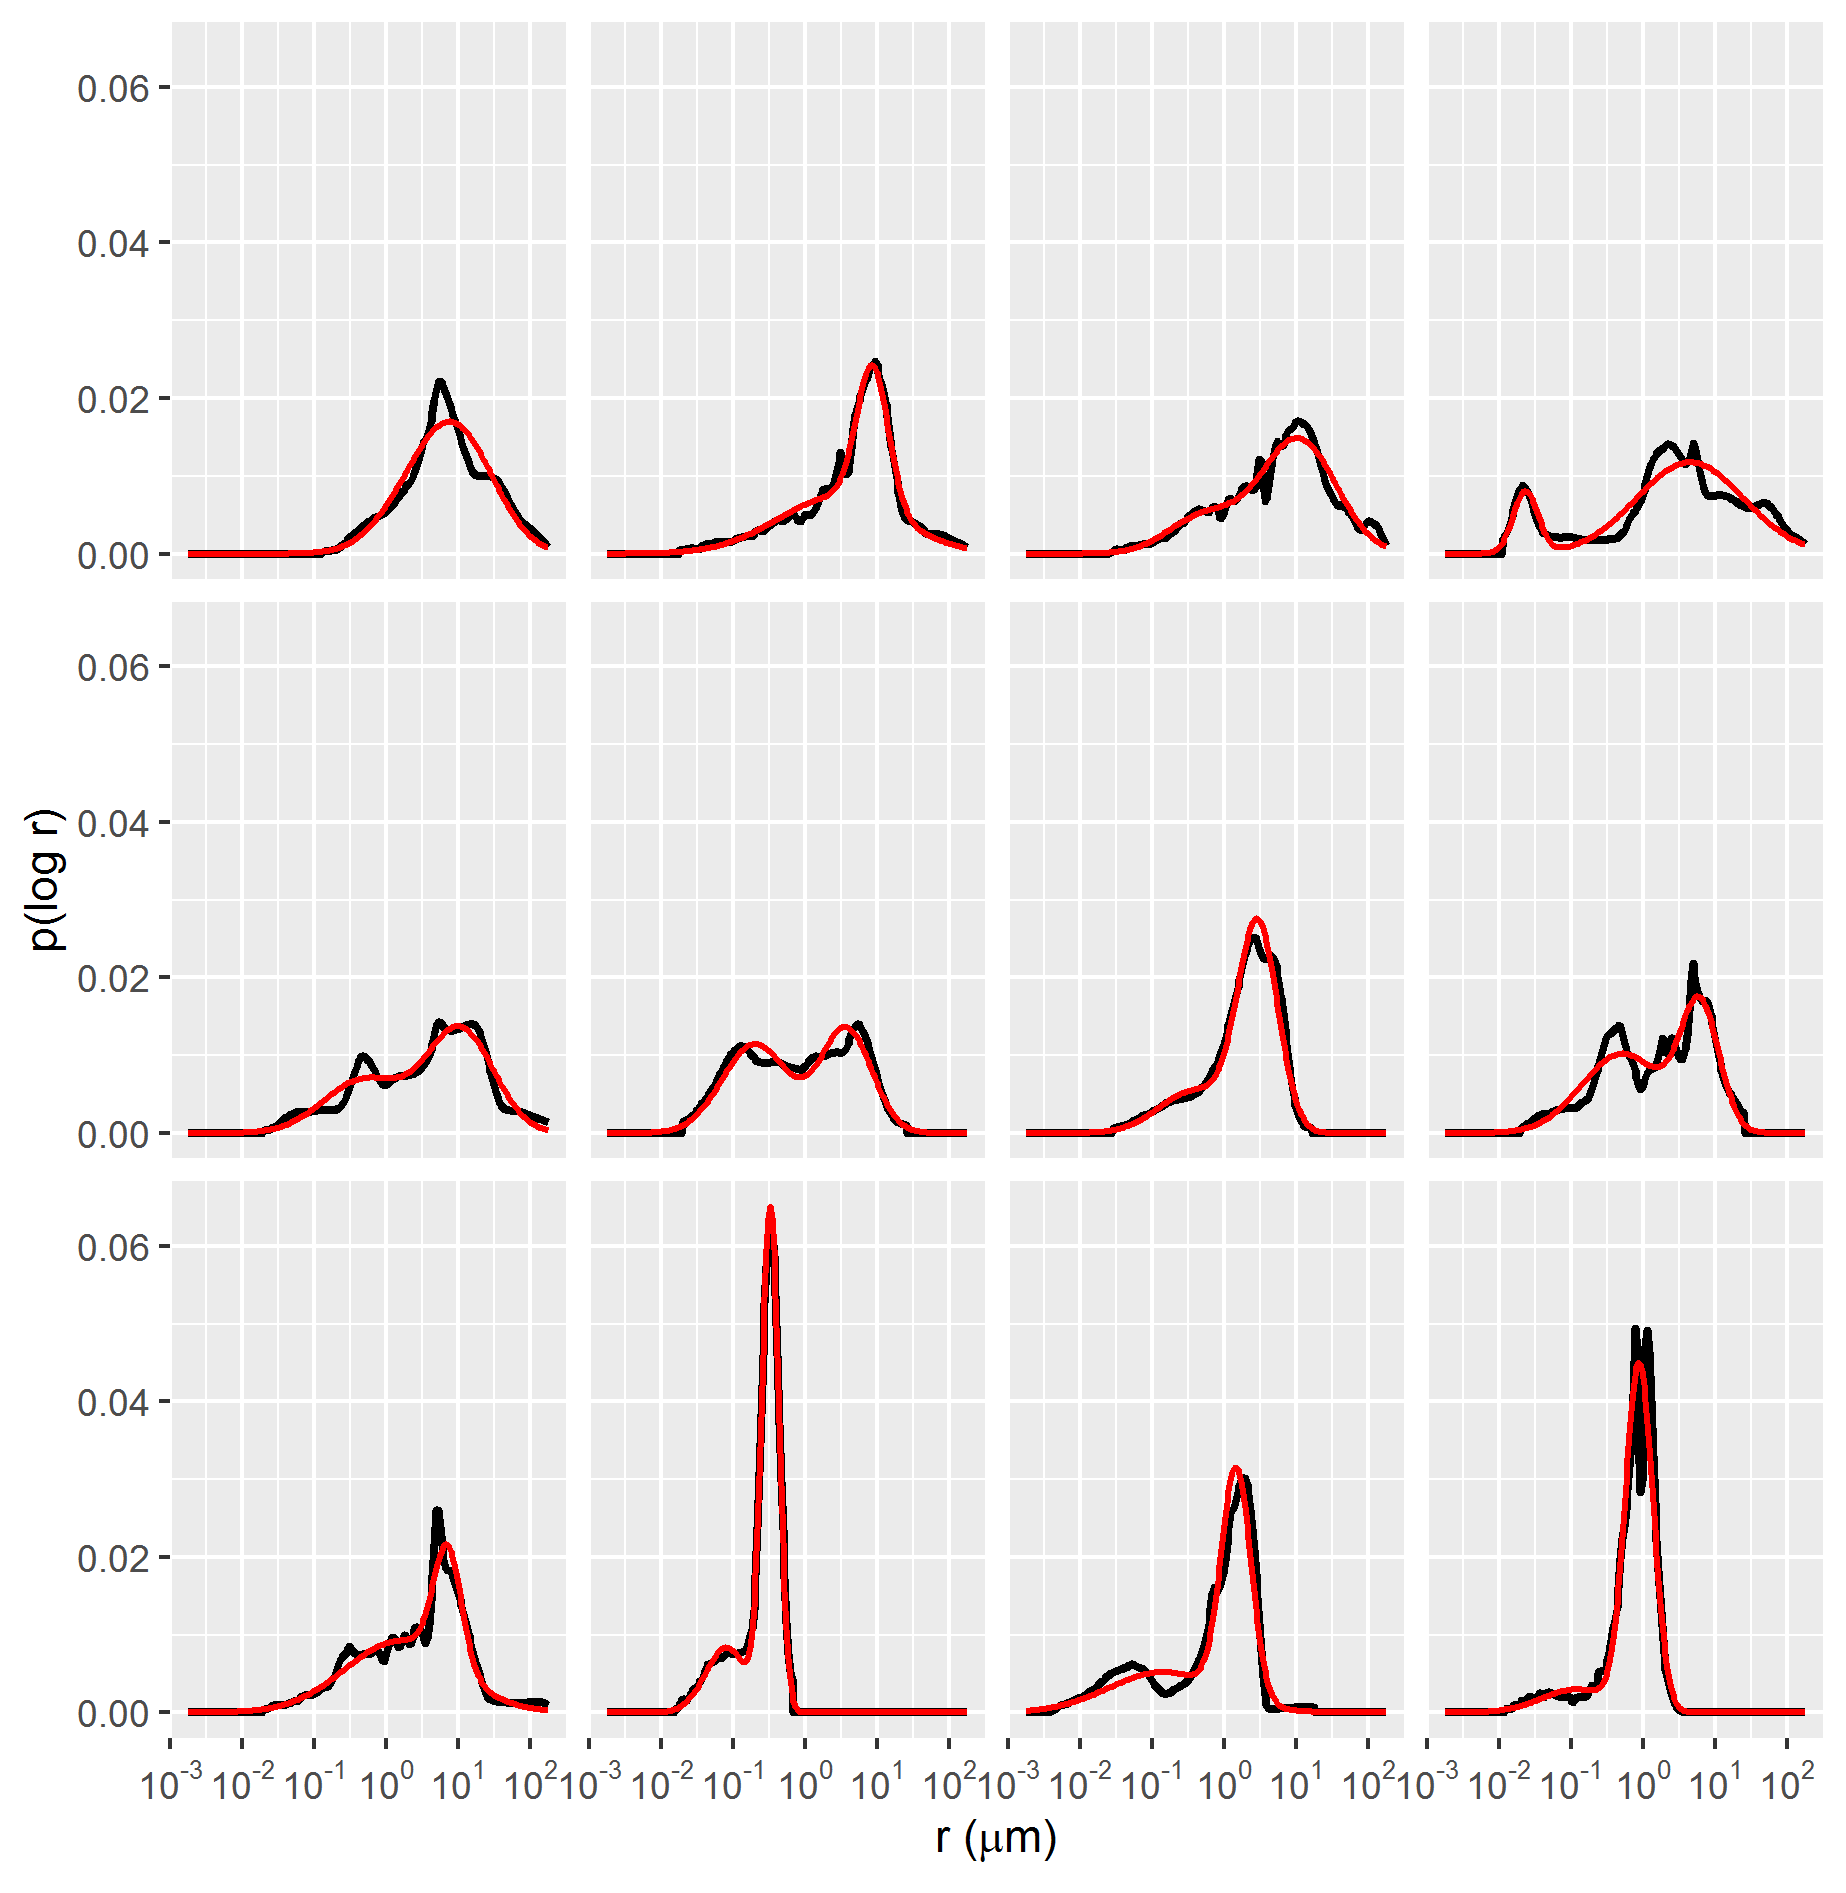
\includegraphics[width=0.75\linewidth]{figure/3-3-pchg-gauss-mixture-2} 
  
  }
  
  \caption{Gaussian mixture (red lines) fitted to p(log r) distributions of MICP data samples (black lines).}\label{fig:gauss-mixture-2}
  \end{figure}
  \hypertarget{dimensionality-reduction-features}{%
  \subsection{Dimensionality Reduction Features}\label{dimensionality-reduction-features}}
  
  Both linear and non-linear dimensionality reduction methods were used to extract features from the dataset of MICP curves. Dimensionality reduction techniques allow for the approximation of the dataset using a lower-dimensional representation, useful for data exploration and visualization and for data compression.
  
  Using as input pore-throat radius quantiles \{\(r_{15},r_{20},...,r_{85},r_{90}\)\}, the first two principal components PC1 and PC2 were estimated for each of the sample MICP curves using Principal Component Analysis (Hastie, Tibshirani, and Friedman \protect\hyperlink{ref-Hastie2009}{2009}). The first two principal components represented a total of 96.1\% of the variance in the dataset. A graphical depiction of the PC1 and PC2 features, colored by absolute permeability can be seen on Figure \ref{fig:pca-features}.
  
  The first and second principal components were shown to be correlated with absolute permeability \(k_{abs}\) and interquartile range \(iqr\), respectively, as displayed on Figures \ref{fig:pca-PC1} and \ref{fig:pca-PC2}.
  \begin{figure}[!ht]
  
  {\centering 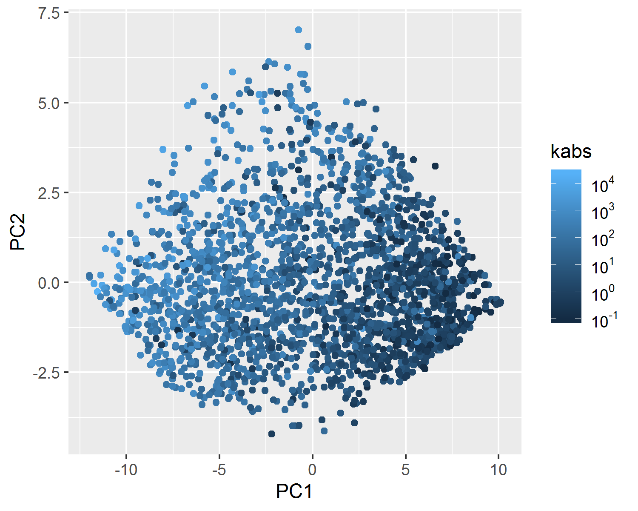
\includegraphics[width=0.75\linewidth]{figure/3-4-pca-features} 
  
  }
  
  \caption{First two principal components of each of the datasets MICP samples.}\label{fig:pca-features}
  \end{figure}
  \begin{figure}
  
  {\centering 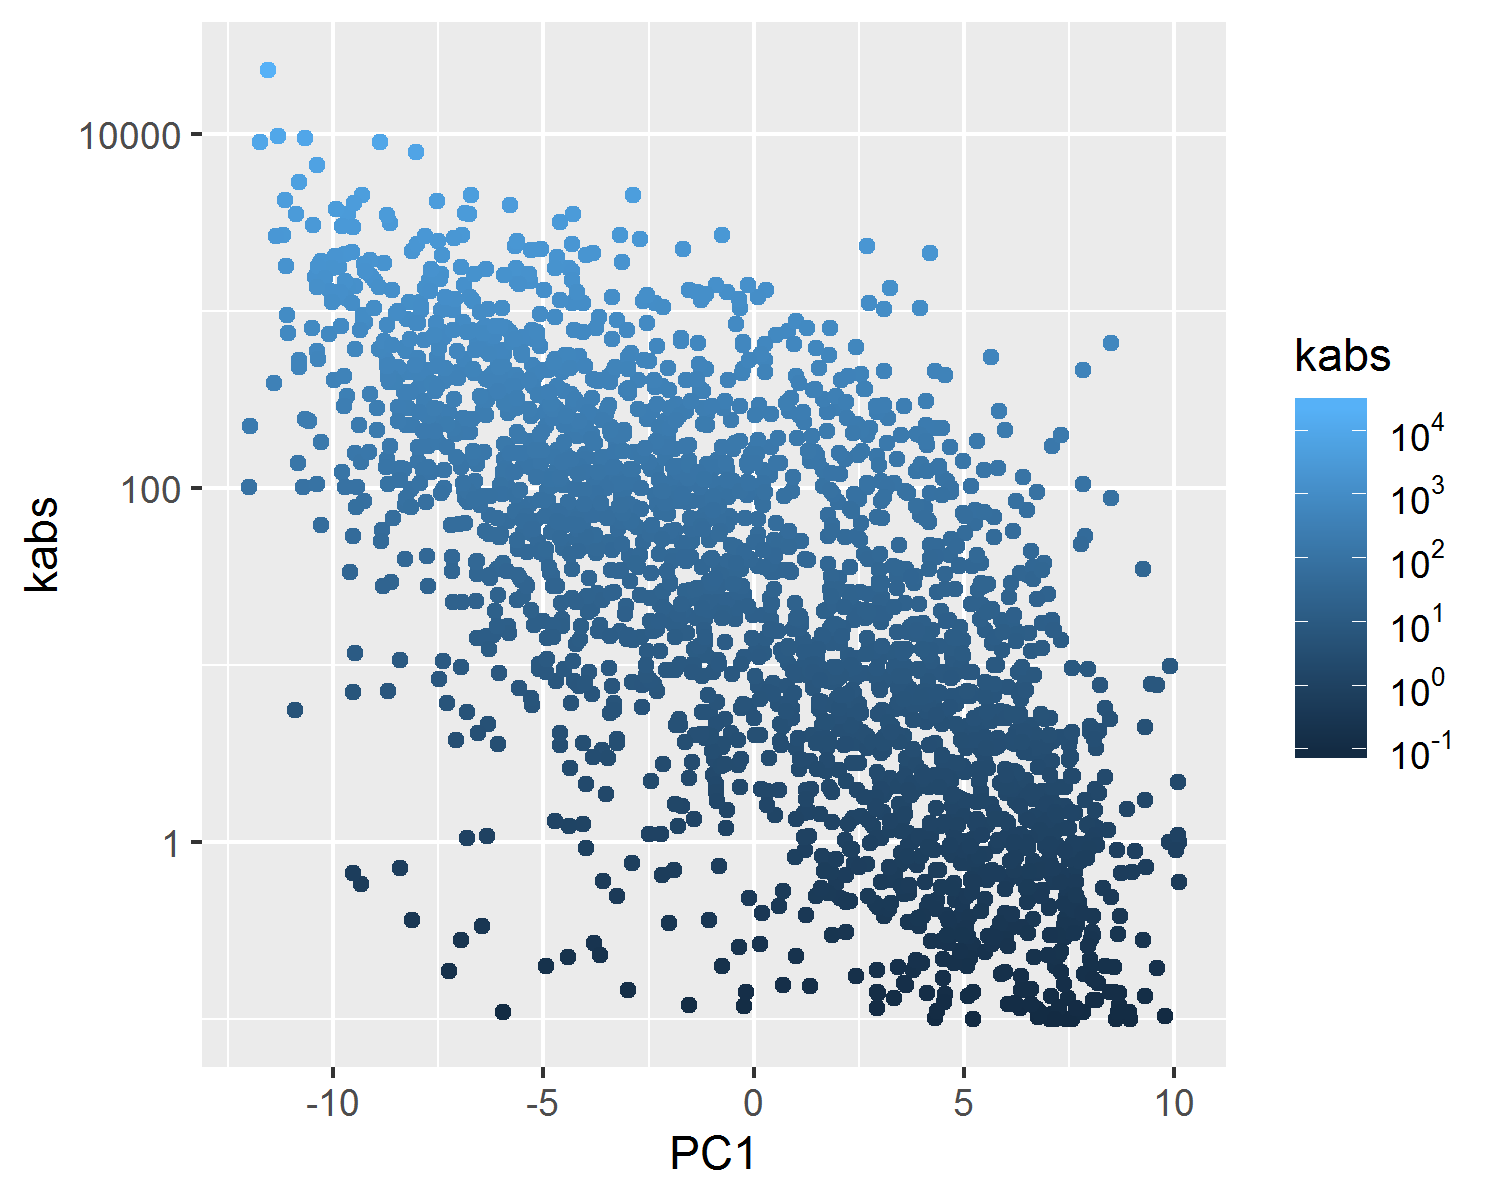
\includegraphics[width=0.75\linewidth]{figure/3-5-pca-PC1-kabs} 
  
  }
  
  \caption{Negative correlation between absolute permeability and the first principal component.}\label{fig:pca-PC1}
  \end{figure}
  \begin{figure}
  
  {\centering 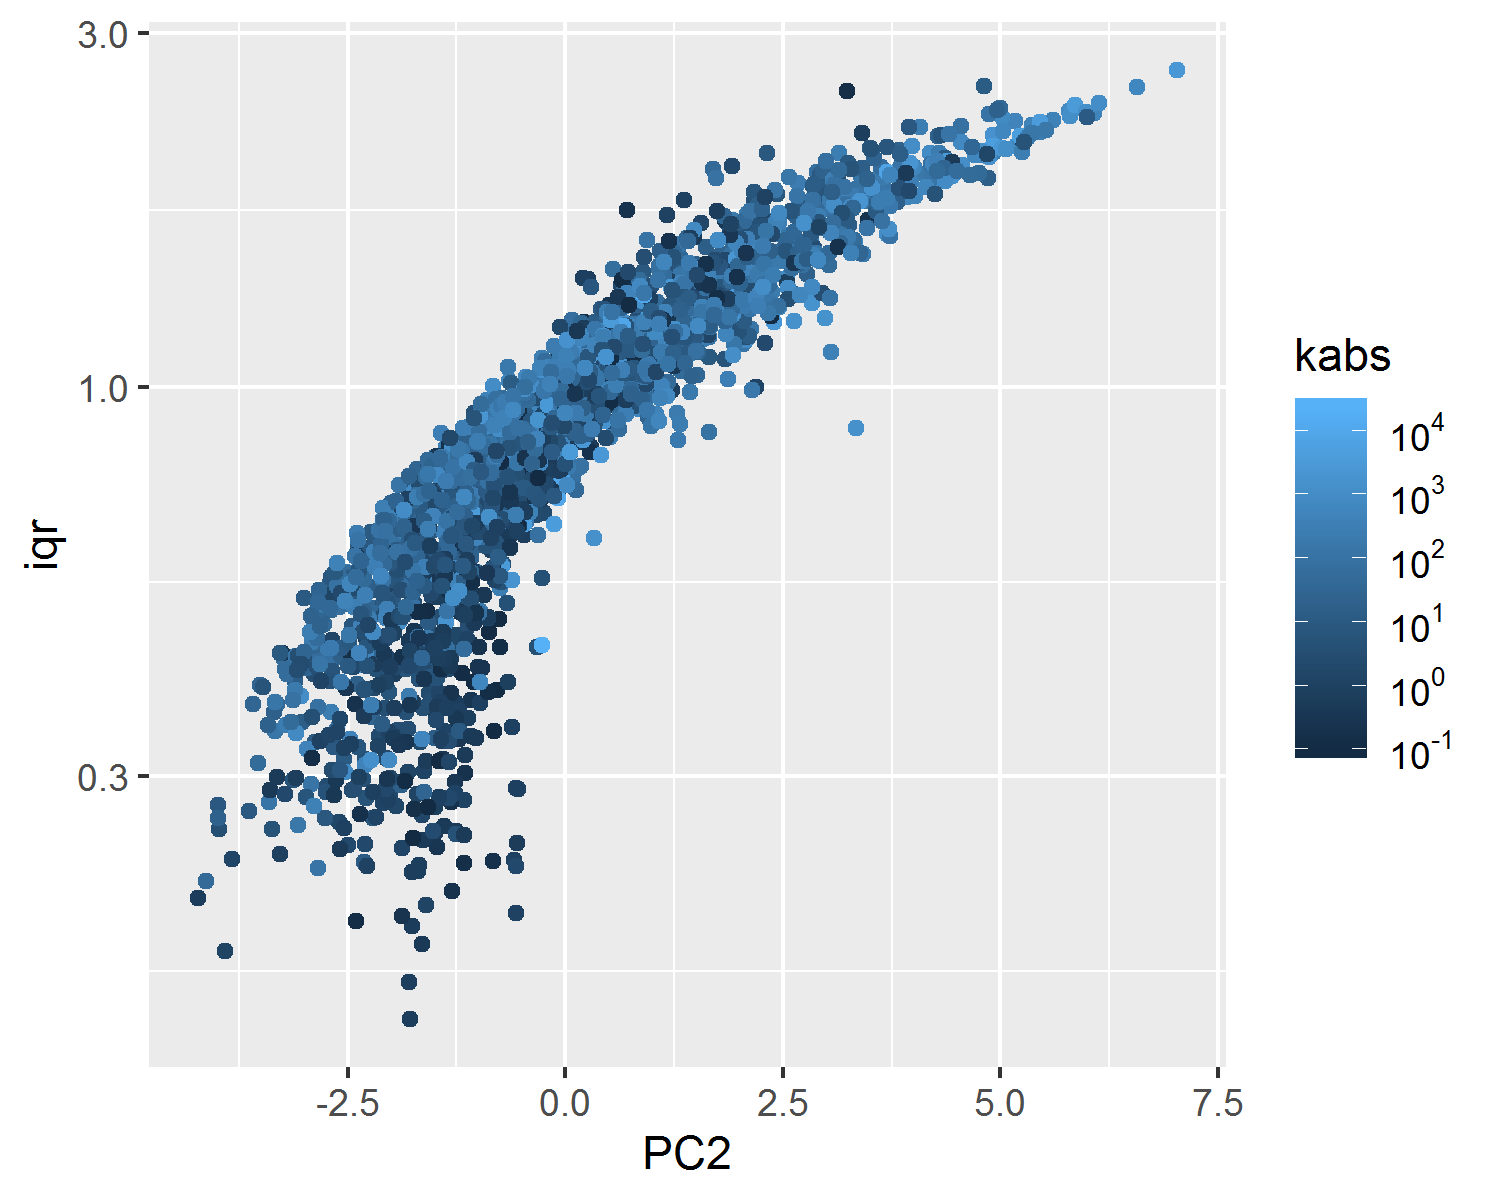
\includegraphics[width=0.75\linewidth]{figure/3-6-pca-PC2-iqr} 
  
  }
  
  \caption{Positive correlation between the interquartile-range iqr and the second principal component PC2.}\label{fig:pca-PC2}
  \end{figure}
  \par
  
  Non-linear dimensionality reduction features were also estimated using Uniform Manifold Approximation and Projection, also known as UMAP (McInnes and Healy \protect\hyperlink{ref-McInnes2018}{2018}), using as input pore-throat radius quantiles \{\(r_{15},r_{20},...,r_{85},r_{90}\)\}.
  \begin{figure}
  
  {\centering 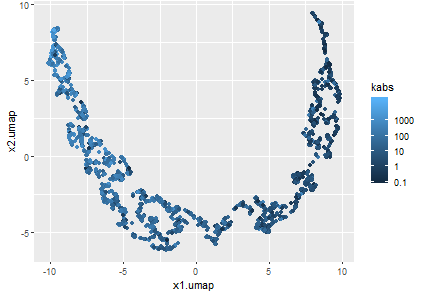
\includegraphics[width=0.75\linewidth]{figure/3-7-umap} 
  
  }
  
  \caption{MICP curves non-linear decomposition using UMAP.}\label{fig:umap}
  \end{figure}
  \par
  
  The Uniform Manifold Approximation and Projection technique constructs a high dimensional graph representation of the data and optimizes a low-dimensional manifold to be as structurally similar to the high dimensional graph as possible (McInnes and Healy \protect\hyperlink{ref-McInnes2018}{2018}). Due to its distance preserving properties, the low-dimensional manifold, represented in Figure \ref{fig:umap} by variables \(x_1.umap\) and \(x_2.umap\), is useful for visualization and identification of similar MICP curve samples.
  
  In Figure \ref{fig:umap-clustering}, this property is exemplified by a sequence of three pairs of plots, showing that samples mapped to the same regions of the UMAP manifold, marked in the red in each of the plot pairs, correspond to distributions \(p(\log{r})\) with similar characteristics.
  \begin{figure}[!h]
  
  {\centering 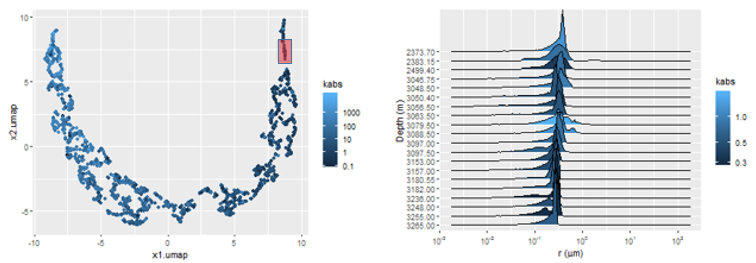
\includegraphics[width=0.9\linewidth]{figure/3-8-umap-I} 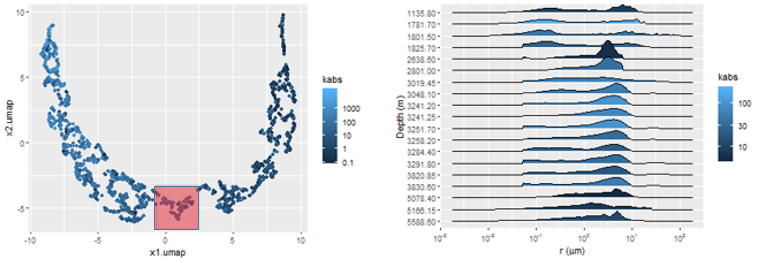
\includegraphics[width=0.9\linewidth]{figure/3-8-umap-II} 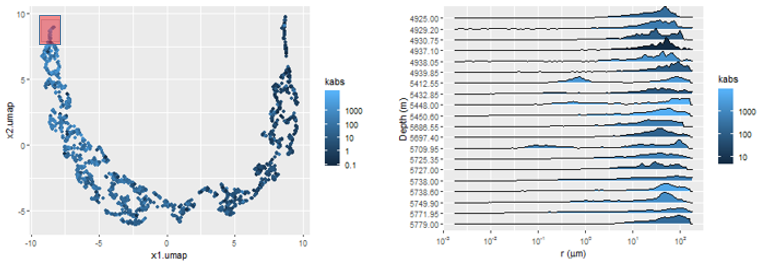
\includegraphics[width=0.9\linewidth]{figure/3-8-umap-III} 
  
  }
  
  \caption{Manifold maps (left) showing areas with similar associated pore volume distributions p(log r) (right).}\label{fig:umap-clustering}
  \end{figure}
  \hypertarget{absolute-permeability-regression-models}{%
  \section{Absolute Permeability Regression Models}\label{absolute-permeability-regression-models}}
  
  The regression metrics root mean squared error \eqref{eq:RMSE}, median absolute error \eqref{eq:MAE} and \(R^2\) \eqref{eq:R2} were evaluated for the trained regression models. Due to the issues regarding the representativeness of the rock fragments with respect to the measured absolute permeability values, discussed on chapter \ref{petrophysical-properties}, minimization of the median absolute deviation metric \eqref{eq:MAE} was chosen to increase the robustness to outliers of the trained non-linear regression models, described in section \ref{non-linear-regression}. In both linear and non-linear regression methods, the \(R^2\) metric \eqref{eq:R2} was used for further assessment of the trained regression models.
  \begin{equation} 
    \text{RMSE} = \sqrt{\frac{\sum_{i=1}^n{(\log{\hat{k}_{{abs}_i}}-\log{k_{{abs}_i}})^2}}{n}}
    \label{eq:RMSE}
  \end{equation}
  \begin{equation} 
    \text{MAE} = \frac{\sum_{i=1}^n{|\log{\hat{k}_{{abs}_i}}-\log{k_{{abs}_i}}}|}{n}
    \label{eq:MAE}
  \end{equation}
  \begin{equation} 
    R^2 = 1-\frac{\sum_{i=1}^n{(\log{\hat{k}_{{abs}_i}}-\log{k_{{abs}_i}})^2}}{\sum_{i=1}^n{(\log{k_{{abs}_i}}-\overline{\log{k_{{abs}_i}}})^2}}
    \label{eq:R2}
  \end{equation}
  \hypertarget{linear-regression-models}{%
  \subsection{Linear Regression Models}\label{linear-regression-models}}
  
  The linear features, described in section \ref{linear-features}, were used to fit linear regression logarithmic absolute permeability \(\log{k_{abs}}\) models.
  
  Among the fitted linear regression models, the Winland and Swanson models obtained the lowest root mean squared error and highest coefficient of determination metrics.
  
  Figure \ref{fig:linear-models} shows a graphical representation of the fitted models, where a significant number of outlier logarithmic absolute permeability estimates \(\log{\hat{k}_{abs}}\) , with more than one order of magnitude errors, can be seen. The presence of this large number of outliers can be explained by the limited rock fragment representativeness of the core sample pore volume for heterogeneous reservoirs, described in chapter \ref{petrophysical-properties}.
  \begin{figure}
  
  {\centering 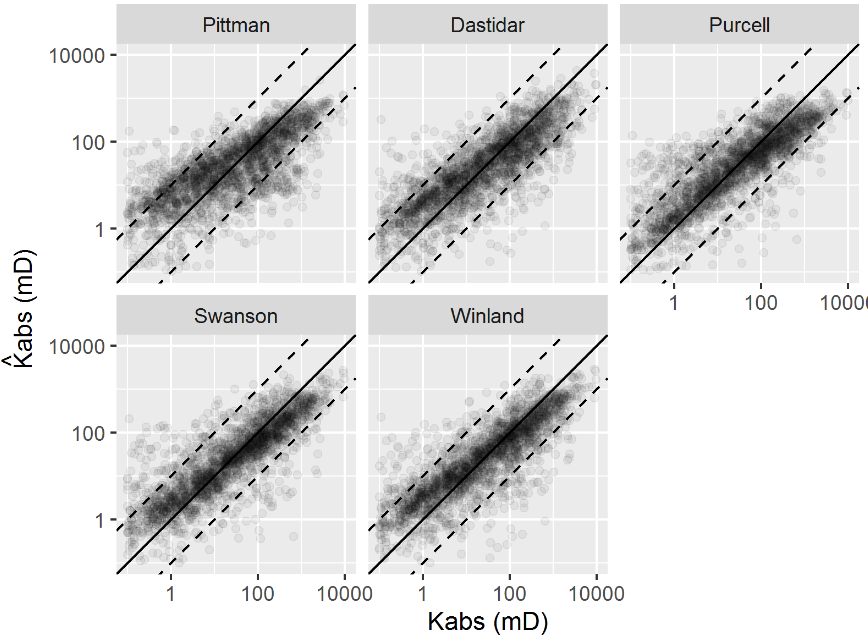
\includegraphics[width=0.75\linewidth]{figure/3-9-linear-models} 
  
  }
  
  \caption{Visual evaluation of the predicted and observed absolute permeability models using linear features.}\label{fig:linear-models}
  \end{figure}
  \begin{figure}
  
  {\centering 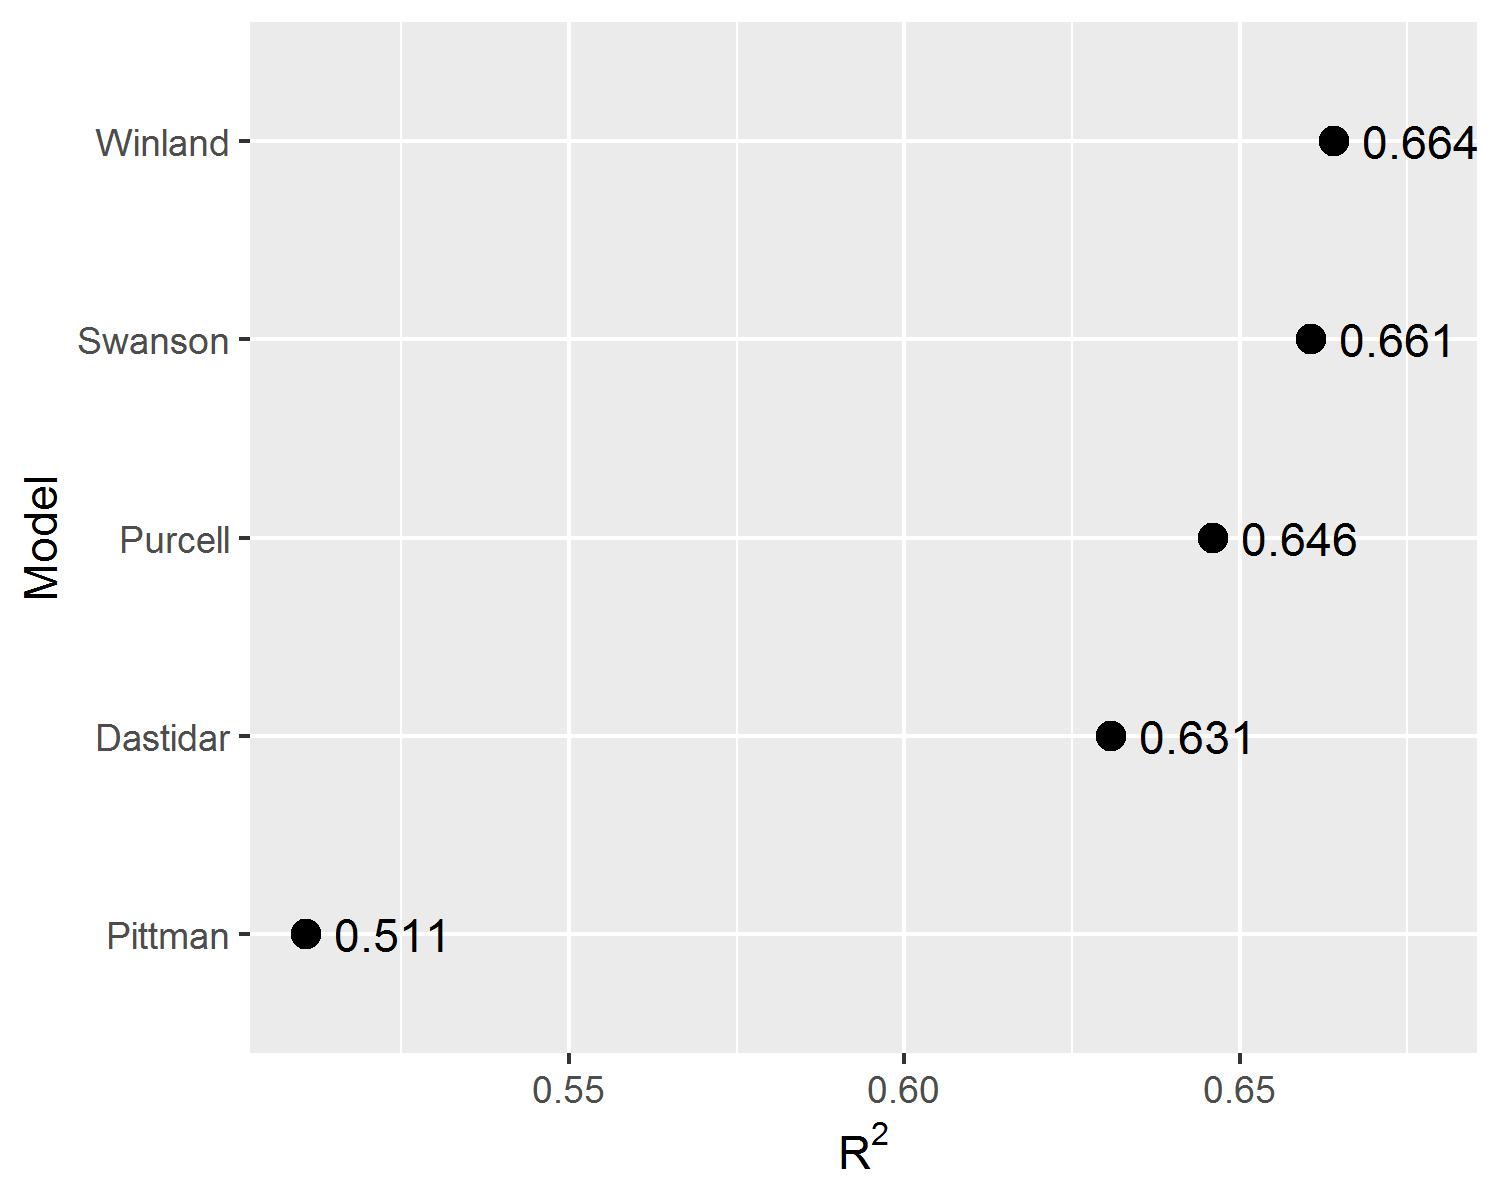
\includegraphics[width=0.75\linewidth]{figure/3-10-linear-models-R2} 
  
  }
  
  \caption{Comparison of the $R^2$ metric for the fitted linear regression models.}\label{fig:linear-models-R2}
  \end{figure}
  \hypertarget{non-linear-regression}{%
  \subsection{Black-Box Machine Learning Models}\label{non-linear-regression}}
  
  Using the features described in section \ref{pchg-feat-eng}, six additional non-linear regression models were fit to the dataset using machine learning models. The 2324 MICP curves were split between training and test data, with a eighty to twenty percent ratio. Using the training set, each algorithm went through a hyper-parameter tuning procedure, using ten times repeated five-fold cross-validation error estimation, on a grid of selected hyper-parameters.
  
  Two \(knn\) nearest neighbors models (P. Murphy \protect\hyperlink{ref-P.Murphy2012}{2012}), were fit to the training set, one using features extracted using PCA (Hastie, Tibshirani, and Friedman \protect\hyperlink{ref-Hastie2009}{2009}) and the other features extracted using UMAP non-linear dimensionality reduction (McInnes and Healy \protect\hyperlink{ref-McInnes2018}{2018}).
  
  A simple linear regression model was fit using the features extracted from the bi-modal gaussian mixture model proposed by (Xu and Torres-Verdín \protect\hyperlink{ref-Xu2013}{2013}), described in section \ref{gauss-mixture-fit-feat}.
  
  A support vector regression (SVR) model, a random forest model and a gradient boosted trees model (Hastie, Tibshirani, and Friedman \protect\hyperlink{ref-Hastie2009}{2009}) were fit to an expanded feature set, consisting of the features proposed by Swanson, Winland, Purcell, the sample porosity \(\phi\), the micropores and mesopores ternary class distributions, the UMAP features and the bi-modal gaussian mixtures distribution features. A pre-processing standardizing step was applied to each feature. The gradient boosted trees model was fitted using the implementation provided by the XGBoost library (Chen and Guestrin \protect\hyperlink{ref-Chen2016}{2016}).
  \begin{figure}
  
  {\centering 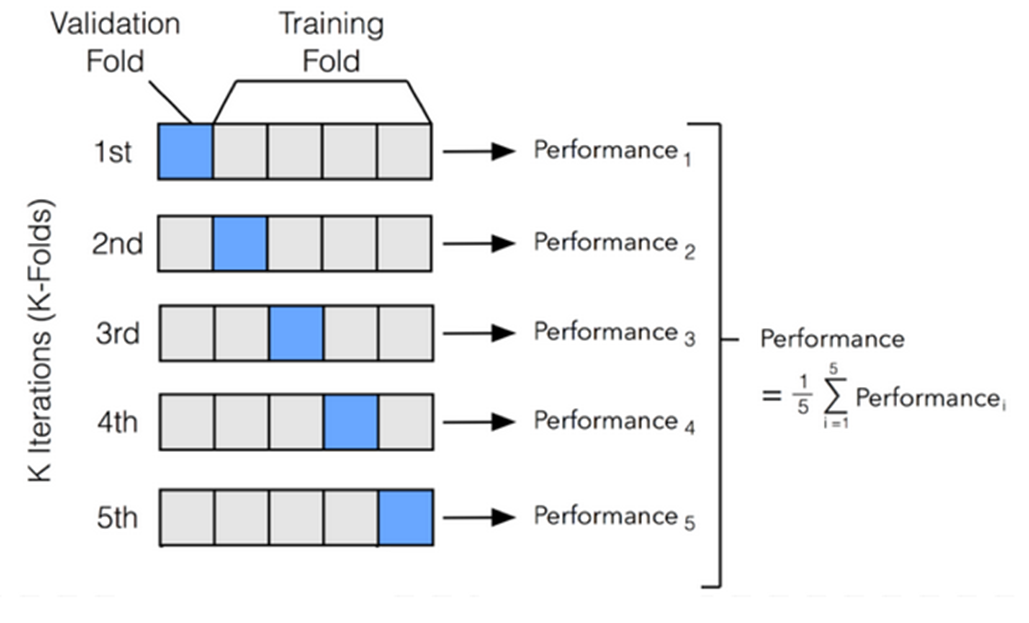
\includegraphics[width=0.7\linewidth]{figure/3-11-cross-validation} 
  
  }
  
  \caption{Five-fold cross-validation procedure.}\label{fig:cross-validation}
  \end{figure}
  \par
  
  Table \ref{tab:regression-metrics} and Figure \ref{fig:cross-validation-metrics} show median values of repeated five-fold cross-validated MAE, \(R^2\) and RMSE metrics for each of the trained regression models. The regression models with the lowest median absolute error were the SVR, randomForest and gradient boosted trees XGB models. Through the use of a radial basis function kernel and an optimization procedure that minimizes hinge loss (Hastie, Tibshirani, and Friedman \protect\hyperlink{ref-Hastie2009}{2009}), the SVR algorithm provides outlier robust predictions. The random forest and gradient boosted trees algorithms use randomized selection of features and data subsets, bagging and boosting techniques, respectively, to reduce prediction errors of ensembles of simpler decision tree models (Chen and Guestrin \protect\hyperlink{ref-Chen2016}{2016}).
  \begin{longtable}[]{@{}cccc@{}}
  \caption{\label{tab:regression-metrics} Median repeated five-fold cross-validated MAE, \(R^2\) and RMSE metrics for each model.}\tabularnewline
  \toprule
  \begin{minipage}[b]{0.26\columnwidth}\centering
  Regression Model\strut
  \end{minipage} & \begin{minipage}[b]{0.10\columnwidth}\centering
  MAE\strut
  \end{minipage} & \begin{minipage}[b]{0.10\columnwidth}\centering
  \(R^2\)\strut
  \end{minipage} & \begin{minipage}[b]{0.10\columnwidth}\centering
  RMSE\strut
  \end{minipage}\tabularnewline
  \midrule
  \endfirsthead
  \toprule
  \begin{minipage}[b]{0.26\columnwidth}\centering
  Regression Model\strut
  \end{minipage} & \begin{minipage}[b]{0.10\columnwidth}\centering
  MAE\strut
  \end{minipage} & \begin{minipage}[b]{0.10\columnwidth}\centering
  \(R^2\)\strut
  \end{minipage} & \begin{minipage}[b]{0.10\columnwidth}\centering
  RMSE\strut
  \end{minipage}\tabularnewline
  \midrule
  \endhead
  \begin{minipage}[t]{0.26\columnwidth}\centering
  SVR\strut
  \end{minipage} & \begin{minipage}[t]{0.10\columnwidth}\centering
  0.412\strut
  \end{minipage} & \begin{minipage}[t]{0.10\columnwidth}\centering
  0.722\strut
  \end{minipage} & \begin{minipage}[t]{0.10\columnwidth}\centering
  0.596\strut
  \end{minipage}\tabularnewline
  \begin{minipage}[t]{0.26\columnwidth}\centering
  randomForest\strut
  \end{minipage} & \begin{minipage}[t]{0.10\columnwidth}\centering
  0.437\strut
  \end{minipage} & \begin{minipage}[t]{0.10\columnwidth}\centering
  0.712\strut
  \end{minipage} & \begin{minipage}[t]{0.10\columnwidth}\centering
  0.604\strut
  \end{minipage}\tabularnewline
  \begin{minipage}[t]{0.26\columnwidth}\centering
  XGB\strut
  \end{minipage} & \begin{minipage}[t]{0.10\columnwidth}\centering
  0.439\strut
  \end{minipage} & \begin{minipage}[t]{0.10\columnwidth}\centering
  0.711\strut
  \end{minipage} & \begin{minipage}[t]{0.10\columnwidth}\centering
  0.605\strut
  \end{minipage}\tabularnewline
  \begin{minipage}[t]{0.26\columnwidth}\centering
  Swanson\strut
  \end{minipage} & \begin{minipage}[t]{0.10\columnwidth}\centering
  0.471\strut
  \end{minipage} & \begin{minipage}[t]{0.10\columnwidth}\centering
  0.681\strut
  \end{minipage} & \begin{minipage}[t]{0.10\columnwidth}\centering
  0.639\strut
  \end{minipage}\tabularnewline
  \begin{minipage}[t]{0.26\columnwidth}\centering
  GaussianMixture\strut
  \end{minipage} & \begin{minipage}[t]{0.10\columnwidth}\centering
  0.477\strut
  \end{minipage} & \begin{minipage}[t]{0.10\columnwidth}\centering
  0.675\strut
  \end{minipage} & \begin{minipage}[t]{0.10\columnwidth}\centering
  0.641\strut
  \end{minipage}\tabularnewline
  \begin{minipage}[t]{0.26\columnwidth}\centering
  Winland\strut
  \end{minipage} & \begin{minipage}[t]{0.10\columnwidth}\centering
  0.481\strut
  \end{minipage} & \begin{minipage}[t]{0.10\columnwidth}\centering
  0.674\strut
  \end{minipage} & \begin{minipage}[t]{0.10\columnwidth}\centering
  0.643\strut
  \end{minipage}\tabularnewline
  \begin{minipage}[t]{0.26\columnwidth}\centering
  Purcell\strut
  \end{minipage} & \begin{minipage}[t]{0.10\columnwidth}\centering
  0.487\strut
  \end{minipage} & \begin{minipage}[t]{0.10\columnwidth}\centering
  0.661\strut
  \end{minipage} & \begin{minipage}[t]{0.10\columnwidth}\centering
  0.654\strut
  \end{minipage}\tabularnewline
  \begin{minipage}[t]{0.26\columnwidth}\centering
  Dastidar\strut
  \end{minipage} & \begin{minipage}[t]{0.10\columnwidth}\centering
  0.520\strut
  \end{minipage} & \begin{minipage}[t]{0.10\columnwidth}\centering
  0.642\strut
  \end{minipage} & \begin{minipage}[t]{0.10\columnwidth}\centering
  0.673\strut
  \end{minipage}\tabularnewline
  \begin{minipage}[t]{0.26\columnwidth}\centering
  knnUMAP\strut
  \end{minipage} & \begin{minipage}[t]{0.10\columnwidth}\centering
  0.565\strut
  \end{minipage} & \begin{minipage}[t]{0.10\columnwidth}\centering
  0.562\strut
  \end{minipage} & \begin{minipage}[t]{0.10\columnwidth}\centering
  0.744\strut
  \end{minipage}\tabularnewline
  \begin{minipage}[t]{0.26\columnwidth}\centering
  knnPCA\strut
  \end{minipage} & \begin{minipage}[t]{0.10\columnwidth}\centering
  0.581\strut
  \end{minipage} & \begin{minipage}[t]{0.10\columnwidth}\centering
  0.547\strut
  \end{minipage} & \begin{minipage}[t]{0.10\columnwidth}\centering
  0.753\strut
  \end{minipage}\tabularnewline
  \begin{minipage}[t]{0.26\columnwidth}\centering
  Pittman\strut
  \end{minipage} & \begin{minipage}[t]{0.10\columnwidth}\centering
  0.613\strut
  \end{minipage} & \begin{minipage}[t]{0.10\columnwidth}\centering
  0.523\strut
  \end{minipage} & \begin{minipage}[t]{0.10\columnwidth}\centering
  0.775\strut
  \end{minipage}\tabularnewline
  \bottomrule
  \end{longtable}
  \begin{figure}
  
  {\centering 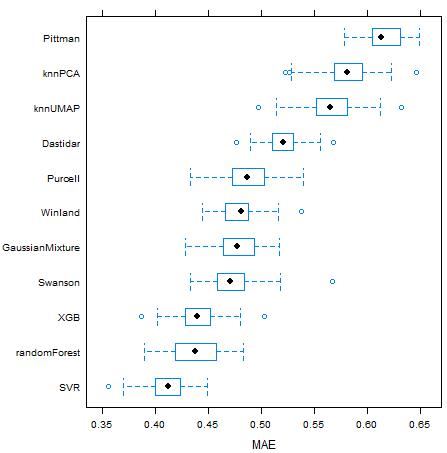
\includegraphics[width=0.75\linewidth]{figure/3-12-cross-validation-MAE} 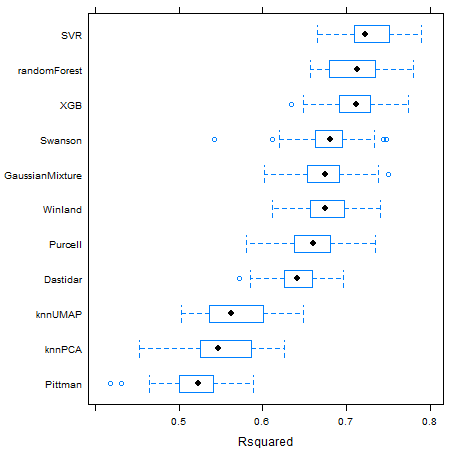
\includegraphics[width=0.75\linewidth]{figure/3-12-cross-validation-R2} 
  
  }
  
  \caption{Boxplots for repeated five-fold cross-validated MAE, $R^2$ and RMSE metric results for each model.}\label{fig:cross-validation-metrics}
  \end{figure}
  Non-linear machine learning models presented consistently lower prediction errors, as can be seen on Figure \ref{fig:cross-validation-metrics}. On Figure \ref{fig:cross-validation-models}, a visual comparison between linear and non-linear machine learning models of the predicted versus measured data for the test dataset is shown. Although the non-linear machine-learning models did obtain better MAE, \(R^2\) and RMSE metrics results, a significant number of outliers are still present, probably related to the issue of limited rock fragment representativeness of highly heterogeneous reservoirs described in chapter \ref{petrophysical-properties}.
  \begin{figure}[t]
  
  {\centering 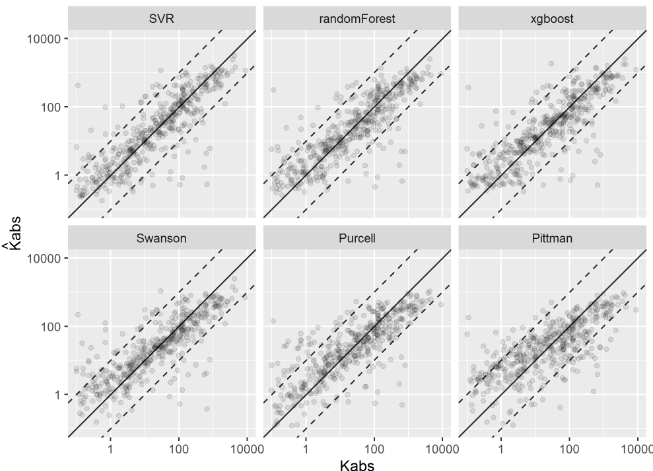
\includegraphics[width=0.9\linewidth]{figure/3-13-cross-validation-models} 
  
  }
  
  \caption{Visual evaluation of the estimated absolute permeability models using Machine Learning and linear models.}\label{fig:cross-validation-models}
  \end{figure}
  \hypertarget{hierarchical-linear-regression}{%
  \chapter{Hierarchical Multi-Task Linear Regression}\label{hierarchical-linear-regression}}
  
  Linear regression methods are widely used in petrophysical characterization. Compared to non-linear machine learning models, they have as advantages simplicity, interpretability and their inherent linear behavior on extrapolated predictions. For the estimation of special core analysis properties, which are costly to acquire and thus usually scarce, simple models with a low number of parameters and that can deliver interpretable probabilistic inferences are highly desirable. In this work, two different linear regression techniques are evaluated on special core analysis datasets.
  
  On a dataset containing 135 capillary pressure curves estimated from centrifuge experiments, a multi-task linear regression model is fit and evaluated, and some of its properties are analyzed.
  
  On another dataset, containing 226 unsteady-state water-oil relative permeability curves, partially pooled hierarchical linear regression models are evaluated and compared to simple linear regression models.
  
  \hypertarget{multi-task-linear-regression}{%
  \section{Multi-Task Linear Regression}\label{multi-task-linear-regression}}
  
  Using the parameterization \eqref{eq:albu2}, proposed by (Albuquerque et al. \protect\hyperlink{ref-Albuquerque2018}{2018}), a dataset containing parameters \(S_{wi}\), \(P_e\), \(\alpha\) and \(\beta\) fitted to each of the available 135 centrifuge capillary pressure curves, was assembled.
  \begin{equation} 
    S_w(P_c, S_{wi}, P_e, \alpha, \beta) = \frac{1+\alpha S_{wi}(P_c - P_e)^\beta}{(1+\alpha (P_c - P_e)^\beta}
    \label{eq:albu2}
  \end{equation}
  To each of these samples, features extracted from MICP curves obtained on corresponding rock fragments were associated in a dataset containing \{\(S_{wi}\), \(P_e\), \(\alpha\), \(\beta\), \(k_{abs}\), \(r_{35}\), \(iqr\)\} values for each MICP and centrifuge capillary pressure curve pair. Significant correlations between corresponding centrifuge capillary pressure curves \(\alpha\), \(S_{wi}\) and MICP median pore throat radius \(r_{median}\) parameters can be visualized in Figure \ref{fig:pcc-correlations2}.
  \begin{figure}
  
  {\centering 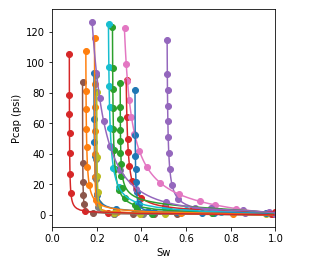
\includegraphics[width=0.7\linewidth]{figure/2-9-pcc-dataset} 
  
  }
  
  \caption{Sample of the experimental capillary pressure curve dataset (points) and fitted capillary pressure model (lines).}\label{fig:pcc-dataset2}
  \end{figure}
  \begin{figure}
  
  {\centering 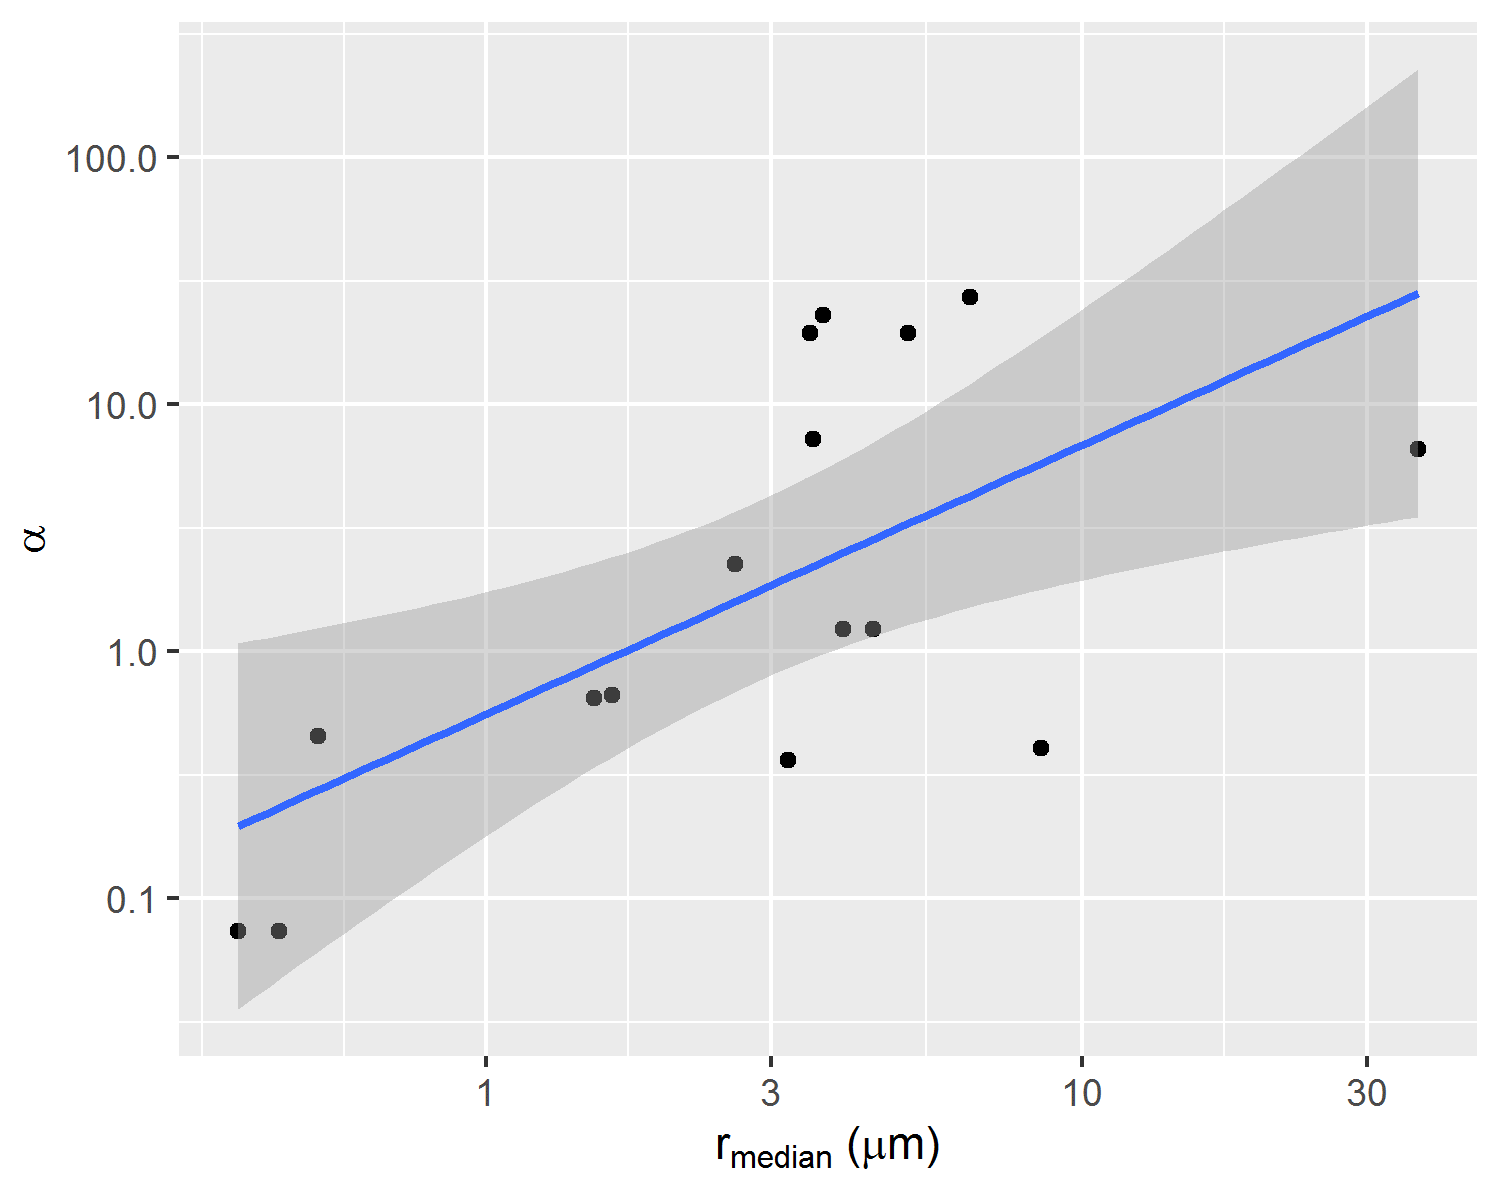
\includegraphics[width=0.45\linewidth]{figure/2-12a-correlations-pchg} 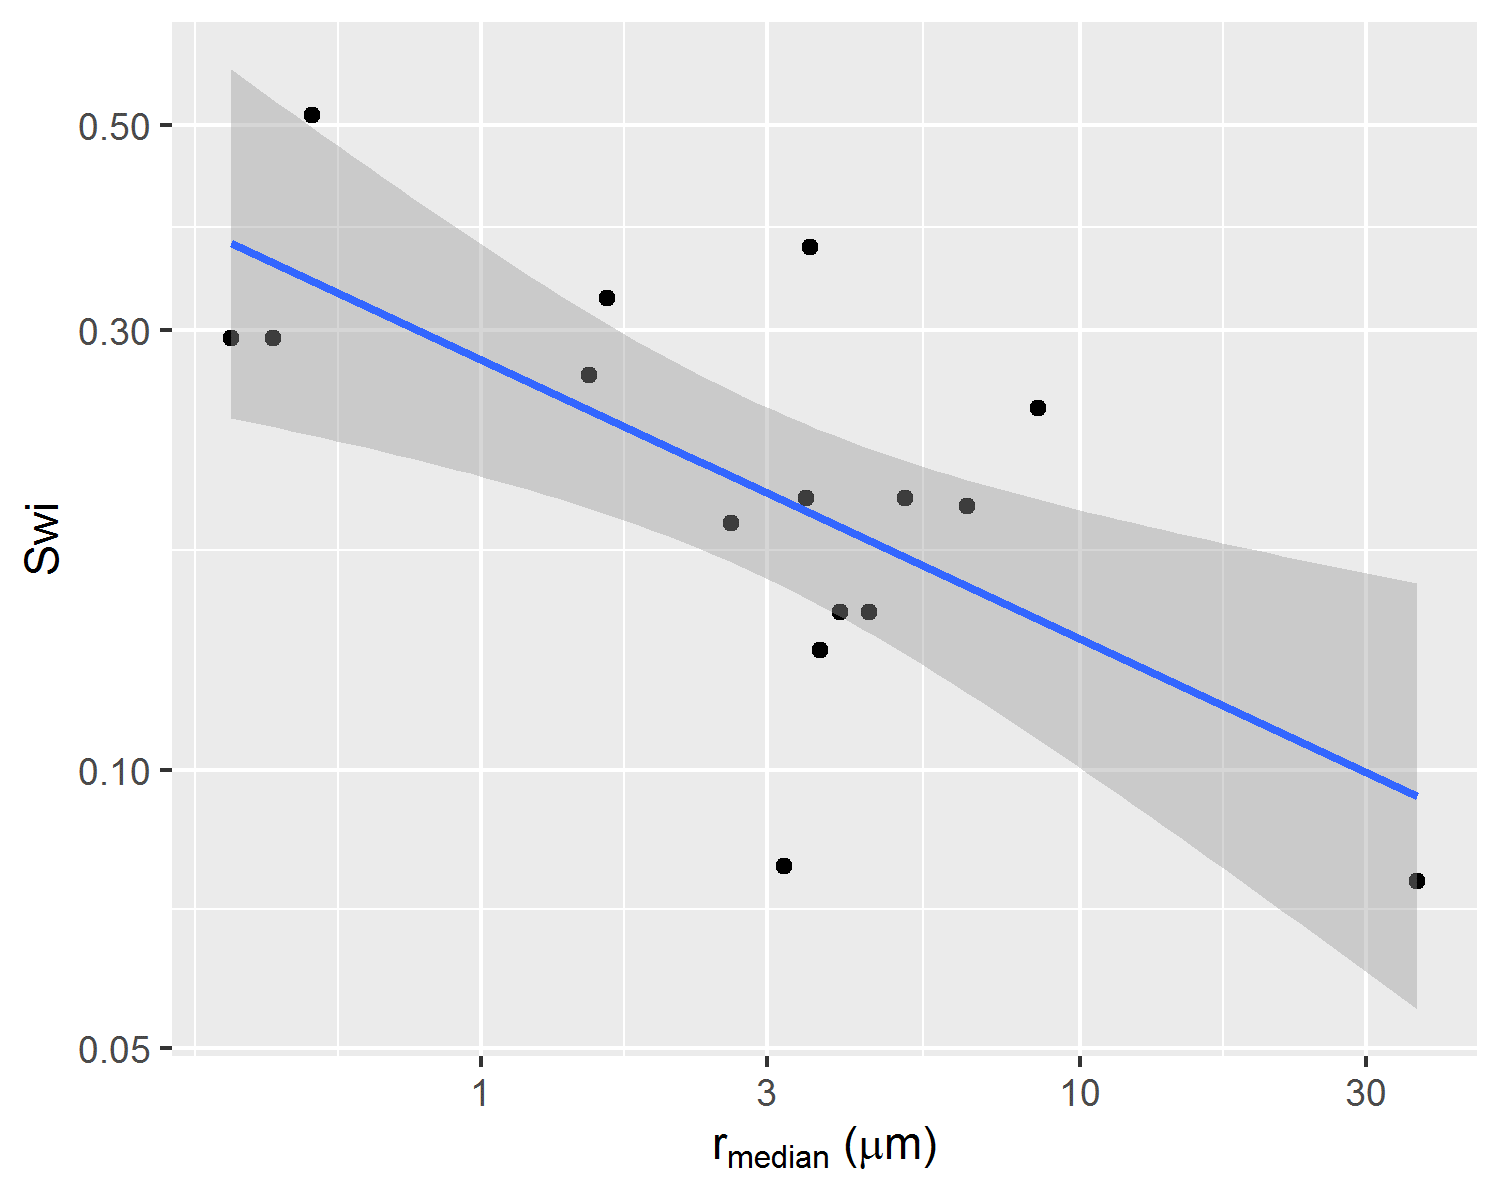
\includegraphics[width=0.45\linewidth]{figure/2-12b-correlations-pchg} 
  
  }
  
  \caption{Correlations between parameters alpha, Swi and median pore throat radius of correspondent rock fragment p(log r) distribution.}\label{fig:pcc-correlations2}
  \end{figure}
  \par
  
  Given \(x\) a vector of input parameters \{\(k_{abs}\), \(r_{35}\), \(iqr\)\} and y a vector of output parameters \{\(S_{wi}\), \(\alpha\), \(\beta\), \(P_e\)\}, and considering a multivariate gaussian distribution described by equation \eqref{eq:normal-eq}, the conditional distribution of the output parameters given known input parameters \(p(y|x)\) may be described by equations \eqref{eq:posterior-distribution}\eqref{eq:posterior-mean}\eqref{eq:posterior-covariance}. Estimating mean and covariance matrix statistics of the multivariate gaussian distribution \eqref{eq:normal-eq} on the assembled dataset, using maximum likelihood methods (DeGroot and Schervish \protect\hyperlink{ref-DeGroot2012}{2012}), inference and uncertainty evaluation may be performed on desired new input \(x\) values.
  \begin{equation} 
    \begin{pmatrix}
    x \\
    y
    \end{pmatrix} \sim \mathcal{N}\left(\begin{pmatrix}
    \mu_x \\
    \mu_y
    \end{pmatrix},\begin{pmatrix}
    \Sigma_{xx} & \Sigma_{xy} \\
    \Sigma_{yy} & \Sigma_{xy}
    \end{pmatrix}\right)
    \label{eq:normal-eq}
  \end{equation}
  \begin{equation} 
    p(y|x) \sim \mathcal{N}(\mu_{y|x}, \Sigma_{y|x})
    \label{eq:posterior-distribution}
  \end{equation}
  \begin{equation} 
    \mu_{y|x} = \mu_y + (\Sigma_{xx}^{-1}\Sigma_{yx})^t(x-\mu_x)
    \label{eq:posterior-mean}
  \end{equation}
  \begin{equation} 
    \Sigma_{y|x} = \Sigma_{yy} - \Sigma_{xy}^{t}\Sigma_{xx}^{-1}\Sigma_{yx}
    \label{eq:posterior-covariance}
  \end{equation}
  Given new \(x=\{k_{abs}, r_{35}, iqr\}\) values, the expected capillary pressure curve parameters \(E[y|x]\) may be obtained by the conditional mean \(\mu_{y|x}\). Uncertainty evaluation of this prediction may be executed using samples of the conditional distribution \(p(y|x)\). Figure \ref{fig:pcc-posterior-sample} displays examples of experimental capillary pressure curves and predictions of these curves using as input associated \(\{k_{abs}, r_{35}, iqr\}\) values. Samples from the conditional distribution \(p(y|x)\) are shown as grey lines and illustrate prediction uncertainty.
  \begin{figure}
  
  {\centering 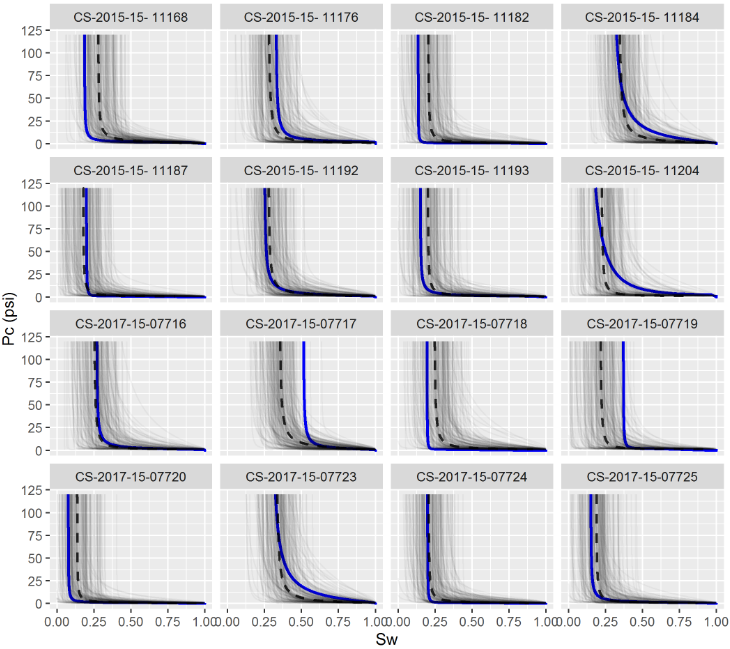
\includegraphics[width=0.9\linewidth]{figure/4-3-pcc-posterior-sample} 
  
  }
  
  \caption{Visual comparison of experimental capillary pressure curves (blue lines), samples from the conditional distribution (grey lines) and average predicted curves (dashed black lines).}\label{fig:pcc-posterior-sample}
  \end{figure}
  \par
  
  On Figure \ref{fig:pcc-posterior-correlations}, a comparison between experimental and predicted capillary pressure curve parameters is shown. Due to inherent noise associated with heterogeneous reservoir rocks and, as also observed in Figure \ref{fig:pcc-posterior-sample}, there is significant dispersion of experimental and predicted parameters values. Both in Figures \ref{fig:pcc-posterior-correlations} and \ref{fig:pcc-posterior-tendency}, it is possible to visualize that capillary curve parameter predictions follow linear tendencies with absolute permeability. This property of linear model predictions is desirable, as it follows the expected physical behavior of reservoir rocks.
  \begin{figure}
  
  {\centering 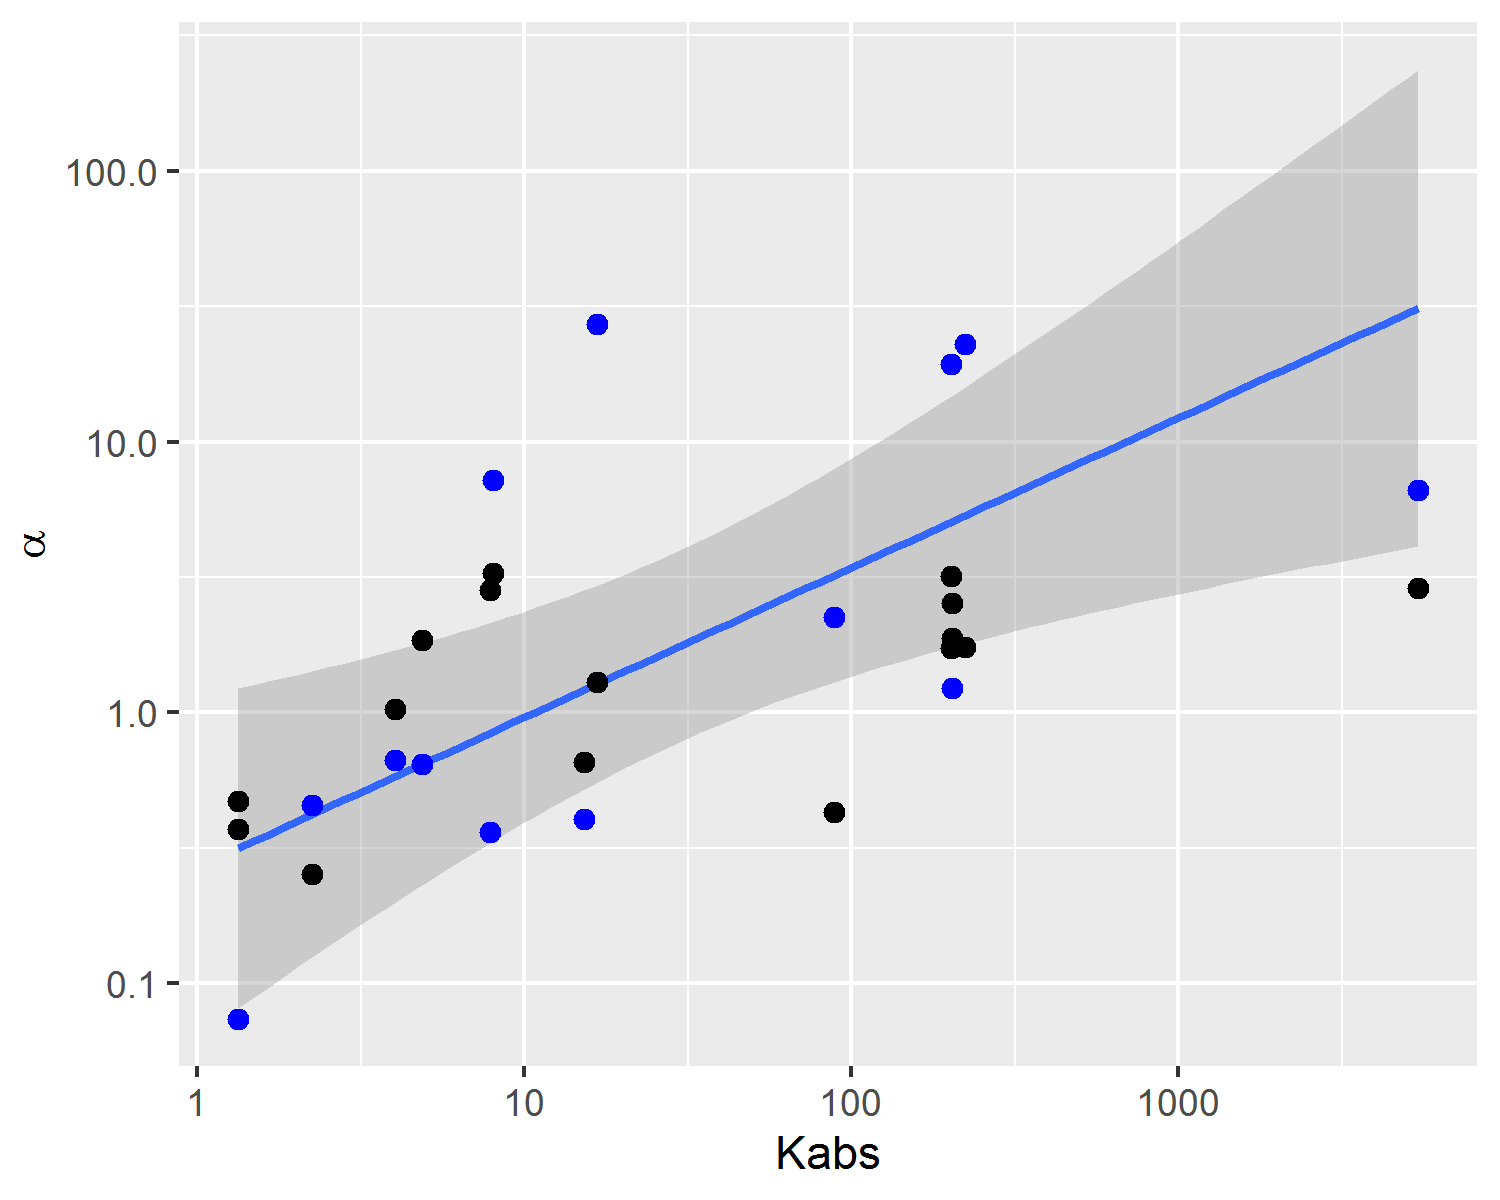
\includegraphics[width=0.45\linewidth]{figure/4-4-pcc-correlation-a} 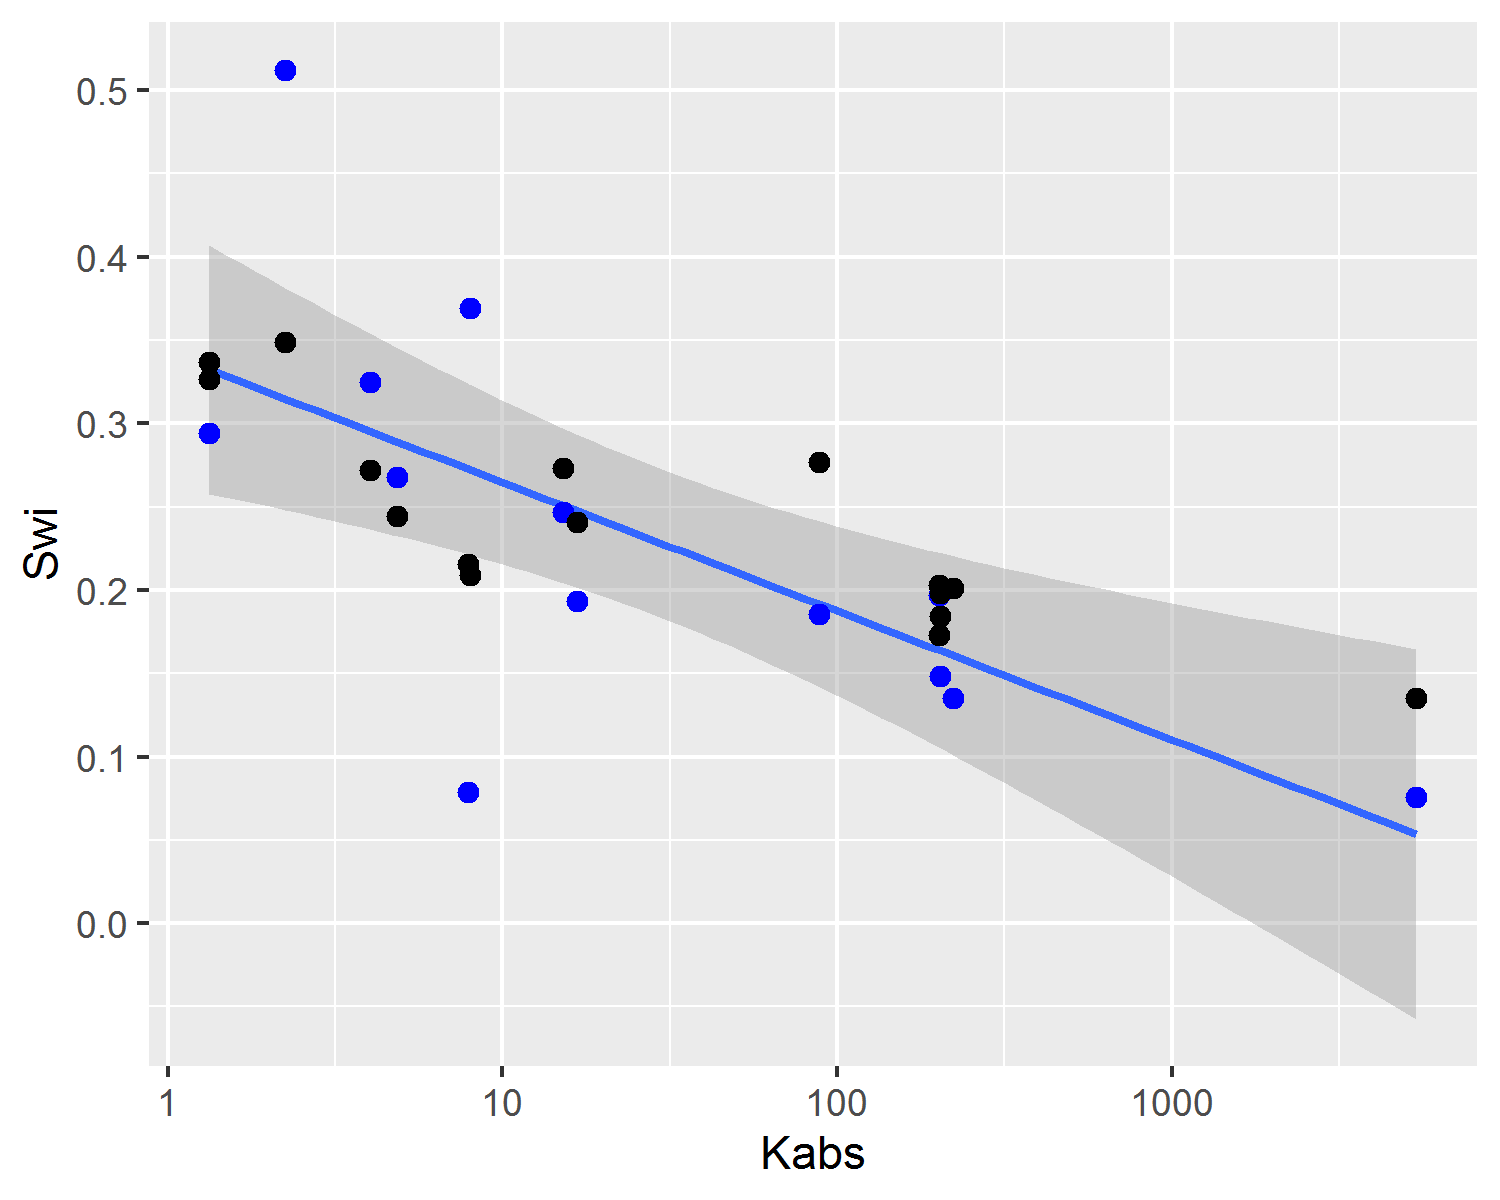
\includegraphics[width=0.45\linewidth]{figure/4-4-pcc-correlation-b} 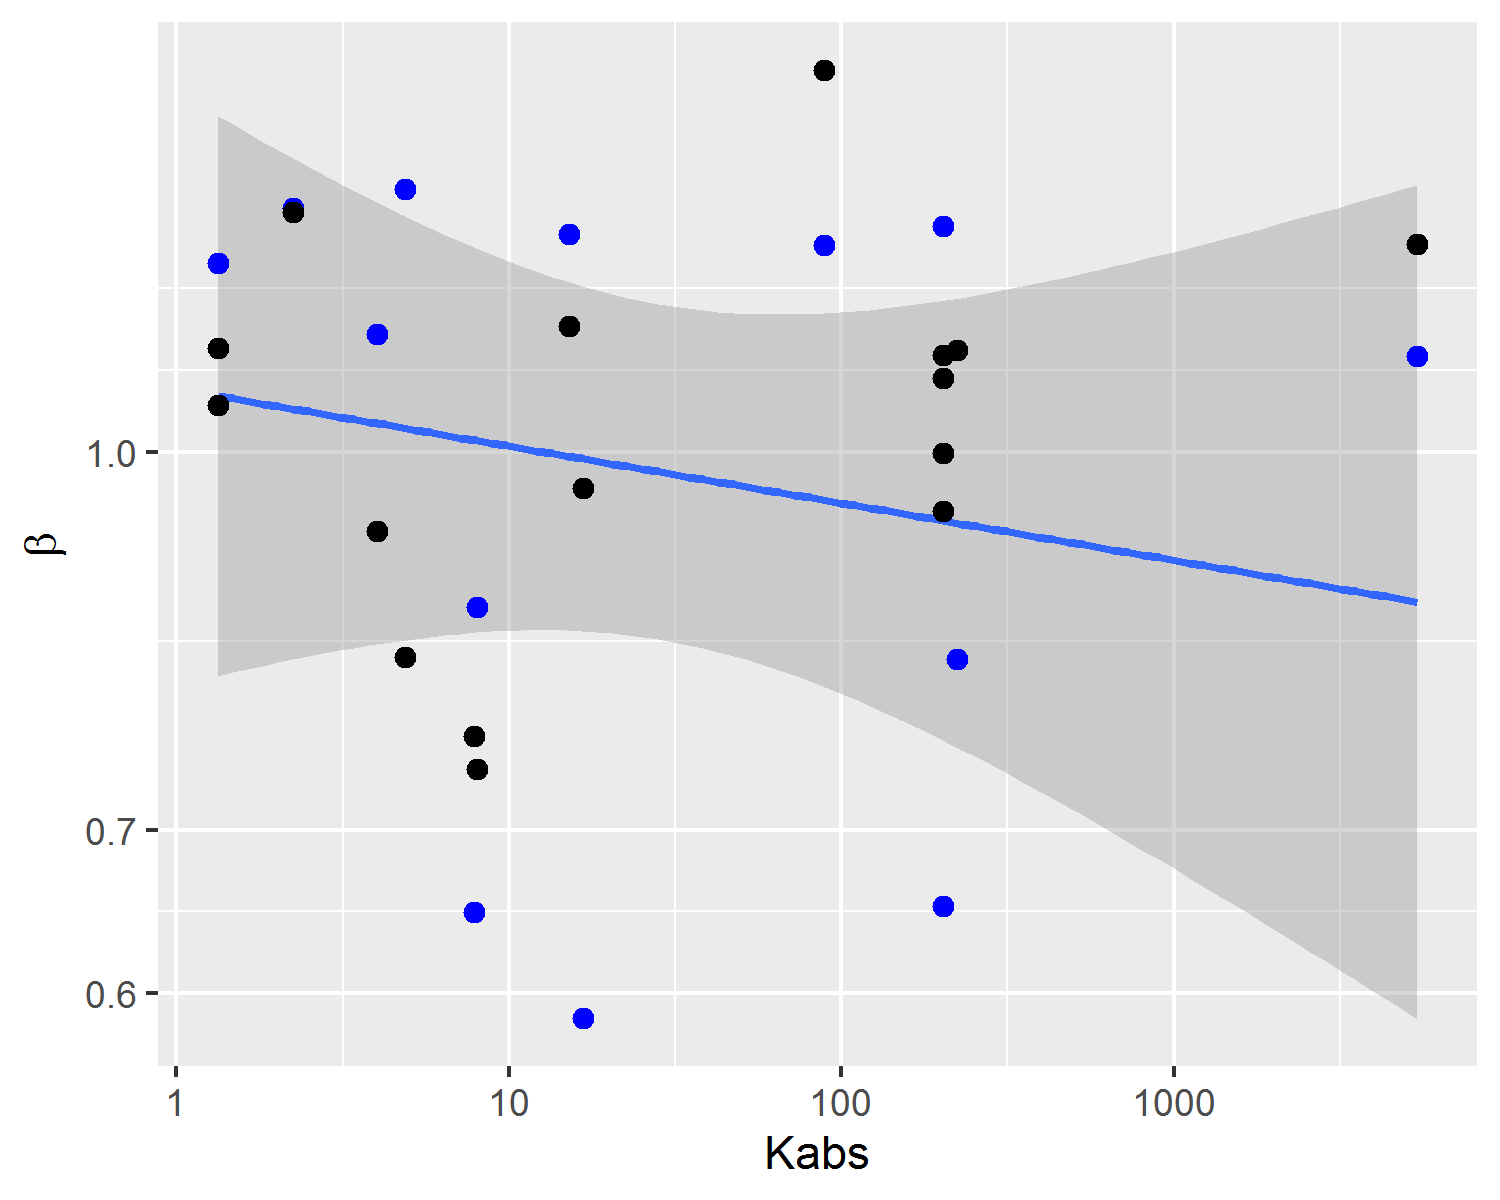
\includegraphics[width=0.45\linewidth]{figure/4-4-pcc-correlation-c} 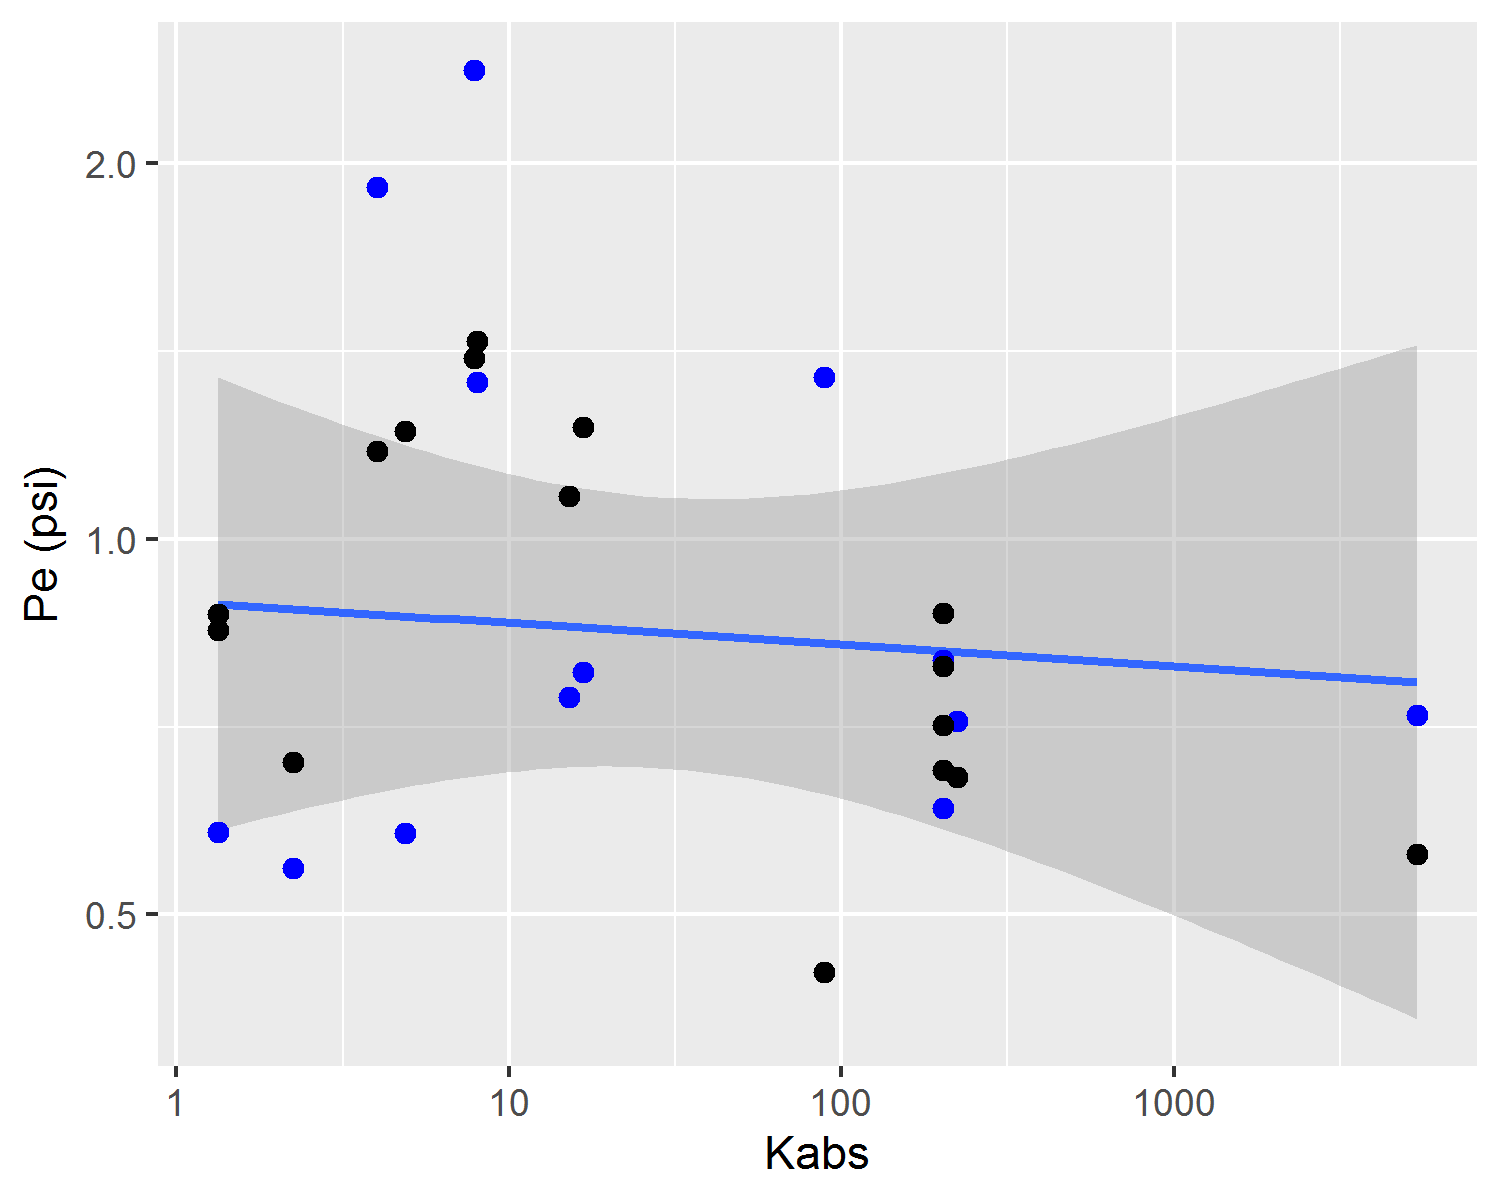
\includegraphics[width=0.45\linewidth]{figure/4-4-pcc-correlation-d} 
  
  }
  
  \caption{Experimental capillary pressure curve parameters (blue dots and line tendency) and predicted parameters estimated using the posterior mean (black dots).}\label{fig:pcc-posterior-correlations}
  \end{figure}
  \begin{figure}
  
  {\centering 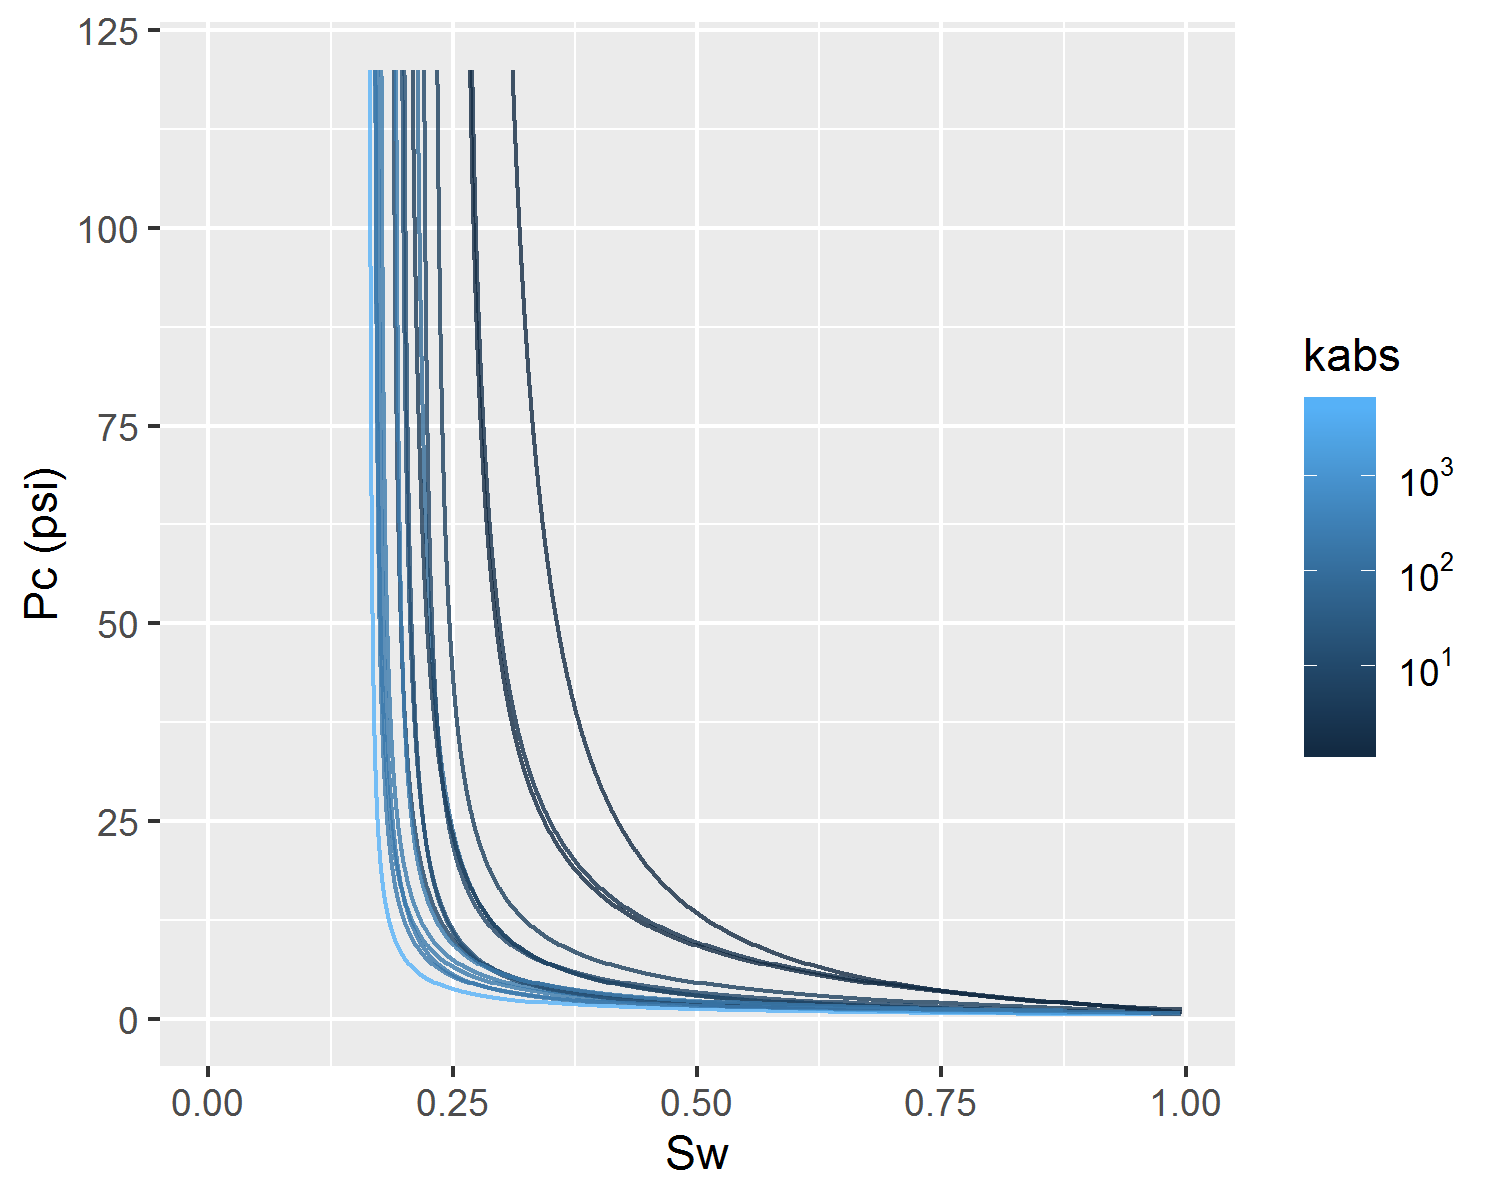
\includegraphics[width=0.7\linewidth]{figure/4-5-pcc-posterior-tendency} 
  
  }
  
  \caption{Behaviour of predicted capillary pressure curves with absolute permeability.}\label{fig:pcc-posterior-tendency}
  \end{figure}
  \hypertarget{hierarchical-linear-regression-1}{%
  \section{Hierarchical Linear Regression}\label{hierarchical-linear-regression-1}}
  
  In a reservoir model, the prediction of petrophysical properties on simulation cells distant from wells with available sampled cores is commonly performed using linear regression methods (Peters \protect\hyperlink{ref-Peters2012}{2012}). To account for sampling bias, special core analysis properties such as relative permeability and capillary pressure are commonly scaled according to reservoir wide available information, such as absolute permeability, porosity and geological facies models. For relative permeability, this procedure is commonly performed using simple linear regression (Gelman et al. \protect\hyperlink{ref-Gelman2014}{2014}) of relative permeability parameters as a function of absolute permeability.
  
  On this work, simple linear and hierarchical linear regression models were evaluated in a dataset containing 226 unsteady-state water-oil relative permeability curves from several Brazilian reservoirs. Parameters for each of the 226 curves were fitted using maximum likelihood estimation (Migon, Gamerman, and Louzada \protect\hyperlink{ref-Migon2015}{2015}) and the LET parameterization \eqref{eq:swd2}\eqref{eq:kro-let2}\eqref{eq:krw-let2} proposed in (Lomeland, Ebeltoft, and Thomas \protect\hyperlink{ref-Lomeland2005}{2005}).
  \begin{equation} 
    S_{wD} = \frac{S_w - S_{wi}}{1 - S_{wi} - S_{or}} 
    \label{eq:swd2}
  \end{equation}
  \begin{equation} 
    k_{ro}(S_w) = k_{ro@S_{wi}}\frac{(1-S_{wD})^{L_o}}{(1-S_{wD})^{L_o} + E_o(S_{wD})^{T_o}}
    \label{eq:kro-let2}
  \end{equation}
  \begin{equation} 
    k_{rw}(S_w) = k_{rw@S_{or}}\frac{(S_{wD})^{L_w}}{(S_{wD})^{L_w} + E_w(1-S_{wD})^{T_w}}
    \label{eq:krw-let2}
  \end{equation}
  Categorical variables, such as field, reservoir or geological facies, may be used to group petrophysical models. A model that does not distinguish between groups, using constant intercept and slope parameters for all categories according to equation \eqref{eq:simple-linear}, may be referred to as a non-pooled model (Gelman et al. \protect\hyperlink{ref-Gelman2014}{2014}). Figure \ref{fig:non-pooled} displays a simple linear non-pooled regression model of irreducible water saturation \(S_{wi}\) as the predicted \(y\) variable and the logarithm of absolute permeability \(\log{k_{abs}}\) as the observed \(x\) variable. On equation \eqref{eq:simple-linear}, \(n\) represents the total number of data samples, indexed by the letter \(i\), and \(\alpha\), \(\beta\) and \(\sigma_y^2\) represent the intercept, slope and variance linear model parameters.
  \begin{equation} 
    y_i \sim \mathcal{N}(\alpha + \beta x, \sigma_y^2),\quad \text{for}\; i=1,...,n
    \label{eq:simple-linear}
  \end{equation}
  \begin{figure}
  
  {\centering 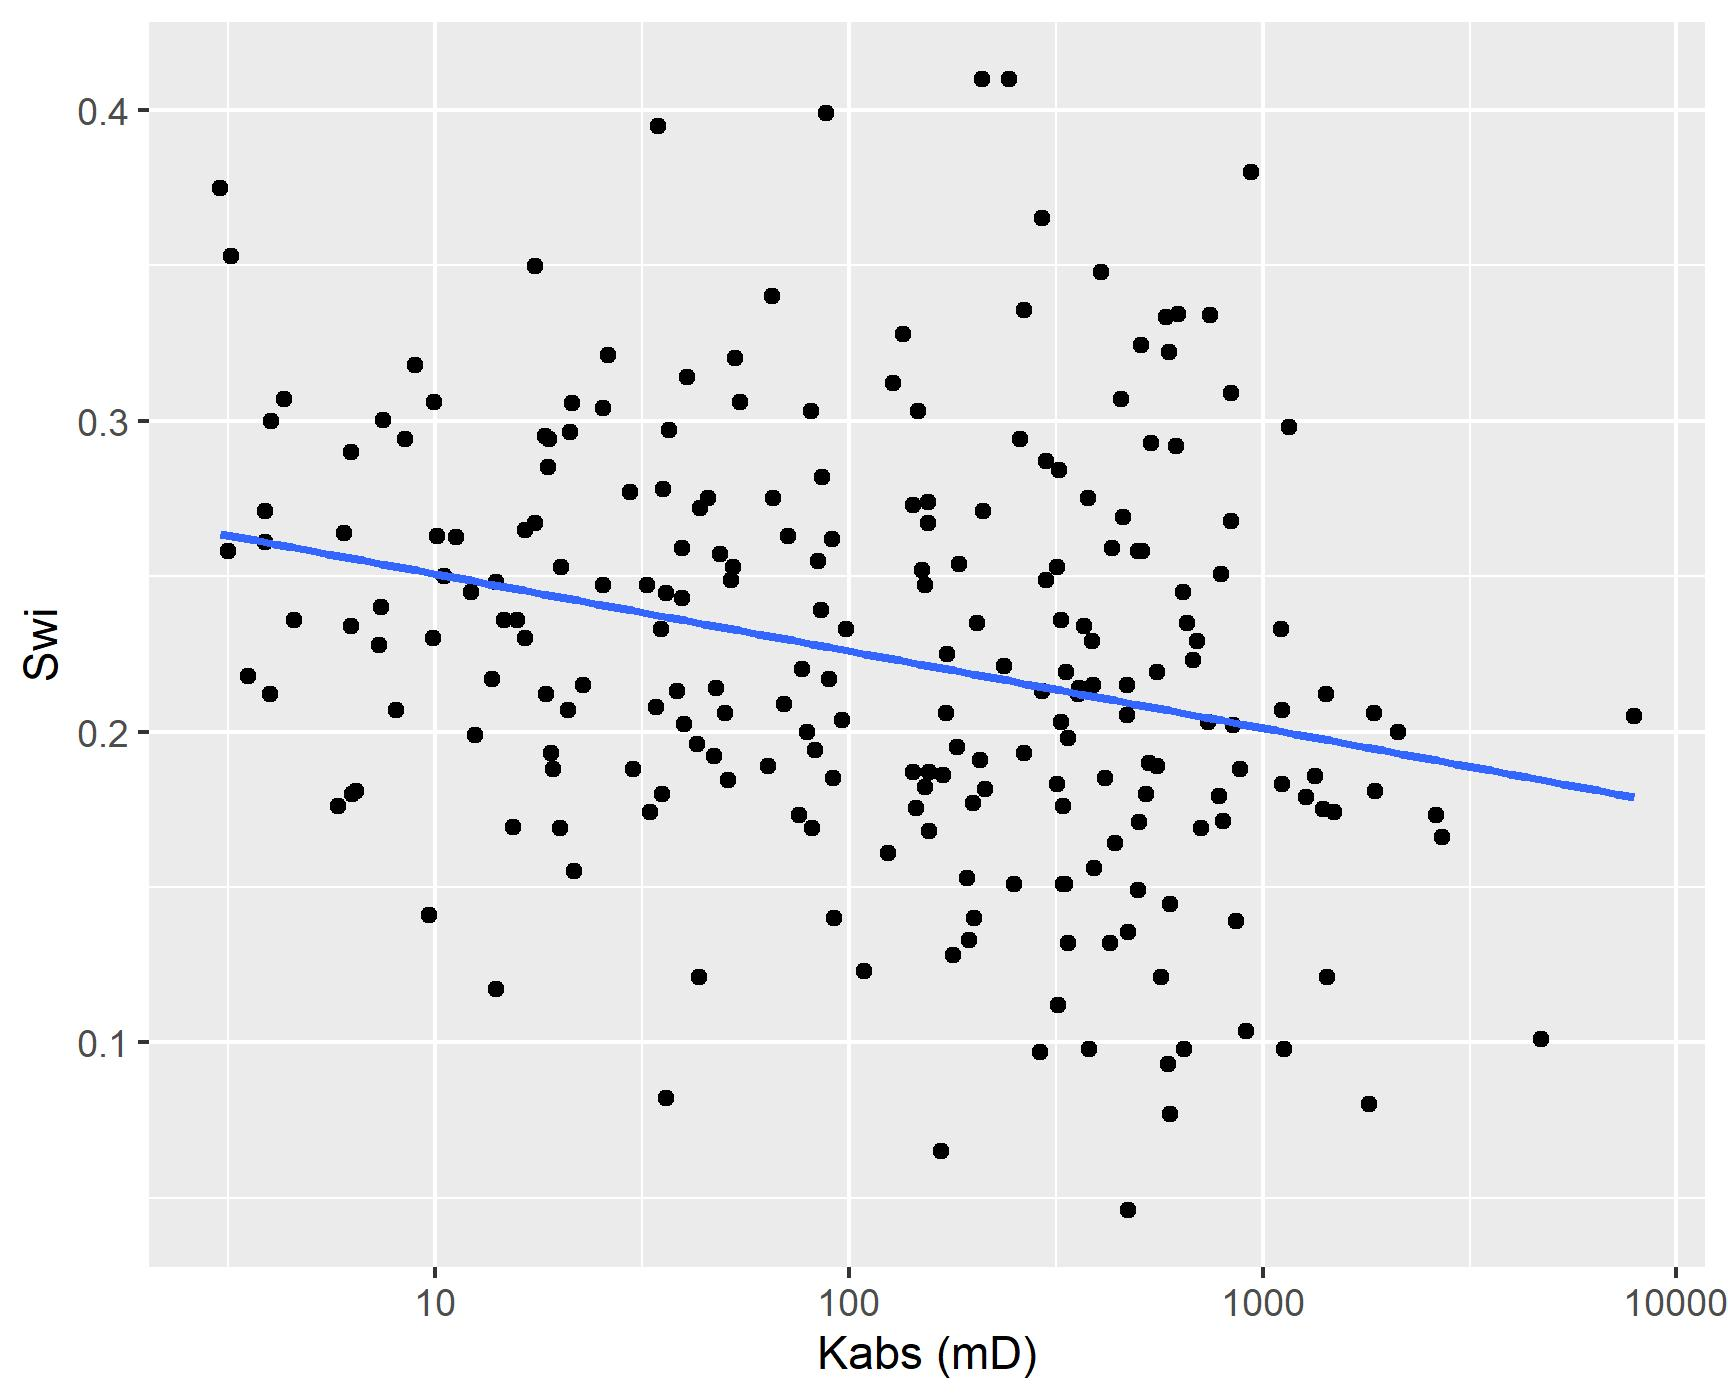
\includegraphics[width=0.9\linewidth]{figure/4-6-simple-regression} 
  
  }
  
  \caption{Non-pooled simple linear regression.}\label{fig:non-pooled}
  \end{figure}
  Usually, though, separate linear regression models are fitted to each category of interest, in models that may be referred to as completely pooled. For each category \(j\), independent \(\alpha_j\), \(\beta_j\) and \(\sigma_{y^j}^2\) parameters are estimated, as described in equation \eqref{eq:simple-linear-full}.
  \begin{equation} 
    y_i^j \sim \mathcal{N}(\alpha_j + \beta_j x_i^j, \sigma_{y^j}^2),\quad \text{for}\; i=1,...,n; \quad \text{for} \; i=1,...,J
    \label{eq:simple-linear-full}
  \end{equation}
  Figure \ref{fig:completely-pooled} displays a simple linear completely pooled regression model of irreducible water saturation \(S_{wi}\) and the logarithm of absolute permeability \(\log{k_{abs}}\), grouped by reservoir. In completely pooled regression models, each linear regression model is independent of each other, with varying degrees of uncertainty on each model parameters \(\alpha_j\), \(\beta_j\) and \(\sigma_{y^j}^2\). Categories with larger number of samples and smaller heterogeneities, usually display smaller uncertainties on model parameters.
  \begin{figure}
  
  {\centering 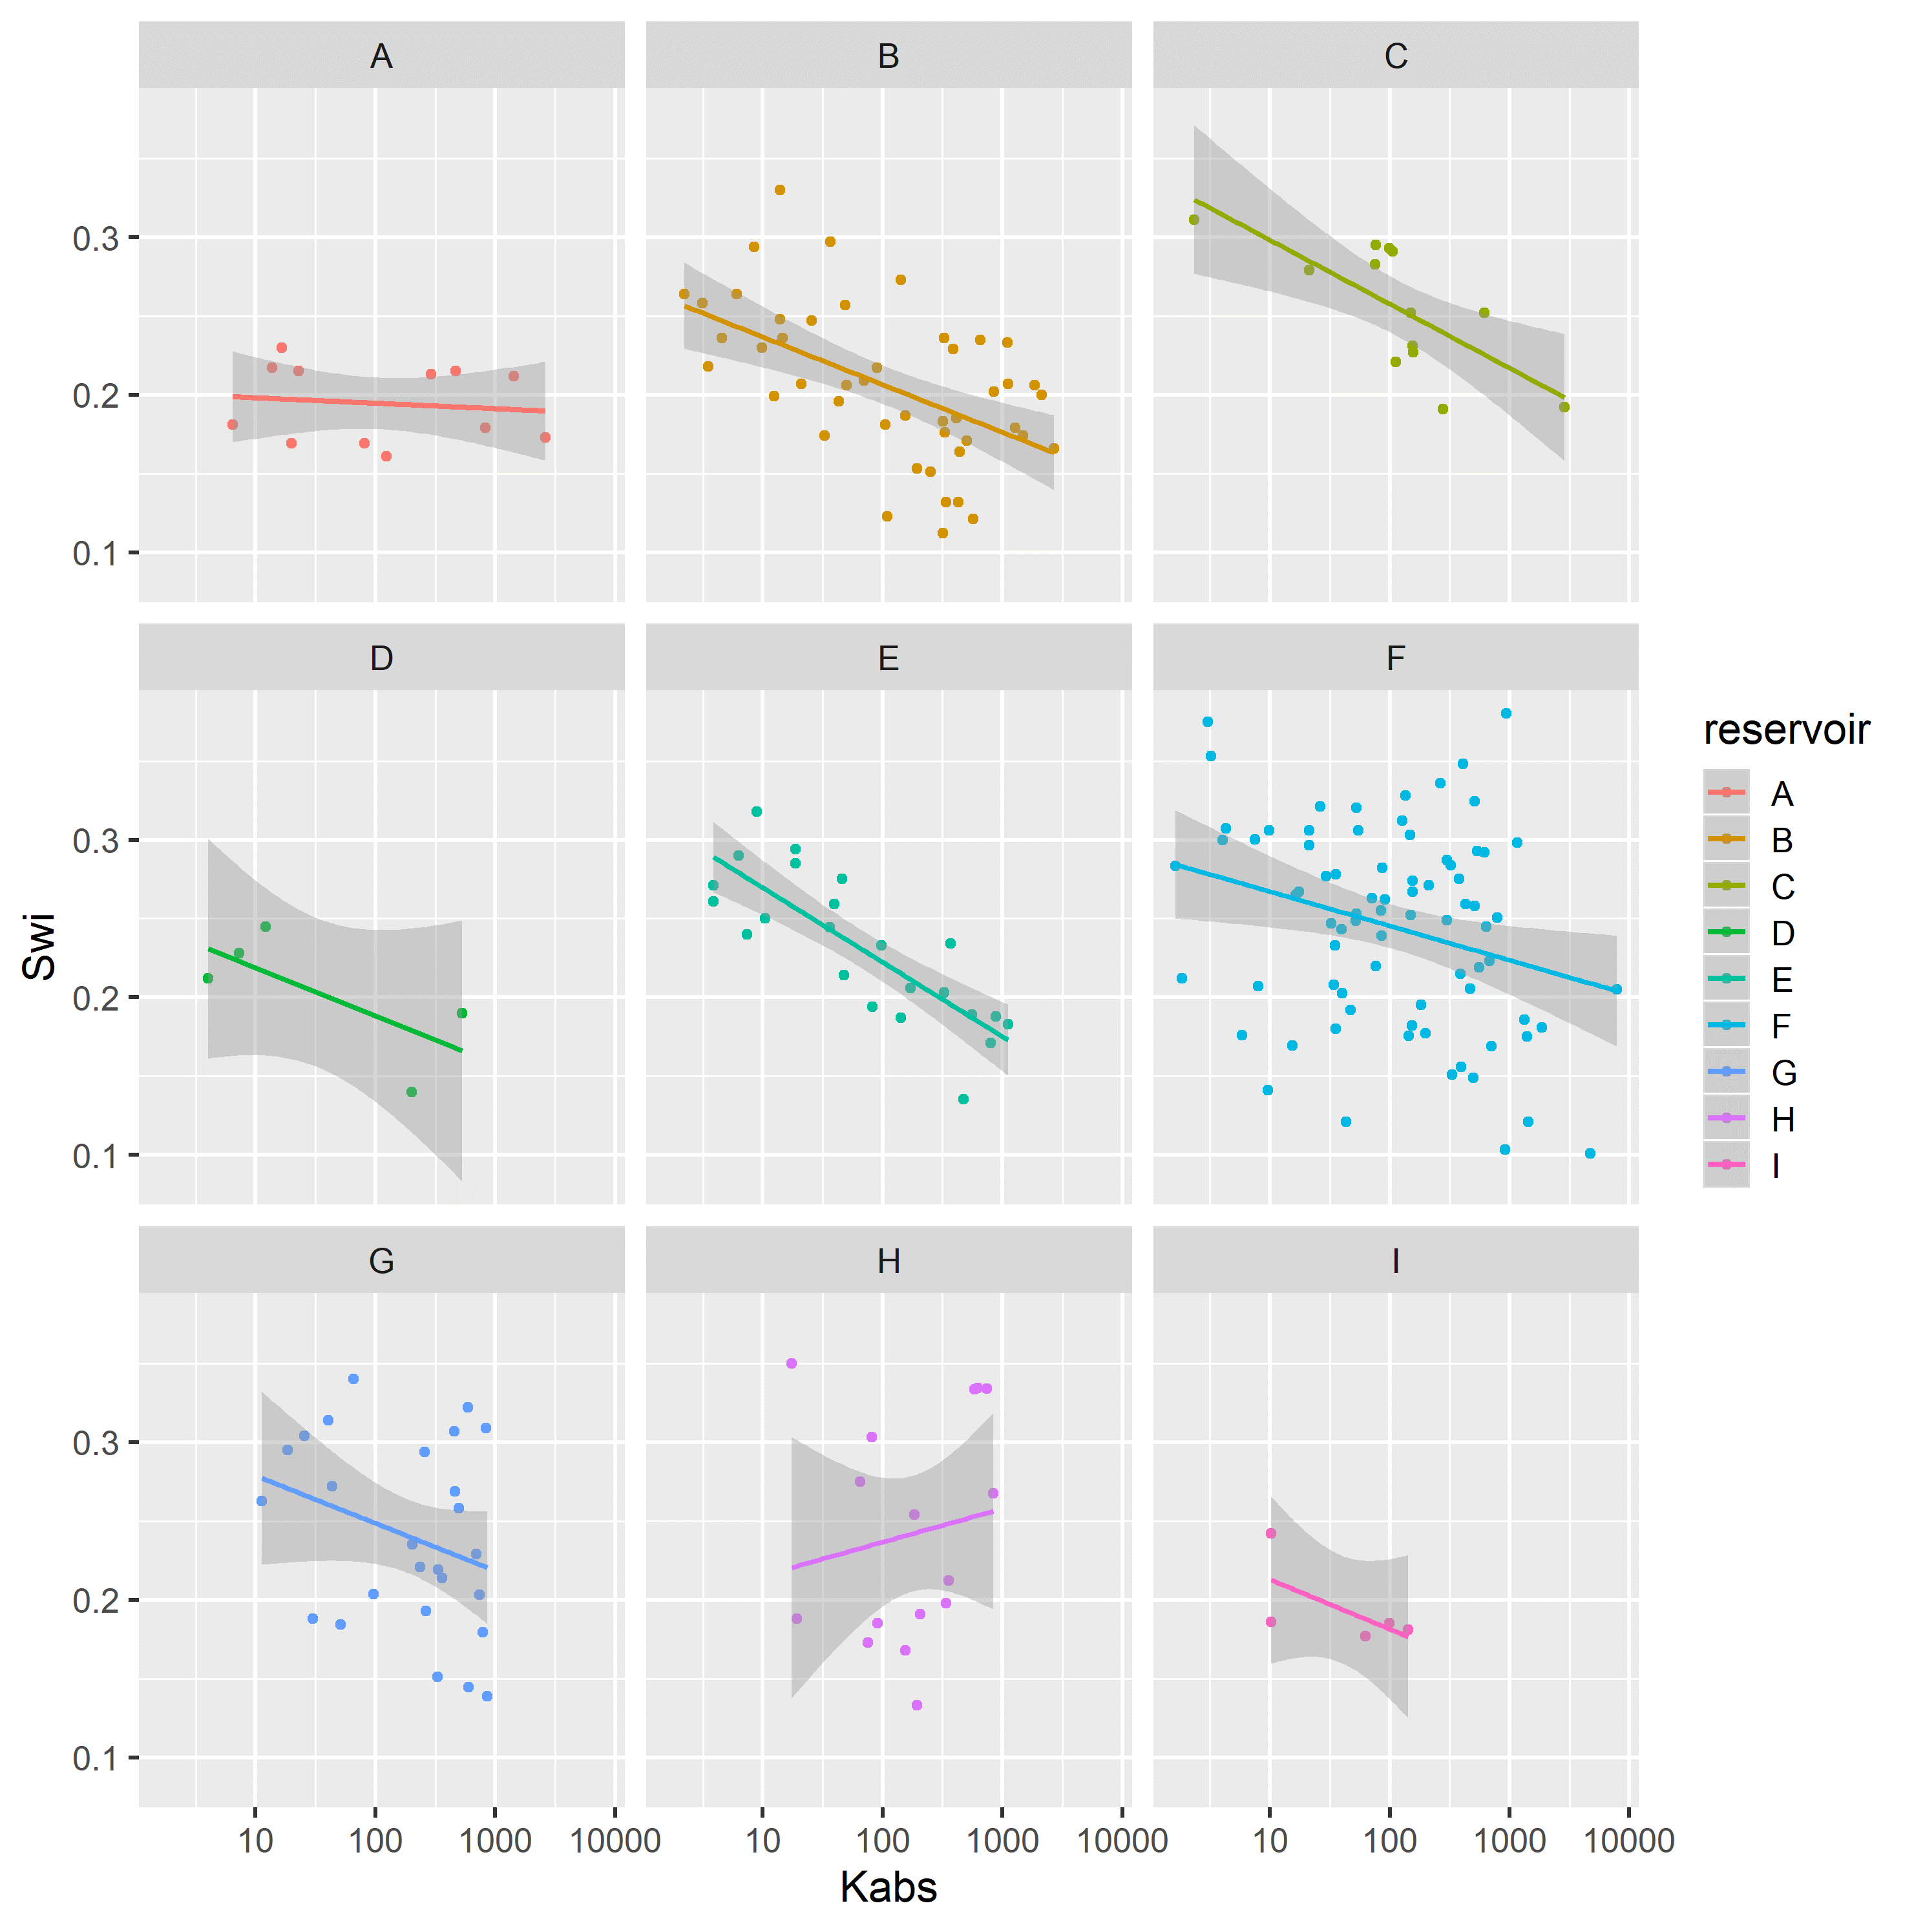
\includegraphics[width=0.9\linewidth]{figure/4-7-completely-pooled} 
  
  }
  
  \caption{Completely pooled simple linear regression models, grouped by reservoir.}\label{fig:completely-pooled}
  \end{figure}
  \par
  
  Hierarchical or partially pooled linear regression models introduce information sharing and coupling between model parameters of different categories, modeling intercept and/or slope parameters as sampled from a latent parent distribution.
  
  Varying intercept models, assume that the intercept of each category \(\alpha_j\) is sampled from a common latent gaussian distribution \eqref{eq:varying-intercepts-b}. This information sharing, has a regularizing effect of shrinking the partially pooled parameters towards a common mean \(\mu_\alpha\).
  \begin{equation} 
    y_i^j \sim \mathcal{N}(\alpha_j + \beta_j x_i^j, \sigma_{y^j}^2),\quad \text{for}\; i=1,...,n; \quad \text{for} \; j=1,...,J
    \label{eq:varying-intercepts-a}
  \end{equation}
  \begin{equation} 
    \alpha_j \sim \mathcal{N}(\mu_\alpha, \sigma_\alpha^2), \quad \text{for} \; j=1,...,J
    \label{eq:varying-intercepts-b}
  \end{equation}
  Varying slope models, assume that the slope of each category \(\beta_j\) is sampled from a common latent gaussian distribution \eqref{eq:varying-slopes-b}, with the same regularizing effect of shrinking the partially pooled parameters towards a common mean \(\mu_\beta\).
  \begin{equation} 
    y_i^j \sim \mathcal{N}(\alpha_j + \beta_j x_i^j, \sigma_{y^j}^2),\quad \text{for}\; i=1,...,n; \quad \text{for} \; j=1,...,J
    \label{eq:varying-slopes-a}
  \end{equation}
  \begin{equation} 
    \beta_j \sim \mathcal{N}(\mu_\beta, \sigma_\beta^2), \quad \text{for} \; j=1,...,J
    \label{eq:varying-slopes-b}
  \end{equation}
  Varying intercept and slope models, assume that both the intercept and slope of each category \(\alpha_j\) and \(\beta_j\) are sampled from a common latent multivariate gaussian distribution \eqref{eq:varying-intercepts-slopes-b}.
  \begin{equation} 
    y_i^j \sim \mathcal{N}(\alpha_j + \beta_j x_i^j, \sigma_{y^j}^2),\quad \text{for}\; i=1,...,n; \quad \text{for} \; j=1,...,J
    \label{eq:varying-intercepts-slopes-a}
  \end{equation}
  \begin{equation} 
    \begin{pmatrix}
    \alpha_j \\
    \beta_j
    \end{pmatrix} \sim \mathcal{N}\left(\begin{pmatrix}
    \mu_\alpha \\
    \mu_\beta
    \end{pmatrix},\begin{pmatrix}
    \sigma_\alpha^2 & \rho \sigma_\alpha \sigma_\beta \\
    \rho \sigma_\alpha \sigma_\beta & \sigma_\beta^2
    \end{pmatrix}\right),\quad \text \quad \text{for} \; j=1,...,J
    \label{eq:varying-intercepts-slopes-b}
  \end{equation}
  For the dataset of 226 unsteady-state water-oil relative permeability curve LET parameters, hierarchical varying slope models of relative permeability endpoint parameters \(S_{wi}\), \(S_{or}\), \(k_{ro}@S_{wi}\) and \(k_{rw}@S_{or}\), and logarithm of absolute permeability \(\log{k_{abs}}\) were fit and compared to completely pooled simple linear regression models, grouped by reservoir.
  
  Both hierarchical and simple linear regression model parameters were inferred using bayesian Hamiltonian Markov-Chain Monte-Carlo (Hoffman and Gelman \protect\hyperlink{ref-Hoffman2014}{2014}) and the software Stan (Carpenter et al. \protect\hyperlink{ref-Carpenter2017}{2017}). Default weakly informative model parameter priors were utilized, following the recommendations of (Gelman et al. \protect\hyperlink{ref-Gelman2008}{2008}).
  
  Comparison between hierarchical and simple linear regression models were performed using the root mean squared error RMSE, the Watanabe-Akaike Information Criteria (WAIC), the leave-one-out information criteria (LOOIC), and the bayesian R-squared \(R^2\) and adjusted R-squared \(R_{adj}^2\) metrics (Gelman et al. \protect\hyperlink{ref-GelmanGoodrich2019}{2019})(Vehtari, Gelman, and Gabry \protect\hyperlink{ref-Vehtari2017}{2017}). The WAIC and LOOIC information criteria provide a trade-off between goodness-of-fit and model complexity, with lower WAIC and LOOIC values corresponding to lower cross-validation errors.
  
  Hierarchical varying slope and simple linear regression models of irreducible water saturation \(S_{wi}\) and logarithm of absolute permeability \(\log{k_{abs}}\) were evaluated on the assembled dataset.
  
  Table \ref{tab:swi-regression-metrics} displays the obtained regression metrics for each fitted model. Hierarchical linear regression achieved slightly better WAIC, LOOIC and \(R_{adj}^2\) metrics.
  \begin{longtable}[]{@{}ccclll@{}}
  \caption{\label{tab:swi-regression-metrics} \(S_{wi}\) linear regression model metrics.}\tabularnewline
  \toprule
  \begin{minipage}[b]{0.36\columnwidth}\centering
  Regression Model\strut
  \end{minipage} & \begin{minipage}[b]{0.08\columnwidth}\centering
  RMSE\strut
  \end{minipage} & \begin{minipage}[b]{0.11\columnwidth}\centering
  WAIC\strut
  \end{minipage} & \begin{minipage}[b]{0.09\columnwidth}\raggedright
  LOOIC\strut
  \end{minipage} & \begin{minipage}[b]{0.06\columnwidth}\raggedright
  \(R^2\)\strut
  \end{minipage} & \begin{minipage}[b]{0.13\columnwidth}\raggedright
  \(R_{adj}^2\)\strut
  \end{minipage}\tabularnewline
  \midrule
  \endfirsthead
  \toprule
  \begin{minipage}[b]{0.36\columnwidth}\centering
  Regression Model\strut
  \end{minipage} & \begin{minipage}[b]{0.08\columnwidth}\centering
  RMSE\strut
  \end{minipage} & \begin{minipage}[b]{0.11\columnwidth}\centering
  WAIC\strut
  \end{minipage} & \begin{minipage}[b]{0.09\columnwidth}\raggedright
  LOOIC\strut
  \end{minipage} & \begin{minipage}[b]{0.06\columnwidth}\raggedright
  \(R^2\)\strut
  \end{minipage} & \begin{minipage}[b]{0.13\columnwidth}\raggedright
  \(R_{adj}^2\)\strut
  \end{minipage}\tabularnewline
  \midrule
  \endhead
  \begin{minipage}[t]{0.36\columnwidth}\centering
  Simple Linear Regression\strut
  \end{minipage} & \begin{minipage}[t]{0.08\columnwidth}\centering
  0.05\strut
  \end{minipage} & \begin{minipage}[t]{0.11\columnwidth}\centering
  -681.48\strut
  \end{minipage} & \begin{minipage}[t]{0.09\columnwidth}\raggedright
  -680.96\strut
  \end{minipage} & \begin{minipage}[t]{0.06\columnwidth}\raggedright
  0.20\strut
  \end{minipage} & \begin{minipage}[t]{0.13\columnwidth}\raggedright
  0.16\strut
  \end{minipage}\tabularnewline
  \begin{minipage}[t]{0.36\columnwidth}\centering
  Hierarchical Linear Regression\strut
  \end{minipage} & \begin{minipage}[t]{0.08\columnwidth}\centering
  0.05\strut
  \end{minipage} & \begin{minipage}[t]{0.11\columnwidth}\centering
  -684.89\strut
  \end{minipage} & \begin{minipage}[t]{0.09\columnwidth}\raggedright
  -684.66\strut
  \end{minipage} & \begin{minipage}[t]{0.06\columnwidth}\raggedright
  0.24\strut
  \end{minipage} & \begin{minipage}[t]{0.13\columnwidth}\raggedright
  0.17\strut
  \end{minipage}\tabularnewline
  \bottomrule
  \end{longtable}
  Figure \ref{fig:swi-simple-hierarchical} displays simple and hierarchical linear regression \(S_{wi}\) vs \(\log{k_{abs}}\) models, grouped by reservoir. Black dots represent observed samples, light blue lines represent samples from the posterior distribution of intercept and slope parameters, and dark blue lines represent mean intercept and slope parameters, for each reservoir.
  
  Completely pooled, simple linear regression models display larger between-groups slope variations and uncertainty, as shown in Figure \ref{fig:swi-simple-hierarchical-coefs}. Reservoirs with large number of samples, such as reservoir F, display only small changes between hierarchical and simple linear regression model posterior distributions. A stronger regularizing effect is displayed in reservoir H, which contains a small number of samples. Overall behavior consistency of \(S_{wi}\) with respect to \(\log{k_{abs}}\) is increased in the hierarchical partially pooled linear model, as slopes are regressed towards a common mean. As information is shared between different reservoirs, posterior uncertainties are noticeably reduced in the hierarchical linear model.
  \begin{figure}
  
  {\centering 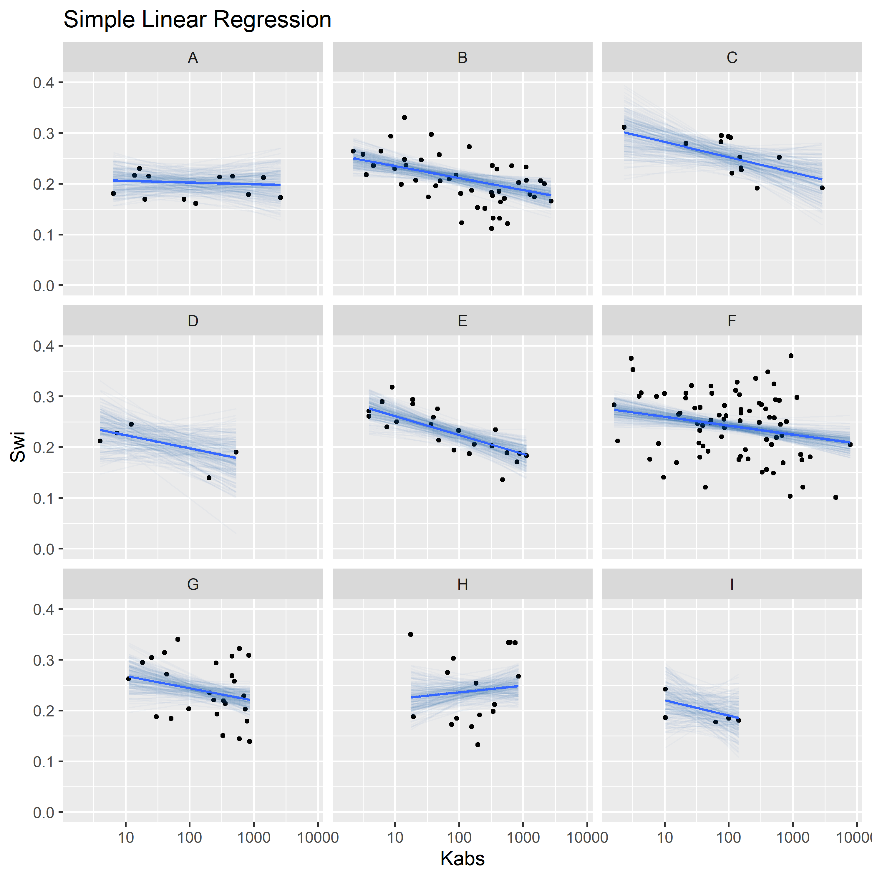
\includegraphics[width=0.75\linewidth]{figure/4-8-swi-simple} 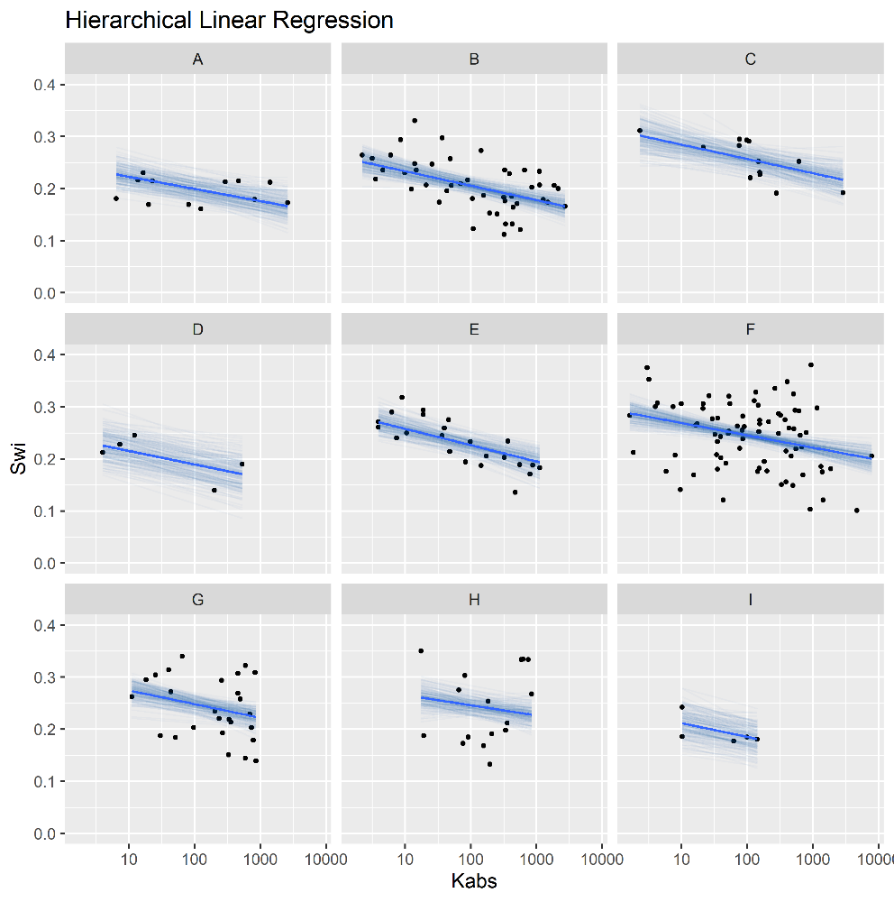
\includegraphics[width=0.75\linewidth]{figure/4-8-swi-hierarchical} 
  
  }
  
  \caption{Simple (top) and Hierarchical (bottom) linear regression models of Swi vs log(kabs), grouped by reservoir.}\label{fig:swi-simple-hierarchical}
  \end{figure}
  \begin{figure}
  
  {\centering 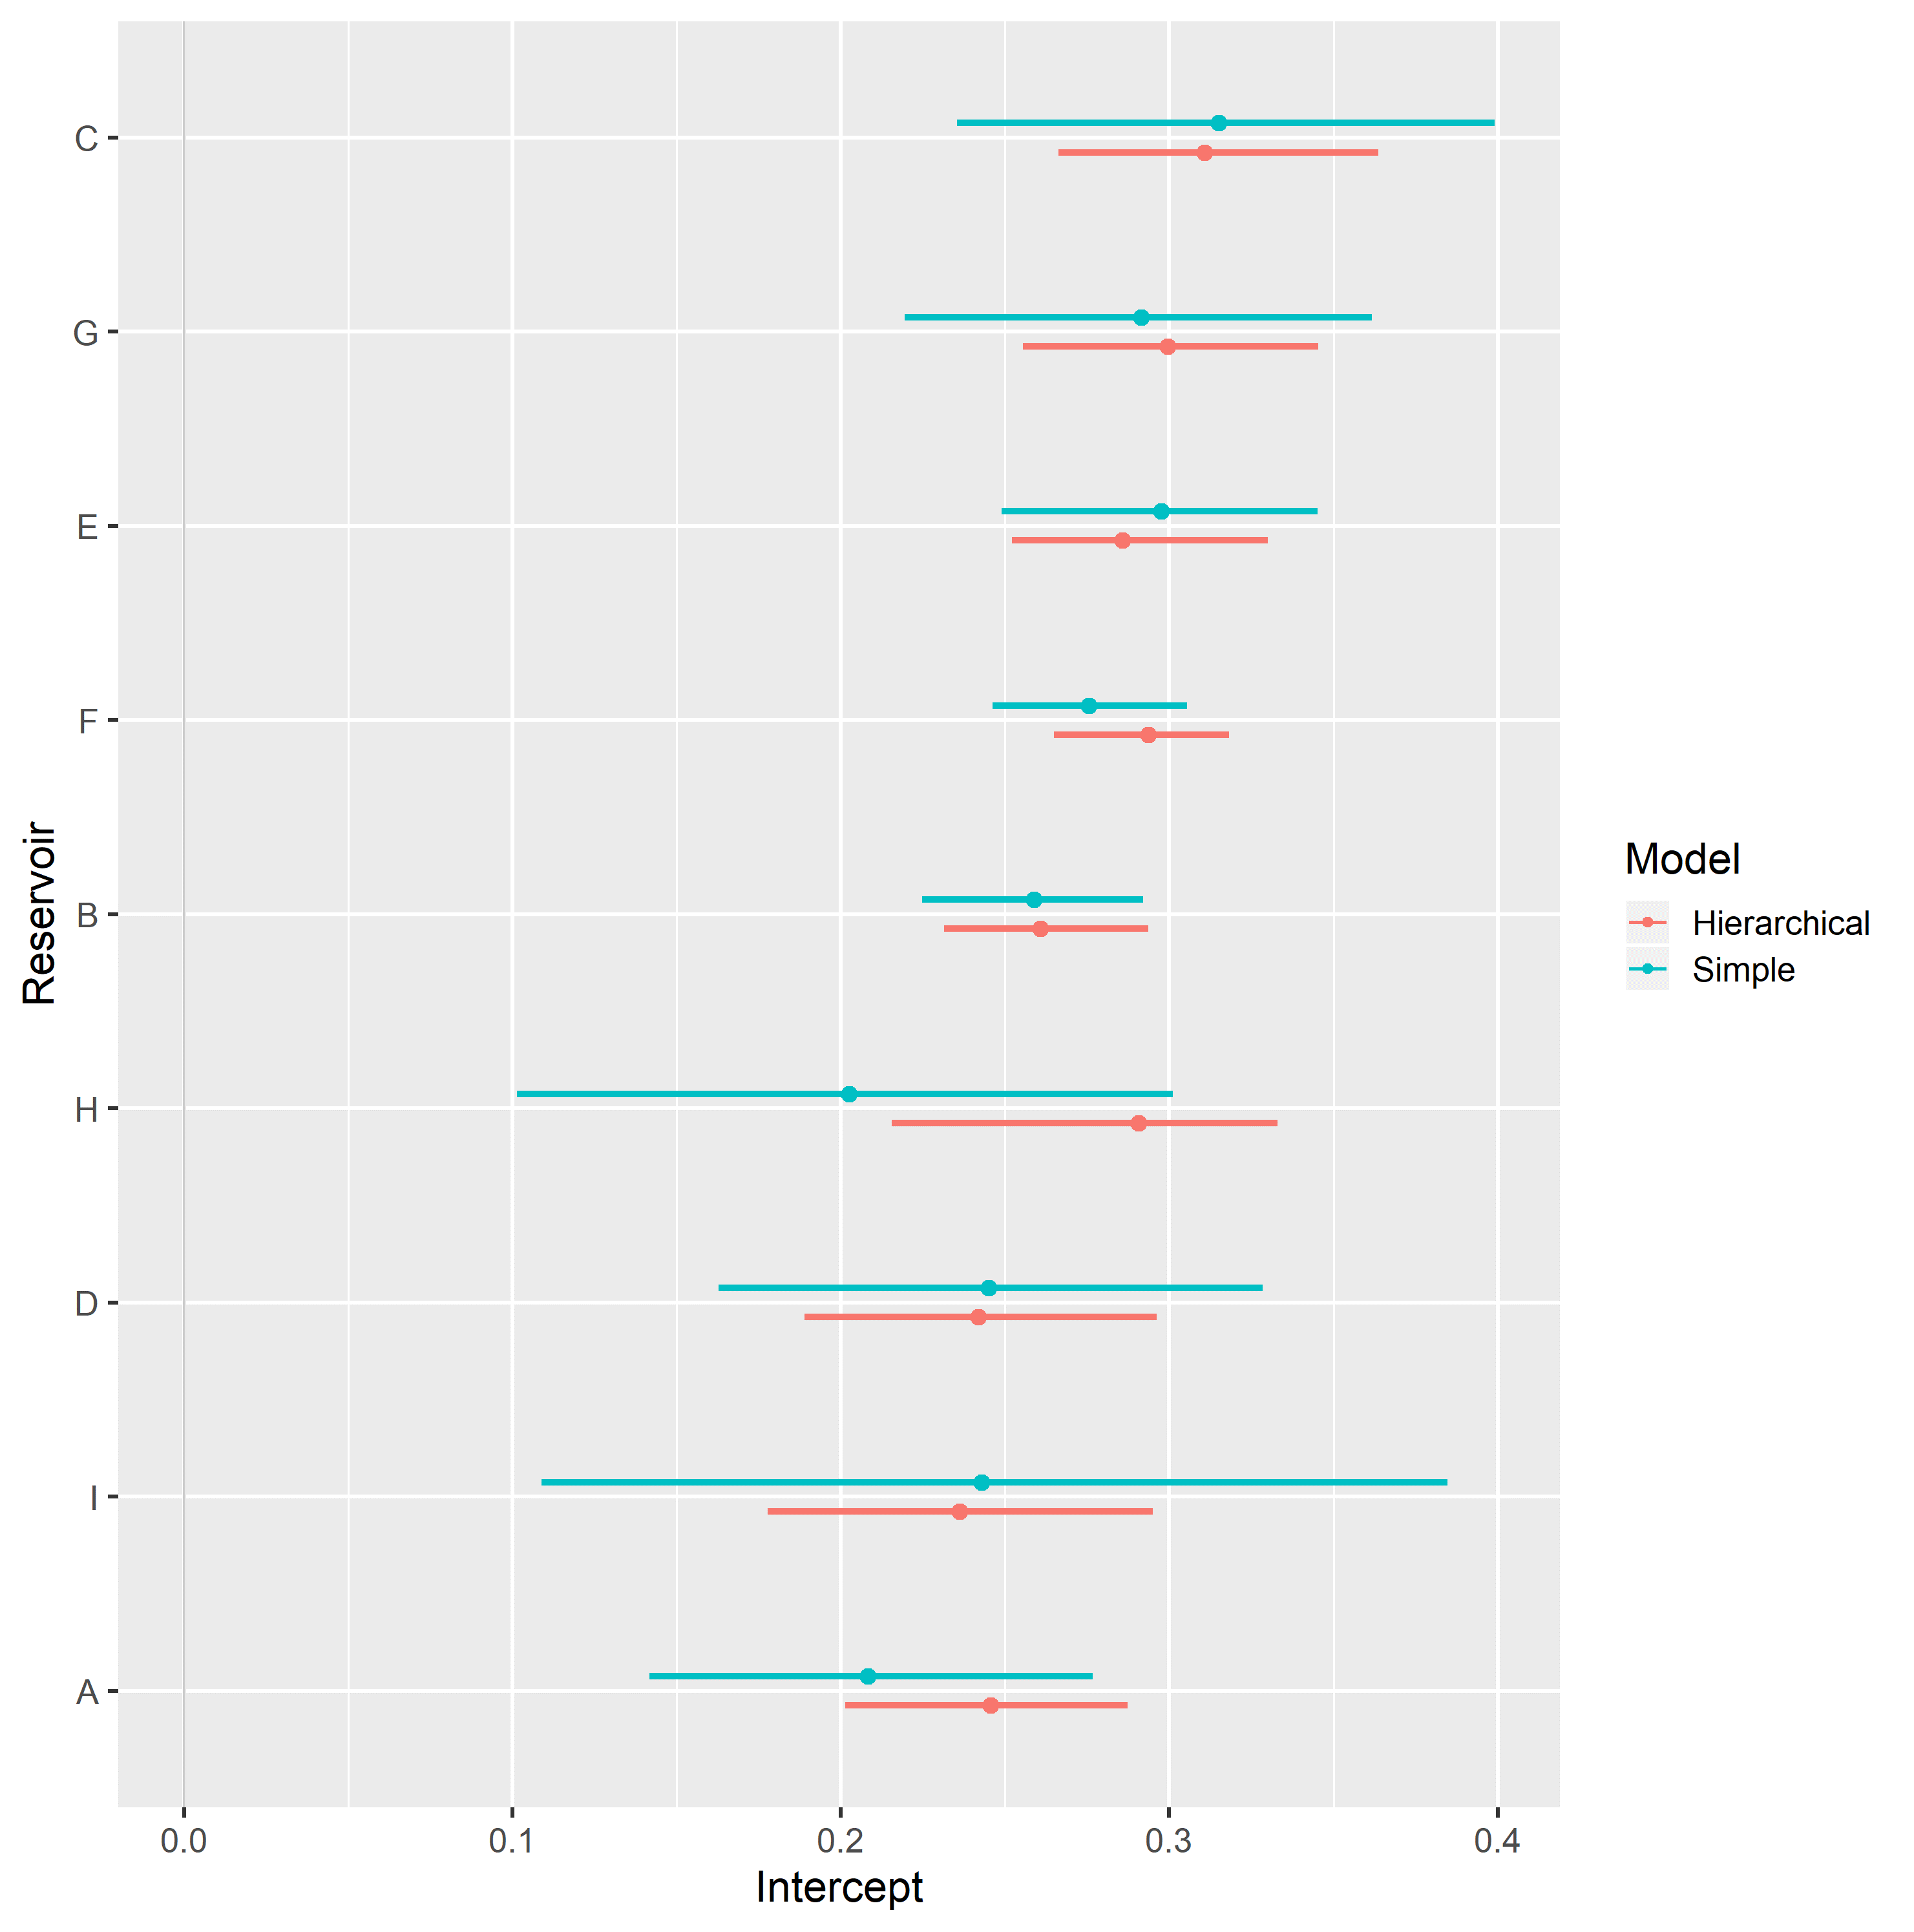
\includegraphics[width=0.75\linewidth]{figure/4-9-swi-coefs-intercept} 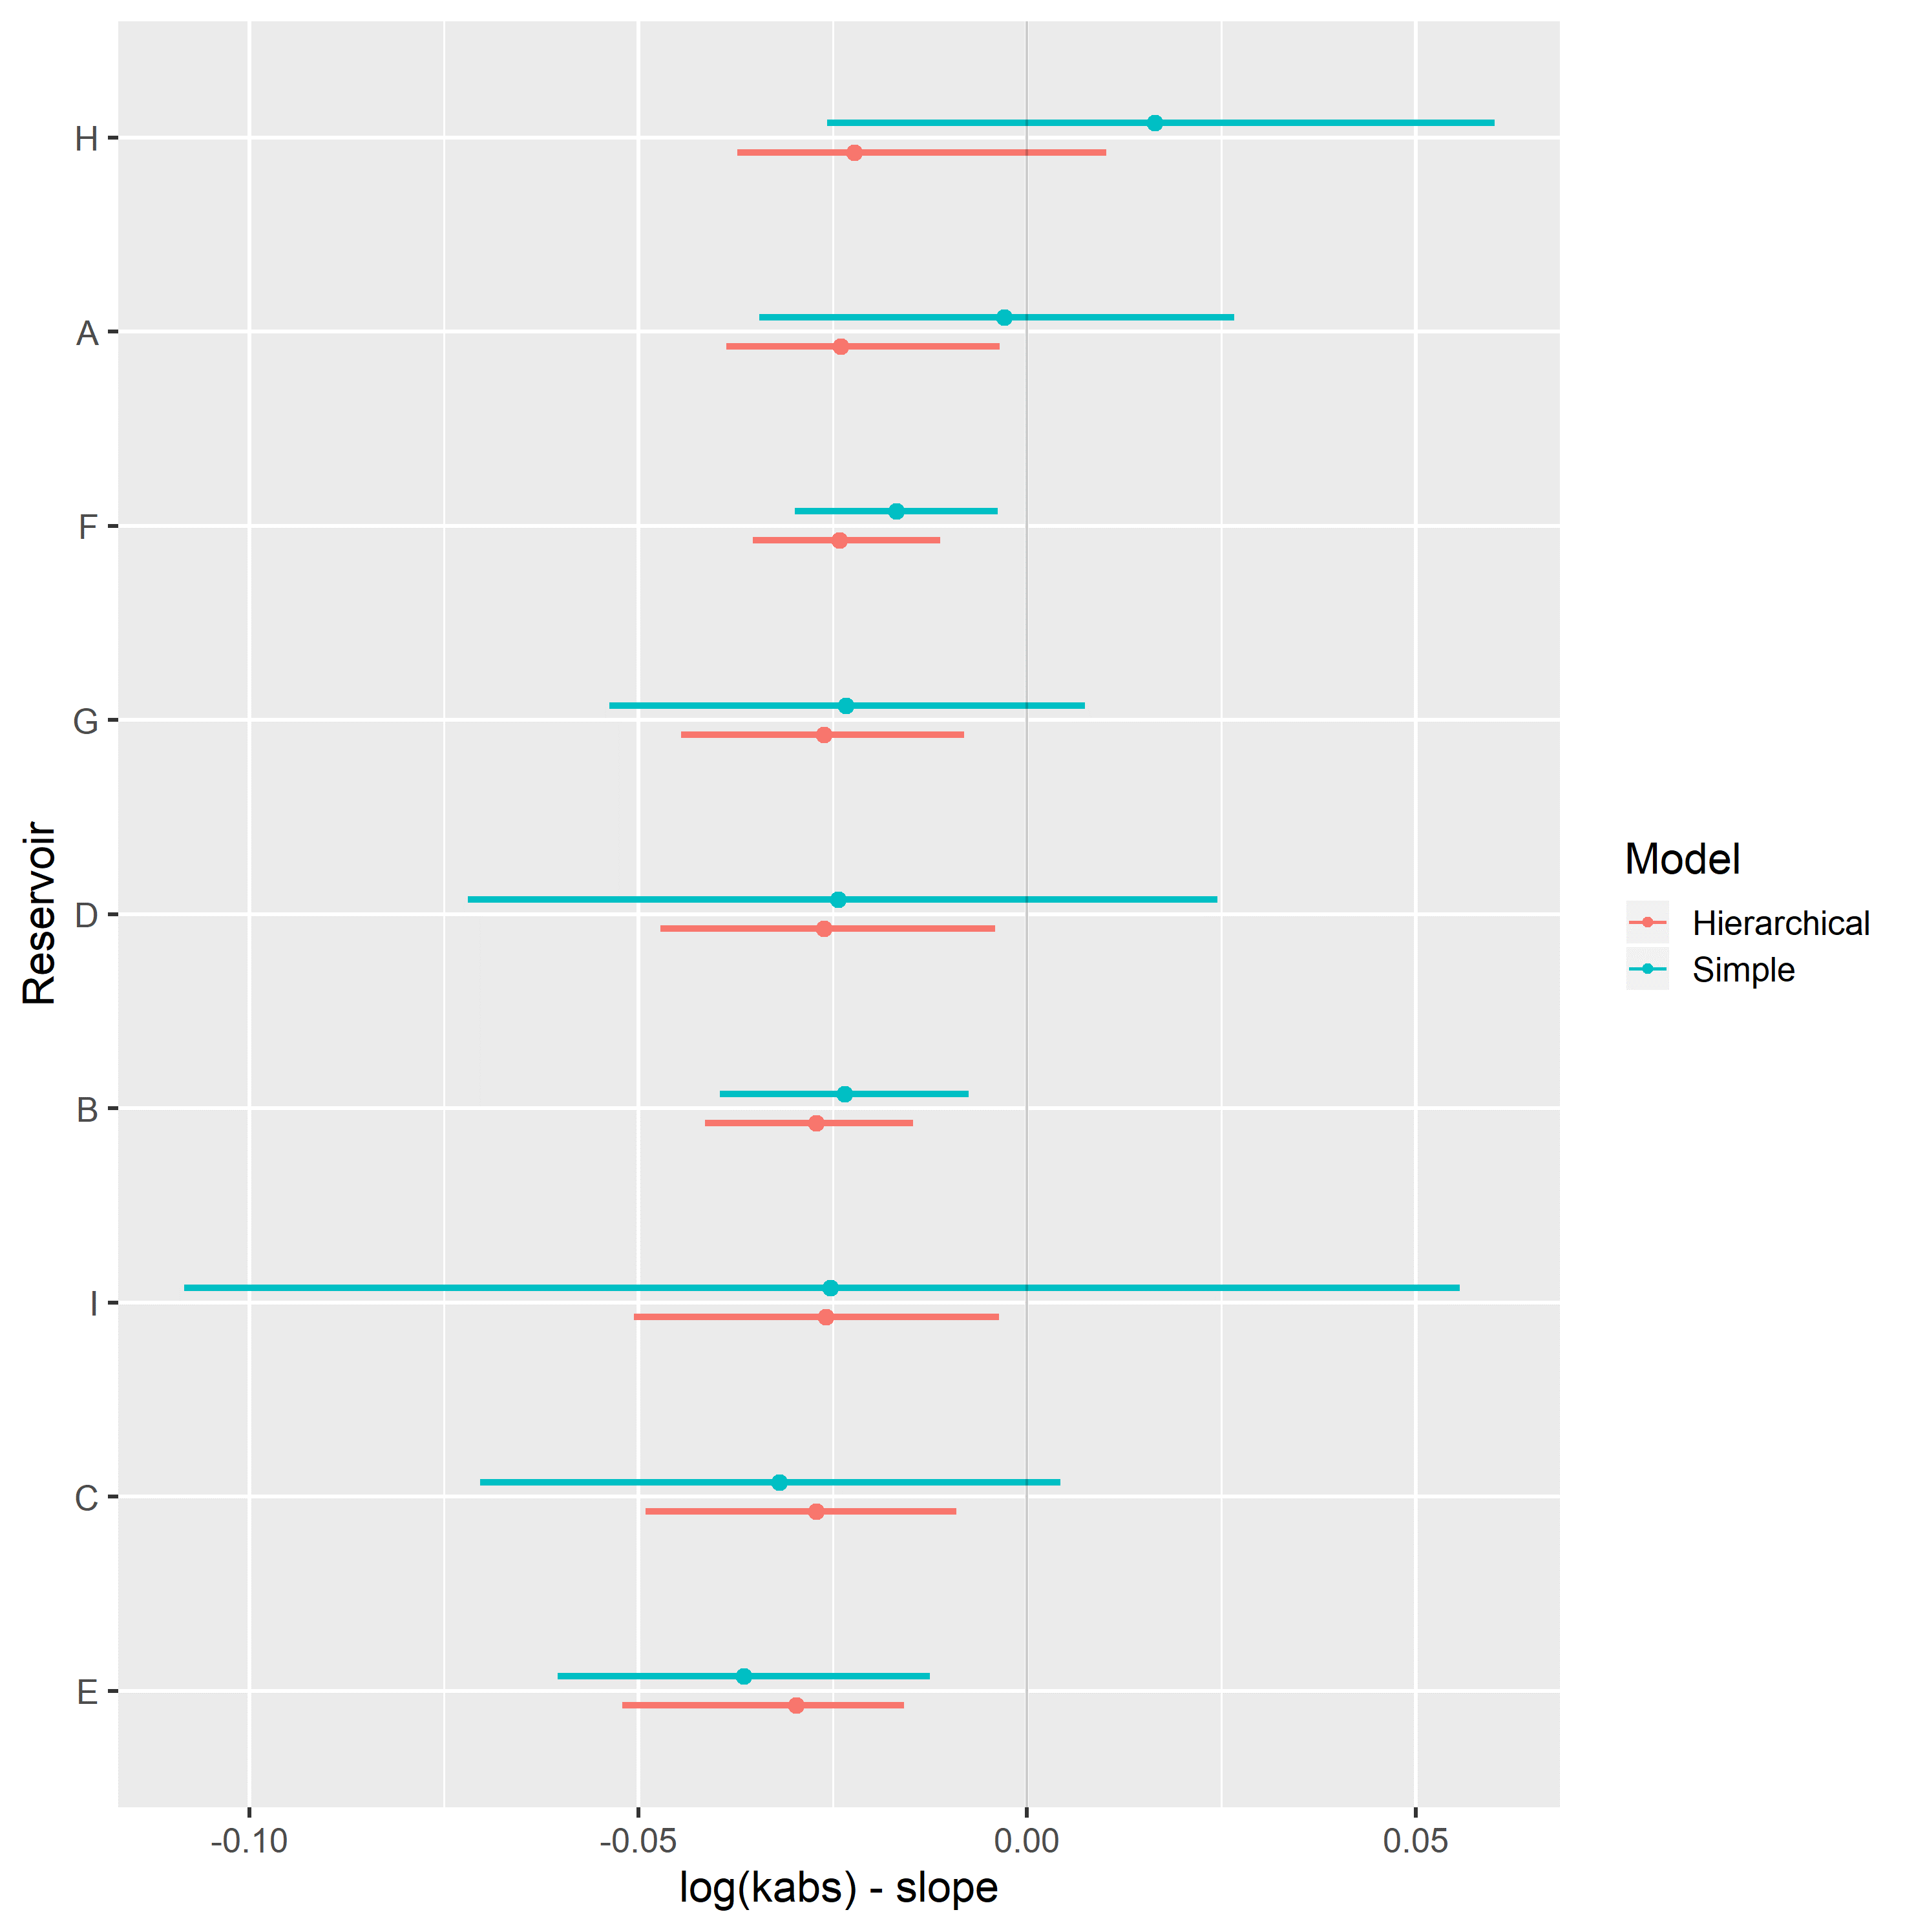
\includegraphics[width=0.75\linewidth]{figure/4-9-swi-coefs-slopes} 
  
  }
  
  \caption{Intercept (top) and slope (bottom), simple and hierarchical linear regression Swi vs log(kabs) model  parameters, grouped by reservoir.}\label{fig:swi-simple-hierarchical-coefs}
  \end{figure}
  \par
  
  Hierarchical varying slope and simple linear regression models of residual oil saturation \(S_{or}\) and logarithm of absolute permeability \(\log{k_{abs}}\) were evaluated on the assembled dataset.
  
  Table \ref{tab:sor-regression-metrics} displays the obtained regression metrics for each fitted model. Both models achieved similar WAIC, LOOIC and \(R_{adj}^2\) metrics.
  \begin{longtable}[]{@{}ccclll@{}}
  \caption{\label{tab:sor-regression-metrics} \(S_{or}\) linear regression model metrics.}\tabularnewline
  \toprule
  \begin{minipage}[b]{0.36\columnwidth}\centering
  Regression Model\strut
  \end{minipage} & \begin{minipage}[b]{0.08\columnwidth}\centering
  RMSE\strut
  \end{minipage} & \begin{minipage}[b]{0.11\columnwidth}\centering
  WAIC\strut
  \end{minipage} & \begin{minipage}[b]{0.09\columnwidth}\raggedright
  LOOIC\strut
  \end{minipage} & \begin{minipage}[b]{0.06\columnwidth}\raggedright
  \(R^2\)\strut
  \end{minipage} & \begin{minipage}[b]{0.13\columnwidth}\raggedright
  \(R_{adj}^2\)\strut
  \end{minipage}\tabularnewline
  \midrule
  \endfirsthead
  \toprule
  \begin{minipage}[b]{0.36\columnwidth}\centering
  Regression Model\strut
  \end{minipage} & \begin{minipage}[b]{0.08\columnwidth}\centering
  RMSE\strut
  \end{minipage} & \begin{minipage}[b]{0.11\columnwidth}\centering
  WAIC\strut
  \end{minipage} & \begin{minipage}[b]{0.09\columnwidth}\raggedright
  LOOIC\strut
  \end{minipage} & \begin{minipage}[b]{0.06\columnwidth}\raggedright
  \(R^2\)\strut
  \end{minipage} & \begin{minipage}[b]{0.13\columnwidth}\raggedright
  \(R_{adj}^2\)\strut
  \end{minipage}\tabularnewline
  \midrule
  \endhead
  \begin{minipage}[t]{0.36\columnwidth}\centering
  Simple Linear Regression\strut
  \end{minipage} & \begin{minipage}[t]{0.08\columnwidth}\centering
  0.09\strut
  \end{minipage} & \begin{minipage}[t]{0.11\columnwidth}\centering
  -414.47\strut
  \end{minipage} & \begin{minipage}[t]{0.09\columnwidth}\raggedright
  -413.64\strut
  \end{minipage} & \begin{minipage}[t]{0.06\columnwidth}\raggedright
  0.18\strut
  \end{minipage} & \begin{minipage}[t]{0.13\columnwidth}\raggedright
  0.11\strut
  \end{minipage}\tabularnewline
  \begin{minipage}[t]{0.36\columnwidth}\centering
  Hierarchical Linear Regression\strut
  \end{minipage} & \begin{minipage}[t]{0.08\columnwidth}\centering
  0.09\strut
  \end{minipage} & \begin{minipage}[t]{0.11\columnwidth}\centering
  -414.40\strut
  \end{minipage} & \begin{minipage}[t]{0.09\columnwidth}\raggedright
  -414.06\strut
  \end{minipage} & \begin{minipage}[t]{0.06\columnwidth}\raggedright
  0.22\strut
  \end{minipage} & \begin{minipage}[t]{0.13\columnwidth}\raggedright
  0.11\strut
  \end{minipage}\tabularnewline
  \bottomrule
  \end{longtable}
  Figure \ref{fig:sor-simple-hierarchical} displays simple and hierarchical linear regression \(S_{or}\) vs \(\log{k_{abs}}\) models, grouped by reservoir. Black dots represent observed samples, light blue lines represent samples from the posterior distribution of intercept and slope parameters, and dark blue lines represent mean intercept and slope parameters, for each reservoir.
  
  Completely pooled, simple linear regression models display larger between-groups slope variations and uncertainty, as shown in Figure \ref{fig:sor-simple-hierarchical-coefs}. Reservoirs with large number of samples, such as reservoir F, show only small changes between hierarchical and simple linear regression model posterior distributions. A stronger regularizing effect is displayed in reservoir I, which contains a small number of samples. Overall behavior consistency of \(S_{or}\) with respect to \(\log{k_{abs}}\) is increased in the hierarchical partially pooled linear model, as slopes are regressed towards a common mean. As information is shared between different reservoirs, posterior uncertainties are noticeably reduced in the hierarchical linear model.
  \begin{figure}
  
  {\centering 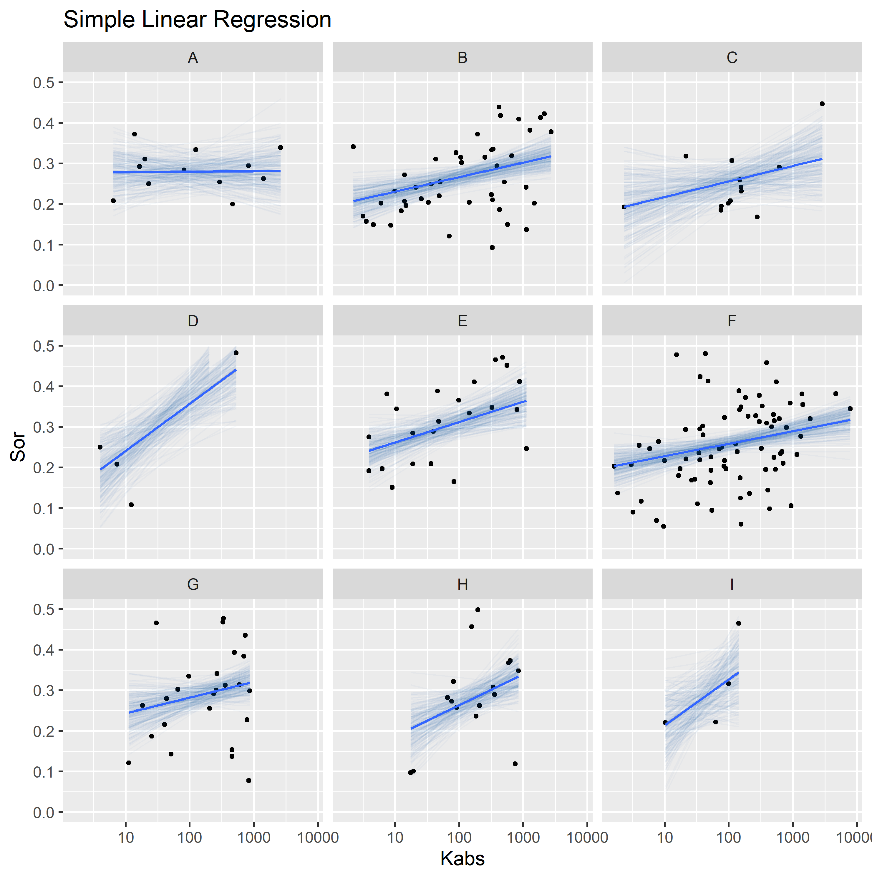
\includegraphics[width=0.75\linewidth]{figure/4-10-sor-simple} \includegraphics[width=0.75\linewidth]{figure/4-10-sor-hierarchical} 
  
  }
  
  \caption{Simple (top) and Hierarchical (bottom) linear regression models of Sor vs log(kabs), grouped by reservoir.}\label{fig:sor-simple-hierarchical}
  \end{figure}
  \begin{figure}
  
  {\centering \includegraphics[width=0.75\linewidth]{figure/4-11-sor-intercept} \includegraphics[width=0.75\linewidth]{figure/4-11-sor-slopes} 
  
  }
  
  \caption{Intercept (top) and slope (bottom), simple and hierarchical linear regression Sor vs log(kabs) model  parameters, grouped by reservoir.}\label{fig:sor-simple-hierarchical-coefs}
  \end{figure}
  \par
  
  Hierarchical varying slope and simple linear regression models of oil relative permeability at irreducible water saturation condition \(k_{ro}@S_{wi}\) and logarithm of absolute permeability \(\log{k_{abs}}\) were evaluated on the assembled dataset.
  
  Table \ref{tab:kro-regression-metrics} displays the obtained regression metrics for each fitted model. Hierarchical linear regression achieved slightly better WAIC, LOOIC and \(R_{adj}^2\) metrics.
  \begin{longtable}[]{@{}ccclll@{}}
  \caption{\label{tab:kro-regression-metrics} \(k_{ro}@S_{wi}\) linear regression model metrics.}\tabularnewline
  \toprule
  \begin{minipage}[b]{0.36\columnwidth}\centering
  Regression Model\strut
  \end{minipage} & \begin{minipage}[b]{0.08\columnwidth}\centering
  RMSE\strut
  \end{minipage} & \begin{minipage}[b]{0.11\columnwidth}\centering
  WAIC\strut
  \end{minipage} & \begin{minipage}[b]{0.09\columnwidth}\raggedright
  LOOIC\strut
  \end{minipage} & \begin{minipage}[b]{0.06\columnwidth}\raggedright
  \(R^2\)\strut
  \end{minipage} & \begin{minipage}[b]{0.13\columnwidth}\raggedright
  \(R_{adj}^2\)\strut
  \end{minipage}\tabularnewline
  \midrule
  \endfirsthead
  \toprule
  \begin{minipage}[b]{0.36\columnwidth}\centering
  Regression Model\strut
  \end{minipage} & \begin{minipage}[b]{0.08\columnwidth}\centering
  RMSE\strut
  \end{minipage} & \begin{minipage}[b]{0.11\columnwidth}\centering
  WAIC\strut
  \end{minipage} & \begin{minipage}[b]{0.09\columnwidth}\raggedright
  LOOIC\strut
  \end{minipage} & \begin{minipage}[b]{0.06\columnwidth}\raggedright
  \(R^2\)\strut
  \end{minipage} & \begin{minipage}[b]{0.13\columnwidth}\raggedright
  \(R_{adj}^2\)\strut
  \end{minipage}\tabularnewline
  \midrule
  \endhead
  \begin{minipage}[t]{0.36\columnwidth}\centering
  Simple Linear Regression\strut
  \end{minipage} & \begin{minipage}[t]{0.08\columnwidth}\centering
  0.20\strut
  \end{minipage} & \begin{minipage}[t]{0.11\columnwidth}\centering
  -48.72\strut
  \end{minipage} & \begin{minipage}[t]{0.09\columnwidth}\raggedright
  -47.50\strut
  \end{minipage} & \begin{minipage}[t]{0.06\columnwidth}\raggedright
  0.34\strut
  \end{minipage} & \begin{minipage}[t]{0.13\columnwidth}\raggedright
  0.28\strut
  \end{minipage}\tabularnewline
  \begin{minipage}[t]{0.36\columnwidth}\centering
  Hierarchical Linear Regression\strut
  \end{minipage} & \begin{minipage}[t]{0.08\columnwidth}\centering
  0.20\strut
  \end{minipage} & \begin{minipage}[t]{0.11\columnwidth}\centering
  -62.02\strut
  \end{minipage} & \begin{minipage}[t]{0.09\columnwidth}\raggedright
  -61.77\strut
  \end{minipage} & \begin{minipage}[t]{0.06\columnwidth}\raggedright
  0.39\strut
  \end{minipage} & \begin{minipage}[t]{0.13\columnwidth}\raggedright
  0.33\strut
  \end{minipage}\tabularnewline
  \bottomrule
  \end{longtable}
  Figure \ref{fig:kro-simple-hierarchical} displays simple and hierarchical linear regression \(k_{ro}@S_{wi}\) vs \(\log{k_{abs}}\) models, grouped by reservoir. Black dots represent observed samples, light blue lines represent samples from the posterior distribution of intercept and slope parameters, and dark blue lines represent mean intercept and slope parameters, for each reservoir.
  
  Completely pooled, simple linear regression models display larger between-groups slope variations and uncertainty, as shown in Figure \ref{fig:kro-simple-hierarchical-coefs}. Reservoirs with large number of samples, such as reservoir F, show only small changes between hierarchical and simple linear regression model posterior distributions. A stronger regularizing effect is displayed in reservoir D, which contains a small number of samples. Overall behavior consistency of \(k_{ro}@S_{wi}\) in respect to \(\log{k_{abs}}\) is increased in the hierarchical partially pooled linear model, as slopes are regressed towards a common mean. As information is shared between different reservoirs, posterior uncertainties are noticeably reduced in the hierarchical linear model.
  \begin{figure}
  
  {\centering \includegraphics[width=0.75\linewidth]{figure/4-12-kro-simple} \includegraphics[width=0.75\linewidth]{figure/4-12-kro-hierarchical} 
  
  }
  
  \caption{Simple (top) and Hierarchical (bottom) linear regression models of kro@Swi vs log(kabs), grouped by reservoir.}\label{fig:kro-simple-hierarchical}
  \end{figure}
  \begin{figure}
  
  {\centering \includegraphics[width=0.75\linewidth]{figure/4-13-kro-intercept} \includegraphics[width=0.75\linewidth]{figure/4-13-kro-slopes} 
  
  }
  
  \caption{Intercept (top) and slope (bottom), simple and hierarchical linear regression kro@Swi vs log(kabs) model  parameters, grouped by reservoir.}\label{fig:kro-simple-hierarchical-coefs}
  \end{figure}
  \par
  
  Hierarchical varying slope and simple linear regression models of water relative permeability at residual oil saturation condition \(k_{rw}@S_{or}\) and logarithm of absolute permeability \(\log{k_{abs}}\) were evaluated on the assembled dataset.
  
  Table \ref{tab:krw-regression-metrics} displays the obtained regression metrics for each fitted model. Hierarchical linear regression achieved slightly better WAIC, LOOIC and \(R_{adj}^2\) metrics.
  \begin{longtable}[]{@{}ccclll@{}}
  \caption{\label{tab:krw-regression-metrics} \(k_{rw}@S_{or}\) linear regression model metrics.}\tabularnewline
  \toprule
  \begin{minipage}[b]{0.36\columnwidth}\centering
  Regression Model\strut
  \end{minipage} & \begin{minipage}[b]{0.08\columnwidth}\centering
  RMSE\strut
  \end{minipage} & \begin{minipage}[b]{0.11\columnwidth}\centering
  WAIC\strut
  \end{minipage} & \begin{minipage}[b]{0.09\columnwidth}\raggedright
  LOOIC\strut
  \end{minipage} & \begin{minipage}[b]{0.06\columnwidth}\raggedright
  \(R^2\)\strut
  \end{minipage} & \begin{minipage}[b]{0.13\columnwidth}\raggedright
  \(R_{adj}^2\)\strut
  \end{minipage}\tabularnewline
  \midrule
  \endfirsthead
  \toprule
  \begin{minipage}[b]{0.36\columnwidth}\centering
  Regression Model\strut
  \end{minipage} & \begin{minipage}[b]{0.08\columnwidth}\centering
  RMSE\strut
  \end{minipage} & \begin{minipage}[b]{0.11\columnwidth}\centering
  WAIC\strut
  \end{minipage} & \begin{minipage}[b]{0.09\columnwidth}\raggedright
  LOOIC\strut
  \end{minipage} & \begin{minipage}[b]{0.06\columnwidth}\raggedright
  \(R^2\)\strut
  \end{minipage} & \begin{minipage}[b]{0.13\columnwidth}\raggedright
  \(R_{adj}^2\)\strut
  \end{minipage}\tabularnewline
  \midrule
  \endhead
  \begin{minipage}[t]{0.36\columnwidth}\centering
  Simple Linear Regression\strut
  \end{minipage} & \begin{minipage}[t]{0.08\columnwidth}\centering
  0.10\strut
  \end{minipage} & \begin{minipage}[t]{0.11\columnwidth}\centering
  -366.62\strut
  \end{minipage} & \begin{minipage}[t]{0.09\columnwidth}\raggedright
  -366.13\strut
  \end{minipage} & \begin{minipage}[t]{0.06\columnwidth}\raggedright
  0.20\strut
  \end{minipage} & \begin{minipage}[t]{0.13\columnwidth}\raggedright
  0.16\strut
  \end{minipage}\tabularnewline
  \begin{minipage}[t]{0.36\columnwidth}\centering
  Hierarchical Linear Regression\strut
  \end{minipage} & \begin{minipage}[t]{0.08\columnwidth}\centering
  0.10\strut
  \end{minipage} & \begin{minipage}[t]{0.11\columnwidth}\centering
  -372.34\strut
  \end{minipage} & \begin{minipage}[t]{0.09\columnwidth}\raggedright
  -372.18\strut
  \end{minipage} & \begin{minipage}[t]{0.06\columnwidth}\raggedright
  0.24\strut
  \end{minipage} & \begin{minipage}[t]{0.13\columnwidth}\raggedright
  0.17\strut
  \end{minipage}\tabularnewline
  \bottomrule
  \end{longtable}
  Figure \ref{fig:krw-simple-hierarchical} displays simple and hierarchical linear regression \(k_{rw}@S_{or}\) vs \(\log{k_{abs}}\) models, grouped by reservoir. Black dots represent observed samples, light blue lines represent samples from the posterior distribution of intercept and slope parameters, and dark blue lines represent mean intercept and slope parameters, for each reservoir.
  
  Completely pooled, simple linear regression models display larger between-groups slope variations and uncertainty, as shown in Figure \ref{fig:krw-simple-hierarchical-coefs}. Reservoirs with large number of samples, such as reservoir F, show only small changes between hierarchical and simple linear regression model posterior distributions. A stronger regularizing effect is displayed in reservoir D, which contains a small number of samples. Overall behavior consistency of \(k_{rw}@S_{or}\) in respect to \(\log{k_{abs}}\) is increased in the hierarchical partially pooled linear model, as slopes are regressed towards a common mean. As information is shared between different reservoirs, posterior uncertainties are noticeably reduced in the hierarchical linear model.
  \begin{figure}
  
  {\centering \includegraphics[width=0.75\linewidth]{figure/4-14-krw-simple} \includegraphics[width=0.75\linewidth]{figure/4-14-krw-hierarchical} 
  
  }
  
  \caption{Simple (top) and Hierarchical (bottom) linear regression models of krw@Sor vs log(kabs), grouped by reservoir.}\label{fig:krw-simple-hierarchical}
  \end{figure}
  \begin{figure}
  
  {\centering \includegraphics[width=0.75\linewidth]{figure/4-15-krw-intercept} \includegraphics[width=0.75\linewidth]{figure/4-15-krw-slopes} 
  
  }
  
  \caption{Intercept (top) and slope (bottom), simple and hierarchical linear regression krw@Sor vs log(kabs) model  parameters, grouped by reservoir.}\label{fig:krw-simple-hierarchical-coefs}
  \end{figure}
  \par
  
  Posterior distribution of latent \(\mu_\alpha\) and \(\mu_\beta\) parameters of hierarchical linear regression models represent average behavior of model parameters across the different evaluated categories. Thus, they represent quantified petrophysical parameter model analogues, and may be used for preliminary characterization of reservoirs with similar characteristics as the ones used in the assembled model, but with no sampled data.
  
  Multi-task simple and varying slopes hierarchical linear regression models, grouped by reservoir, were fitted to the assembled LET relative permeability parameter dataset. Comparison of WAIC and LOOIC metrics between them is shown in Table \ref{tab:multi-task-regression}, displaying slightly better results for the multi-task hierarchical linear regression model.
  \begin{longtable}[]{@{}ccc@{}}
  \caption{\label{tab:multi-task-regression} Multi-task linear regression model metrics.}\tabularnewline
  \toprule
  \begin{minipage}[b]{0.43\columnwidth}\centering
  Regression Model\strut
  \end{minipage} & \begin{minipage}[b]{0.11\columnwidth}\centering
  WAIC\strut
  \end{minipage} & \begin{minipage}[b]{0.13\columnwidth}\centering
  LOOIC\strut
  \end{minipage}\tabularnewline
  \midrule
  \endfirsthead
  \toprule
  \begin{minipage}[b]{0.43\columnwidth}\centering
  Regression Model\strut
  \end{minipage} & \begin{minipage}[b]{0.11\columnwidth}\centering
  WAIC\strut
  \end{minipage} & \begin{minipage}[b]{0.13\columnwidth}\centering
  LOOIC\strut
  \end{minipage}\tabularnewline
  \midrule
  \endhead
  \begin{minipage}[t]{0.43\columnwidth}\centering
  Simple Linear Regression\strut
  \end{minipage} & \begin{minipage}[t]{0.11\columnwidth}\centering
  1119.6\strut
  \end{minipage} & \begin{minipage}[t]{0.13\columnwidth}\centering
  1129.8\strut
  \end{minipage}\tabularnewline
  \begin{minipage}[t]{0.43\columnwidth}\centering
  Hierarchical Linear Regression\strut
  \end{minipage} & \begin{minipage}[t]{0.11\columnwidth}\centering
  1043.3\strut
  \end{minipage} & \begin{minipage}[t]{0.13\columnwidth}\centering
  1048.0\strut
  \end{minipage}\tabularnewline
  \bottomrule
  \end{longtable}
  The posterior distribution of the LET relative permeability parameters for a given reservoir and logarithmic absolute permeability may be used to sample relative permeability curves, fully incorporating the information from the available dataset, as exemplified in Figure \ref{fig:multi-task}.
  \begin{figure}
  
  {\centering \includegraphics[width=0.8\linewidth]{figure/4-16-multi-task} 
  
  }
  
  \caption{Example of multivariate posterior sample of relative permeability curves, fully incorporating the information from the available dataset.}\label{fig:multi-task}
  \end{figure}
  \hypertarget{conclusion}{%
  \chapter*{Conclusion}\label{conclusion}}
  \addcontentsline{toc}{chapter}{Conclusion}
  
  In this work, machine learning and statistical regression models were evaluated for the prediction of routine and special core analysis petrophysical properties on datasets containing experimental results for rock samples from many Brazilian reservoirs.
  
  Several feature engineering and machine learning techniques were evaluated for the estimation of absolute permeability from mercury injection capillary pressure curves. The absolute permeability regression models that achieved the lowest median absolute errors and largest correlation coefficients used the support-vector machine (SVR), random forest or gradient boosted decision trees algorithms, and several features extracted from the mercury porosimetry capillary pressure curve data. Among the linear models for prediction of absolute permeability, the models proposed by Swanson (Swanson \protect\hyperlink{ref-Swanson1981}{1981}) and Winland (Kolodzie \protect\hyperlink{ref-Kolodzie1980}{1980}) obtained the lowest root mean squared errors and highest correlation coefficients.
  
  Using a parametric formulation, special core analysis capillary pressure and relative permeability curve regression problems were framed in a multi-task regression approach. For the estimation of capillary pressure curve parameters, an analytic formulation of the multi-task linear regression problem was considered using the multivariate gaussian conditional distribution. This model was evaluated on an experimental dataset, comparing average predictions and samples from the conditional distribution of parameters, to the observed capillary pressure curve parameters. Although significant dispersion of experimental and predicted parameters values were observed, it was possible to identify that predictions followed expected linear tendencies of capillary pressure curve parameters and absolute permeability.
  
  Posterior distribution of partially pooled varying slopes hierarchical and completely pooled simple linear regression models, with respect to logarithmic absolute permeability, were inferred for relative permeability parameters. Hierarchical linear regression models displayed overall improved information criteria metrics, evaluated using bayesian Watanabe-Akaike and Leave-one-out information criteria. Due to the regularizing effect of the information sharing between different reservoir categories, posterior distribution of relative permeability parameters of hierarchical linear regression models displayed smaller uncertainties and greater consistency.
  
  Posterior distribution of latent parameters of hierarchical linear regression models represent average behavior of model parameters across the different evaluated categories and may be used as quantified petrophysical parameter model analogues for petrophysical characterization of reservoirs with similar characteristics as the ones used in the assembled model, but with no sampled data.
  
  \backmatter
  \bibliographystyle{coppe-unsrt}
  \bibliography{thesis}
  
  \hypertarget{bibliography}{%
  \chapter*{Bibliography}\label{bibliography}}
  \addcontentsline{toc}{chapter}{Bibliography}
  
  \markboth{References}{References}
  
  \setlength{\parindent}{-0.20in}
  \setlength{\leftskip}{0.20in}
  \setlength{\parskip}{8pt}
  
  \hypertarget{refs}{}
  \leavevmode\hypertarget{ref-Albuquerque2018}{}%
  Albuquerque, Marcelo R, Felipe M Eler, Heitor V R Camargo, André Compan, Dario Cruz, and Carlos Pedreira. 2018. ``Estimation of Capillary Pressure Curves from Centrifuge Measurements using Inverse Methods.'' \emph{Rio Oil \& Gas Expo and Conference 2018,}
  
  \leavevmode\hypertarget{ref-AlKhalifah2020}{}%
  Al Khalifah, H., P. W. J. Glover, and P. Lorinczi. 2020. ``Permeability prediction and diagenesis in tight carbonates using machine learning techniques.'' \emph{Marine and Petroleum Geology} 112 (May 2019): 104096. \url{https://doi.org/10.1016/j.marpetgeo.2019.104096}.
  
  \leavevmode\hypertarget{ref-Bentsen1977}{}%
  Bentsen, R G. 1977. ``Using Parameter-Estimation Techniques To Convert Centrifuge Data Into a Capillary-Pressure Curve.'' \emph{Society of Petroleum Engineers Journal} 17 (1): 57--64. \url{https://doi.org/10.2118/5026-PA}.
  
  \leavevmode\hypertarget{ref-Blunt2017}{}%
  Blunt, Martin J. 2017. \emph{Multiphase Flow in Porous Media: A Pore-Scale Perspective}. Cambridge University Press.
  
  \leavevmode\hypertarget{ref-Carpenter2017}{}%
  Carpenter, Bob, Andrew Gelman, Matthew D. Hoffman, Daniel Lee, Ben Goodrich, Michael Betancourt, Marcus A. Brubaker, Jiqiang Guo, Peter Li, and Allen Riddell. 2017. ``Stan: A probabilistic programming language.'' \emph{Journal of Statistical Software} 76 (1). \url{https://doi.org/10.18637/jss.v076.i01}.
  
  \leavevmode\hypertarget{ref-Chen2016}{}%
  Chen, Tianqi, and Carlos Guestrin. 2016. ``XGBoost: A scalable tree boosting system.'' \emph{Proceedings of the ACM SIGKDD International Conference on Knowledge Discovery and Data Mining} 13-17-Augu: 785--94. \url{https://doi.org/10.1145/2939672.2939785}.
  
  \leavevmode\hypertarget{ref-Corey1954}{}%
  Corey, A. T. 1954. ``The Interrelation Between Gas and Oil Relative Permeabilities.'' \emph{Producers Monthly} 38-41.
  
  \leavevmode\hypertarget{ref-Dake2015}{}%
  Dake, L. P. 2015. \emph{Fundamentals fo Reservoir Engineering}. \url{https://doi.org/10.1016/B978-0-08-098206-9.00004-X}.
  
  \leavevmode\hypertarget{ref-DeGroot2012}{}%
  DeGroot, Morris H., and Mark J. Schervish. 2012. \emph{Probability and Statistics}. Edited by Addison-Wesley.
  
  \leavevmode\hypertarget{ref-Forbes1994}{}%
  Forbes, P. 1994. ``Simple and Accurate Methods for Converting Centrifuge Data Into Drainage and Imbibition Capillary Pressure Curves.'' \emph{The Log Analyst}.
  
  \leavevmode\hypertarget{ref-Gelman2014}{}%
  Gelman, Andrew, John B. Carlin, Hal S. Stern, David B. Dunson, Aki Vehtari, and Donald B. Rubin. 2014. \emph{Bayesian Data Analysis}. 3. \url{https://doi.org/10.1017/CBO9781107415324.004}.
  
  \leavevmode\hypertarget{ref-GelmanGoodrich2019}{}%
  Gelman, Andrew, Ben Goodrich, Jonah Gabry, and Aki Vehtari. 2019. ``R-Squared for Bayesian Regression Models.'' \emph{The American Statistician} 73 (3): 307--9.
  
  \leavevmode\hypertarget{ref-Gelman2008}{}%
  Gelman, Andrew, Aleks Jakulin, Maria Grazia Pittau, and Yu Sung Su. 2008. ``A weakly informative default prior distribution for logistic and other regression models.'' \emph{Annals of Applied Statistics} 2 (4): 1360--83. \url{https://doi.org/10.1214/08-AOAS191}.
  
  \leavevmode\hypertarget{ref-Hassler1945}{}%
  Hassler, G. L., and E. Brunner. 1945. ``Measurement of Capillary Pressures in Small Core Samples.'' \emph{Petroleum Transactions of AIME} 160 (1): 114--23. \url{https://doi.org/10.2118/945114-G}.
  
  \leavevmode\hypertarget{ref-Hastie2009}{}%
  Hastie, Trevor, Robert Tibshirani, and Jerome Friedman. 2009. \emph{The Elements of Statistical Learning: Data Mining, Inference, and Prediction}.
  
  \leavevmode\hypertarget{ref-Hoffman2014}{}%
  Hoffman, Matthew D., and Andrew Gelman. 2014. ``The no-U-turn sampler: Adaptively setting path lengths in Hamiltonian Monte Carlo.'' \emph{Journal of Machine Learning Research} 15: 1593--1623. \url{http://arxiv.org/abs/1111.4246}.
  
  \leavevmode\hypertarget{ref-Johnson1959}{}%
  Johnson, E. F., D. P. Bossler, and V. O. Naumann. 1959. ``Calculation of Relative Permeability from Displacement Experiments.'' \emph{Trans. AIME}.
  
  \leavevmode\hypertarget{ref-Kennedy2015}{}%
  Kennedy, Martin. 2015. \emph{Practical Petrophysics}. Vol. 62.
  
  \leavevmode\hypertarget{ref-Kolodzie1980}{}%
  Kolodzie, Stanley. 1980. ``Analysis of Pore Throat Size and Use of the Waxman-Smits Equation to Determine Ooip in Spindle Field, Colorado.'' In \emph{SPE Annual Technical Conference and Exhibition}, 10. Dallas, Texas: Society of Petroleum Engineers. \url{https://doi.org/10.2118/9382-MS}.
  
  \leavevmode\hypertarget{ref-Lenormand2003}{}%
  Lenormand, R. 2003. ``Interpretation of mercury injection curves to derive pore size distribution.'' \emph{International Symposium of the Society of Core Analysts} Internatio: SCA2003--52. \url{https://doi.org/SCA2003-52}.
  
  \leavevmode\hypertarget{ref-Lenormand2016}{}%
  Lenormand, Roland, and Guillaume Lenormand. 2016. ``Recommended Procedure for Determination of Relative Permeabilities.'' \emph{International Symposium of the Society of Core Analysts}, 1--12. \url{https://www.scaweb.org/wp-content/uploads/SCA-2016-Technical-Papers-Tuesday.pdf}.
  
  \leavevmode\hypertarget{ref-Lomeland2005}{}%
  Lomeland, Frode, Einar Ebeltoft, and Wibeke Hammervold Thomas. 2005. ``A new versatile relative permeability correlation.'' \emph{International Symposium of the Society of Core Analysts, Toronto, Canada}, 1--12.
  
  \leavevmode\hypertarget{ref-Mackay2009}{}%
  Mackay, David J. C. 2009. \emph{Sustainable Energy--without the Hot Air}.
  
  \leavevmode\hypertarget{ref-McInnes2018}{}%
  McInnes, L., and J. Healy. 2018. ``UMAP: Uniform Manifold Approximation and Projection for Dimension Reduction.''
  
  \leavevmode\hypertarget{ref-Micromeritics2020}{}%
  Micromeritics. 2020. ``AutoPore IV Series: Automated Mercury Porosimeters.'' \url{https://www.micromeritics.com/product-showcase/autopore-iv.aspx}.
  
  \leavevmode\hypertarget{ref-Migon2015}{}%
  Migon, Helio, Dani Gamerman, and Francisco Louzada. 2015. \emph{Statistical Inference}. Second.
  
  \leavevmode\hypertarget{ref-Nooruddin2013}{}%
  Nooruddin, Hasan A., Fatai Anifowose, and Abdulazeez Abdulraheem. 2013. ``Applying Artificial Intelligence Techniques to Develop Permeability Predictive Models using Mercury Injection Capillary-Pressure Data.'' \emph{SPE Saudi Arabia Section Technical Symposium and Exhibition}, 1--16. \url{https://doi.org/10.2118/168109-MS}.
  
  \leavevmode\hypertarget{ref-Nordtvedt1991}{}%
  Nordtvedt, JE, and K Kolltvelt. 1991. ``Capillary pressure curves from centrifuge data by use of spline functions.'' \emph{SPE Reservoir Engineering}, no. November: 497--501. \url{https://doi.org/10.2118/19019-PA}.
  
  \leavevmode\hypertarget{ref-Peters2012}{}%
  Peters, E. J. 2012. \emph{Advanced Petrophysics}. Austin: Live Oak Book Company.
  
  \leavevmode\hypertarget{ref-Pittman1992}{}%
  Pittman, E. D. 1992. ``Relationship of porosity and permeability to various parameters derived from mercury injection-capillary pressure curves for sandstone.'' \url{https://doi.org/10.1017/CBO9781107415324.004}.
  
  \leavevmode\hypertarget{ref-P.Murphy2012}{}%
  P. Murphy, Kevin. 2012. \emph{Machine Learning: A Probabilistic Perspective}. \url{https://doi.org/10.1007/SpringerReference_35834}.
  
  \leavevmode\hypertarget{ref-Purcell1949}{}%
  Purcell, W. R. 1949. ``Capillary Pressures - Their Measurement Using Mercury and the Calculation of Permeability Therefrom.'' \emph{Journal of Petroleum Technology} 1 (02): 39--48. \url{https://doi.org/10.2118/949039-G}.
  
  \leavevmode\hypertarget{ref-Skuse1992}{}%
  Skuse, Brian, Abbas Flroozabadl, and Henry J Ramey Jr. 1992. ``Computation and Interpretation of Capillary Pressure From a Centrifuge.'' \url{https://doi.org/10.2118/18297-PA}.
  
  \leavevmode\hypertarget{ref-Swanson1981}{}%
  Swanson, B. F. 1981. ``A Simple Correlation Between Permeabilities and Mercury Capillary Pressures.'' \emph{Journal of Petroleum Technology} 33 (12): 2498--2504. \url{https://doi.org/10.2118/8234-PA}.
  
  \leavevmode\hypertarget{ref-Tiab2004}{}%
  Tiab, Djebbar, and E. C. Donaldson. 2004. \emph{Petrophysics: theory and practice of measuring reservoir rock and fluid transport properties}. Boston: Golf Professional Pub.
  
  \leavevmode\hypertarget{ref-Vehtari2017}{}%
  Vehtari, Aki, Andrew Gelman, and Jonah Gabry. 2017. ``Practical Bayesian model evaluation using leave-one-out cross-validation and WAIC.'' \emph{Statistics and Computing} 27 (5): 1413--32. \url{https://doi.org/10.1007/s11222-016-9696-4}.
  
  \leavevmode\hypertarget{ref-Xu2013}{}%
  Xu, C., and C. Torres-Verdín. 2013. ``Pore System Characterization and Petrophysical Classification Using a Bimodal Gaussian Density Function.'' \emph{Math Geosci}.
  
  %\backmatter
  %\bibliographystyle{coppe-unsrt}
  %\bibliography{example}

  %\appendix
  %\chapter{Algumas Demonstra{\c c}\~oes}
\end{document}
